\documentclass[a4paper,12pt]{report}
\usepackage{style}

\begin{document}
\maketitle
\newpage

\begin{center}
    \large Federal University of Mato Grosso do Sul\\
    \large College of Engineering, Architecture and Urbanism and Geography\\
    \large Graduation Programme in Environmental Technologies
    \\[1.5\baselineskip]
    \large\theauthor
    \\[1.5\baselineskip]
    \uppercase{\Large\thetitle}
    \\[1\baselineskip]
\end{center}
\hfill
\begin{minipage}{0.5\textwidth}
A dissertation submitted in partial fulfillment of the requirements for the Master of Science degree in the Graduation Programme in Environmental Technologies in the Federal University of Mato Grosso do Sul, academic area: \textit{Environmental Sanitation and Water Resources}
\\[0.5\baselineskip]
\textbf{Advisors:}\\Prof. PhD. Johannes Gérson Janzen\\
Prof. PhD Carlo Gualtieri (University of Naples Federico II)
\end{minipage}
\\[1\baselineskip]
Approved in: February 22th, 2020
\\[0.5\baselineskip]
\textbf{Dissertation Committee:}
\\[4.5\baselineskip]
\begin{minipage}{0.5\textwidth}
    \begin{center}
    \begin{minipage}{7cm}
        \hrulefill
    \end{minipage}\\
    Prof. PhD. Paulo Tarso de Oliveira Sanches\\
    UFMS
    \end{center}
\end{minipage}
\hfill
\begin{minipage}{0.5\textwidth}
    \begin{center}
    \begin{minipage}{7cm}
        \hrulefill
    \end{minipage}\\
    PhD. Manoel Lucas Machado Xavier\\
    UFMS
    \end{center}
\end{minipage}
\vfill{}
\begin{center}
    \thedate
\end{center}
\pagenumbering{gobble}

The mass within the river...
\chapter*{Resumo}
\pagenumbering{roman}
A hidrodinâmica de zonas mortas foi investigada em dois diferentes tipos de estruturas: cavidades laterais e campos de espigão. Uma revisão de literatura dos principais métodos de investigação deste tipo de escoamento foi conduzida na qual identificamos lacunas a serem preenchidas. A estrutura desta dissertação começa com um modelo numérico de campos de espigão que identificou diferentes fases na qual a troca de massa entre o canal inalterado e a zona morta ocorre. Em seguida, um modelo numérico foi desenvolvido para descrever a hidrodinâmica de uma cavidade lateral usando um método híbrido para calcular os campos turbulentos (\textit{Detached Eddy Simulation}) sob um pacote comercial. Este modelo foi melhorado no seguinte capítulo em uma simulação que considera os campos instantâneos do escoamento (modelo de turbulência \textit{Large Eddy Simulation}) na qual um pacote de código aberto foi utilizado para uma ampliação do acesso do modelo. Finalmente, o principal tópico da dissertação foi descrito e consiste na investigação de uma cavidade lateral vegetada. Neste artigo, descobrimos a presença de uma circulação secundária que não era esperada para essa geometria, caso não houvesse vegetação. Além disso, o artigo trata da análise do escoamento e sua variação em diferentes níveis de densidade de vegetação a qual nos levou a encontrar um valor limite que divide o escoamento.

\chapter*{Dedication}
This is for my beloved Thaís, my parents and JoTa.
I declare that this thesis has been composed solely by myself and that it has not been submitted, in whole or in part, in any previous application for a degree. Except where states otherwise by reference or acknowledgment, the work presented is entirely my own.
\\[3\baselineskip]
  
\hspace{7.5cm}
\begin{minipage}{0.5\textwidth}
    \begin{center}
    \begin{minipage}{8cm}
        \hrulefill
    \end{minipage}\\
    Luiz Eduardo Domingos de Oliveira
    \end{center}
\end{minipage}
\chapter*{Acknowledgements}
I want to thank my family for all of their support. My parents have always provided an example of how to cherish life, to finish difficult tasks, and pushed me to pursue excellence. I want to honour my brother, João, for giving me friendship and an example of living life to the fullest.

I would like to thank Johannes Janzen and Carlo Gualtieri for their direction, drive, and ambition.

I would like to thank Taís N. Yamasaki, Felipe Costa and Filipe Queiroz for boarding the projects and co-authoring many of the here published works.

Also, I would like to thank Taís for helping me to develop this career since my first steps at the laboratory. She has been a great work colleague and a wonderful friend through all these years.

I would like to thank my laboratory colleagues for guiding this journey and for fellowship through out these years. All those coffees were amazing and it was always rewarding and joyful to gather with you.

Thank you to my Lord and Savior Jesus Christ for providing the grace and mercy to sustain and direct me through this endeavour.
This study was financed in part by the Coordenação de Aperfeiçoamento de Pessoal de Nível Superior – Brasil (CAPES) – Finance Code 001

This study was partly conducted in Lobo Carneiro cluster located in NACAD/Coppe - Rio de Janeiro, Brazil

\addcontentsline{toc}{chapter}{Table of contents}
\tableofcontents
\listoffigures
\listoftables

\chapter{Introduction}
\label{chap:introduction}
\pagenumbering{arabic}% Arabic page numbers (and reset to 1)
In this chapter, the topic of this dissertation is first positioned in the research area and its objectives are developed. Following, a more specific definition of the topic will be given. Subsequently, the research objective and hypothesis will be presented.
\section{Background and Motivation}

Accidental pollutant spills in rivers can influence the water quality and the hydrodynamics of the flow over large portions of the channel. Therefore, the calculation of mass transport on rivers is an important aspect to determine the extension of the damage. The parameters that dictate the solute transport in streams and rivers are strongly related to geometric and hydrodynamic characteristics of the river (e.g., velocity distribution, channel width, flow depth, vortex shedding). Over large distances, the mass transport is mainly restricted to the length and thus it takes a 1-dimensional approach \cite{weitbrecht2004}. Although, the complexity of this solute transport must take into account different aspects of the river over its length, as rivers do not have a constant geometry over all its length. The accountability of the cross-section of the river leads to a 2-dimensional model. Despite the model now offer a variability range, there are aspects in natural and regulated rivers that introduce the third dimension due to rapid changes in the depth direction. Still, regions such as dead zones (DZ), that are regions separated from the main channel and have a net flux close to zero in the main stream direction which configures these structures as transient storage volumes. The formation of DZ can occur from any structure that creates an irregularity within the water body morphology, examples of structures are: groyne fields, lateral cavities, vanes, harbours and sidearms. The shared characteristic of these zones is its closeness, except for a single interface, the volume is completely dissociated from the main channel. This implies that the study of this interface is essential to understand all the exchange processes between the DZ and the main channel.

Normally placed in shallow waters, the transport inside the DZ is regarded as a two-dimensional motion, except for the interface between the unaltered channel (main channel) and the DZ where complex three-dimensional motion occurs \cite{xiang2020}. The typical path in the interface follows the order where the fluid penetrates the DZ near the bottom of the channel and exits primarily in the top layer of the flow, also it enters approximately via the downstream portion and exits in the upstream of the DZ \cite{weitbrecht2004,xiang2020}. This structure can be considered as a transient storage volume.

The transient storage of mass inside the DZ has been known to provide refuge to aquatic communities as they seek shelter in slower-moving flows in the surface stream or the hyporheic zone \cite{jackson2013}. According to the same author, the benefits of this storage extends to water quality improvement as the solutes residence times increases further increasing the interaction of nutrient-rich surface waters with biogeochemically-reactive sediments. For instance, \textcite{SchwartzKozerski2003} detected in their sample larger amounts of element contents with sedimentary origin than from geogenic sources, the increase in mass settled to the riverbed. These settled matter can favour vegetation growth (Figure \ref{fig:satelliteImage}). The drag created by the presence of vegetation changes the flow and consequently the mass exchange rates, which increases the uncertainty of volumes captured within the seasons.

\begin{figure}[!ht]
\centering
\begin{subfigure}{0.49\textwidth}
  \centering
  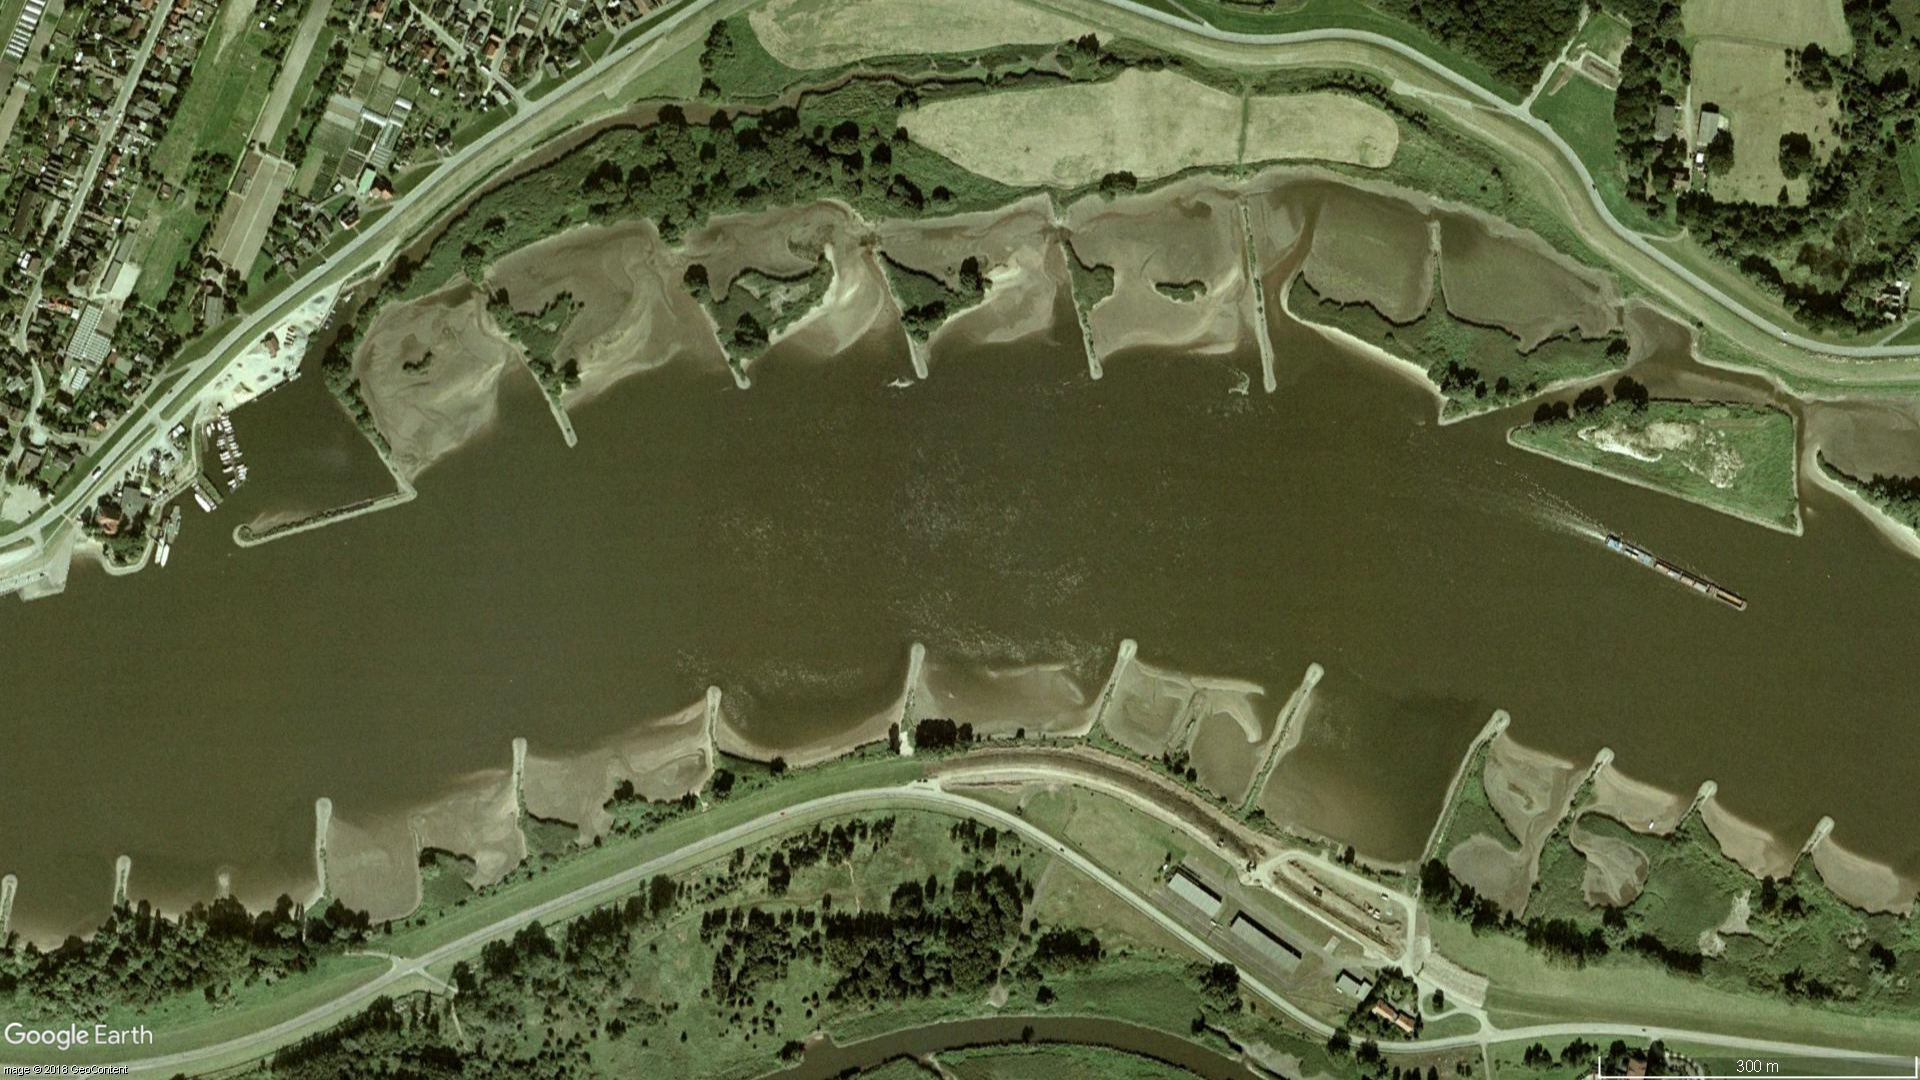
\includegraphics[width=0.9\linewidth]{../images/introduction/sat2000.jpg}
  \caption{2000}
  \label{fig:sat2000}
\end{subfigure}%
\begin{subfigure}{.49\textwidth}
  \centering
  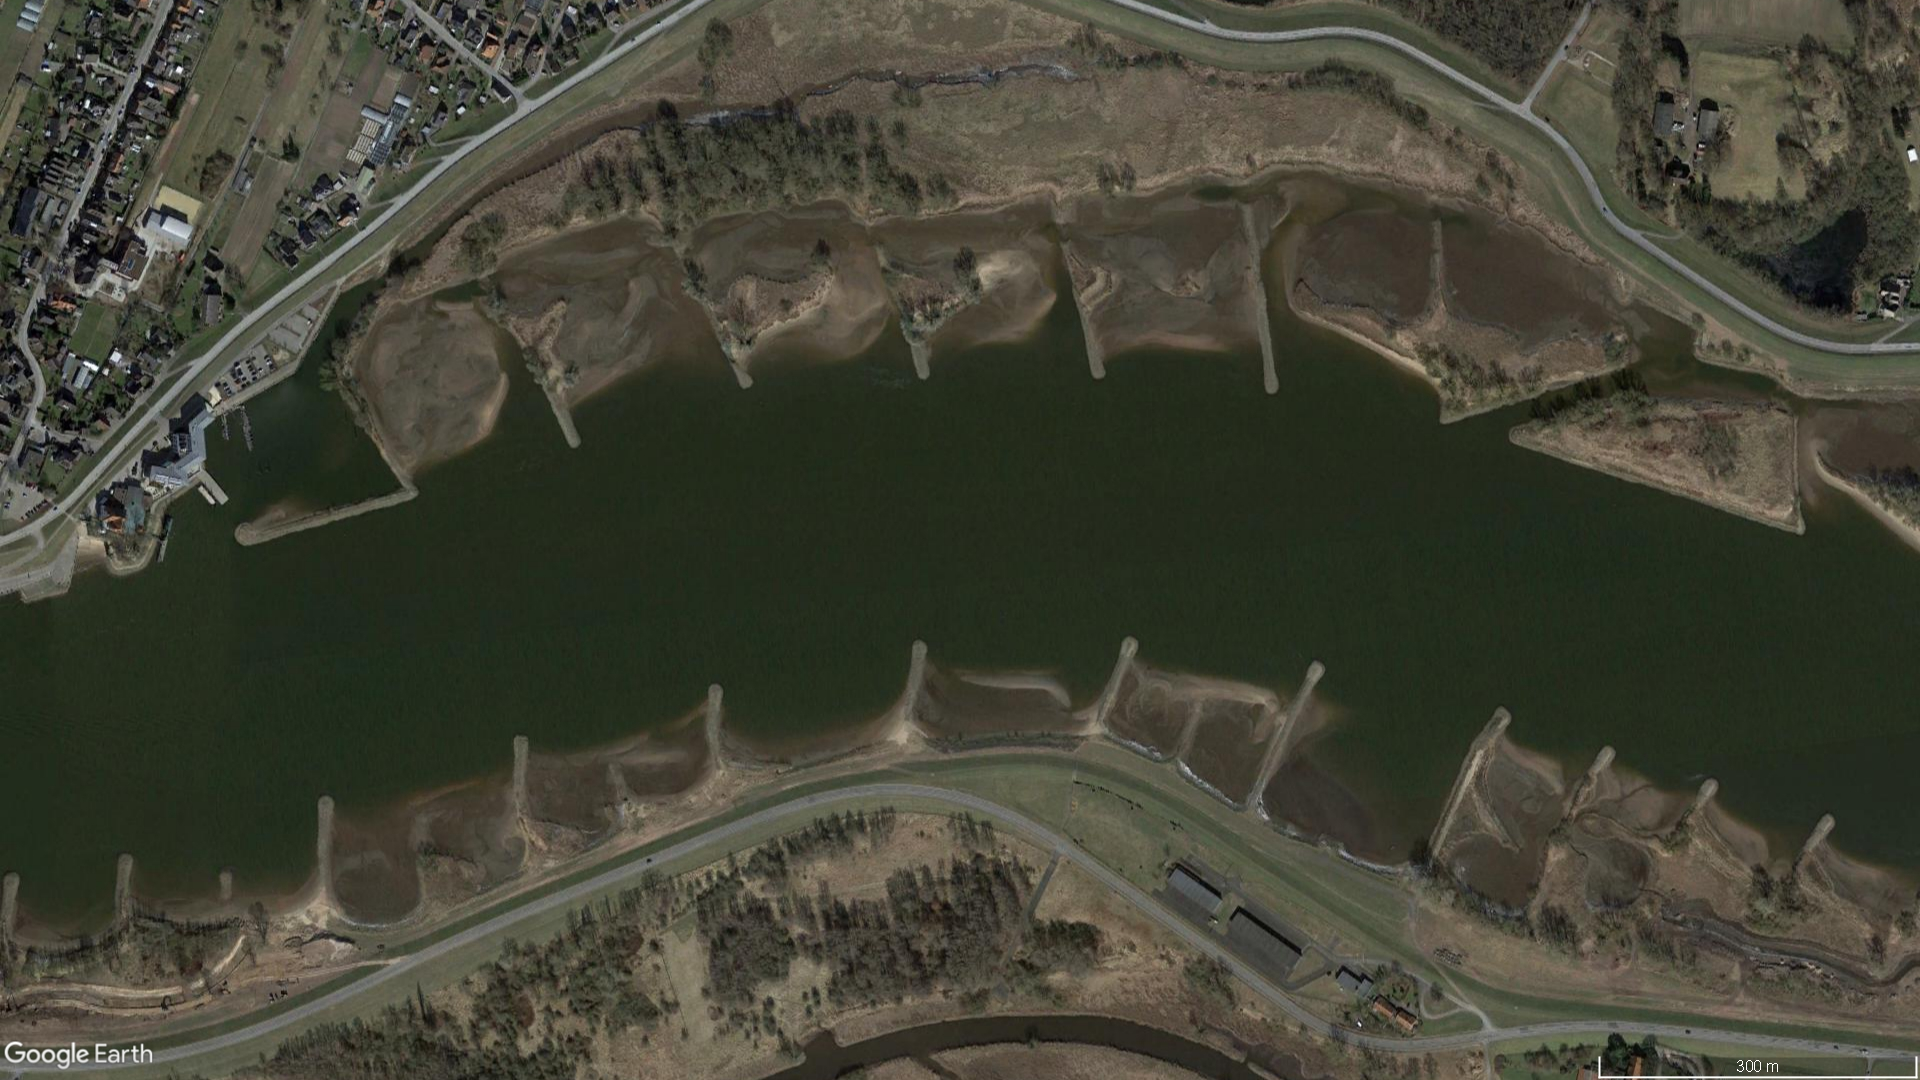
\includegraphics[width=0.9\linewidth]{../images/introduction/sat2018.jpg}
  \caption{2018}
  \label{fig:sat2018}
\end{subfigure}
\caption{Groyne Fields 53\degree23'54.32" N,  10\degree11'51.08" E, elevation 1.90 km. Terrain layer, viewed 29 August 2019. <http://www.google.com/earth/index.html>}
\label{fig:satelliteImage}
\end{figure}
\section{Hydrodynamics and Mass Exchange}
The DZ is created by transversal structures placed on the riverbank, these structures diverge the flow creating a rotational field. The importance of DZ is due (1) the enhancement in biodiversity \cite{ribi2014,harvey2016}, (2) the function as a macro-roughness at the river banks, mitigating erosion \cite{Juez2018} and (3) act as a transient storage zone \cite{jackson2013,drost2014,jackson2015}. The principal characteristic of the flow, in an emergent scenario, is the presence of gyres. These vortexes origin from the dissipation of moment that occurs in the interface layer between the DZ and the main channel. The shearing and flow separation at the leading edge form a mixing layer that extends until the downstream portion of the lateral cavity \cite{uijttewaal2005,jackson2013}. The shape and quantity of circulations inside the cavity are determined by a geometric aspect between the width (normal to the flow, \textit{W}) and length (parallel to the flow, \textit{L}) of the cavity. The aspect ratio \textit{W/L} divides the flow in three configurations: (a) $W/L<0.5$ results in multiple circulations parallel to the main stream; (b) $0.5<W/L<1.5$ results in a single circulation; and (c) $W/L>1.5$ results in multiple gyres transversal to the main stream \cite{weitbrecht2001,jackson2013,sukhodolov2014}(Figure \ref{fig:lCavitySchema}).

The number of circulations in the system impacts on the mass exchange between the DZ and the main channel. As the mass decay inside the DZ follows a quick exponential decay in the early stages the rates get slower as the primary gyre transfers its mass out, in multiple gyres systems \cite{jackson2012,deOliveira2020}. After the main gyre transfers its mass, a slower exchange takes place between the second circulation into the primary one, since the velocity magnitudes in the secondary gyre are slower than the primary one. Henceforth, the mean residence time inside the DZ depends on the primary gyre residence time (early decay) and the secondary gyre volume (late decay) \cite{jackson2013,deOliveira2020}.

From all the different structures that can create a DZ this study will focus on lateral cavities and groynes. A lateral cavity is a volume, normally, adjacent to the riverbank as an external structure (Figure \ref{fig:lCavitySchema}). Groynes consist of a series of lateral cavities, normally, inside the channel course (Figure \ref{fig:satelliteImage}). The characteristics of the flow in both structures are similar. Although an important difference is in the stabilisation of the mixing layer, this region grows until the fourth-sixth rank until it reaches a developed state for groynes (Figure \ref{fig:groyneStabilisation}), in other words, once it stabilises the width of the interface the flow becomes \textit{permanent} \cite{weitbrecht2004, mcCoy2008, xiang2020}. This behaviour is a key aspect for modellers as this is a way to save computational resources and still maintain the comprehensiveness of the model.

\begin{figure}[!ht]
\centering
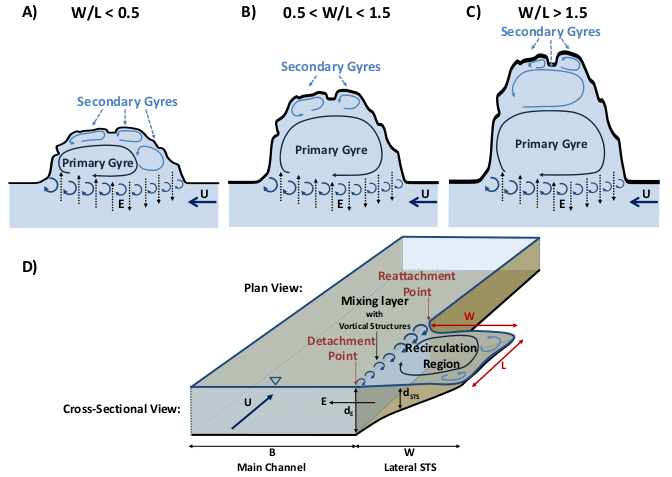
\includegraphics[width=0.9\linewidth]{../images/introduction/lateralCavitySchema.png}
\caption{Schema on the flow patterns of emergent lateral cavities \cite{jackson2013}}
\label{fig:lCavitySchema}
\end{figure}

\begin{figure}[!ht]
\centering
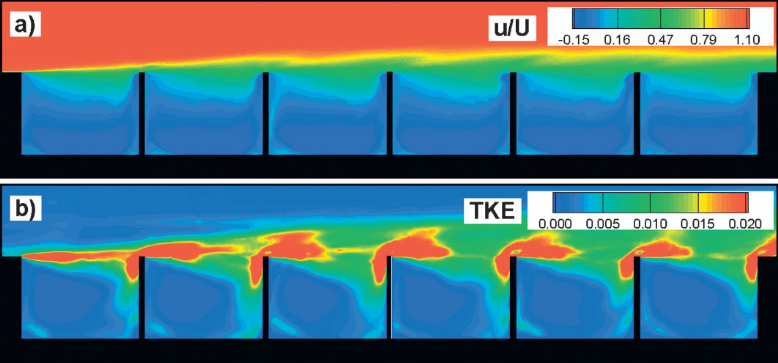
\includegraphics[width=0.9\linewidth]{../images/introduction/groyneStabilisation.png}
\caption{Time averaged quantities at $z/h=0.95$: a) streamwise velocity and b) TKE \cite{mcCoy2008}}
\label{fig:groyneStabilisation}
\end{figure}

The mass exchange between DZs and the main channel was vastly studied in field, experimental and numerical studies. Two different methods to estimate the velocity in which this exchange occurs are predominant: interface velocity measurements and tracer experiments.

As the effects of the exchange occur in a confined volume, \textcite{weitbrecht2001} proposed a model to account the exchanges in the interface between the zones. This method only requires geometrical parameters and the mean transversal velocity in the interface surface. Despite this planar method give a good approximation on the exchange velocity the effect of mass diffusivity and depth variation is neglected,  this further implies that systems slower circulations will have a larger impact of the estimated $k$, as the interface between the main channel and the cavity may remain with faster velocities. One can assume that this methodology works for conventional DZ, although it must be taken carefully for vegetated systems as the mixing layer alone may influence the result of $k$. 

Another approach on the mass exchange is through tracer experiments, that can be divided into washout and pulse procedures, that consists in the ejection of mass from the interior of the DZ and a pulse at the inlet of the channel, respectively.  Tracer methods treat the mass exchange tri-dimensionally as all the flow variables are considered. This approach gives a better understanding of the exchange in all conditions as it provides more information, for instance, the tracer methodology allows one to study the behaviour of mass in local regions of the volume or as a global volume. Furthermore, the coherent structures of the interface play a significant role in the transport of the tracer, given that the turbulence motion is transient, this method can capture the mass exchange rates over time and provide a better insight of the effect of those flow structures.

The advantage of the tracer method is the data richness that it provides, especially in numerical experiments. Some additional studies can be done to analyse other phenomena associated to mass, for instance, one can use a decay to estimate the amount of mass that is treated by plants or a settling velocity to preview sedimentation in the DZ. The only side effect of this method is the increased complexity to perform these experiments, be the difficulty in controlling the volume of water in the field or the calibration of the turbulent Schmidt number ($S_{ct}$) in numerical studies. 
\section{Ecology and Vegetation}
The presence of vegetation in river can also influence the hydrodynamics of the DZ and ,thus, the dispersion of solutes. Since the vegetation cover in rivers is dynamic, changing with seasonality and global climatic change, the dispersion of solutes in rivers is also dynamic. \cite{sukhodolova2006}, for example, studied the influence of the seasonality upon the longitudinal dispersion in a lowland river with vegetation. They observed that when vegetation is absent, the dead zones are represented predominantly by recirculation zones formed by flow separation on bank irregularities; in vegetative period, the dead zones are formed by blocking effect of vegetation occupying part of the river cross-section. These dead zones cause an increase of longitudinal dispersion, which means stronger lengthening of a solute cloud in the mainstream direction \cite{weitbrecht2004}.

The influence of vegetation in the mass exchange in lateral cavities was first studied in \textcite{xiang2019}, that will be discussed in this paragraph. In this paper, a single lateral cavity was studied with a varied vegetation density. The vegetation was represented as solid cylinders inside the cavity volume. The cavity was emergent with a single circulation, due to its $W/L=0.6$. The vegetation density ($a$) ranged from 0 to $6.27\permil$ and as it increased more drag was introduced into the flow resulting in a slower circulation inside the volume. The turbulent kinetic energy in the DZ gradually due to the blockage that impeded high energy vortexes from entering the volume. The effect on mass exchange occurred in two phases: first, there was a decay in the mean residence time due to the plant induced Karman vortex street and the plant blockage since the mixing rate from the vortex is greater than the blockage; in a second phase $a>3.96\permil$ the blockage was higher than the mixing what increases of mean residence time (Figure \ref{fig:xiang2019fig12}).
\begin{figure}[!ht]
\centering
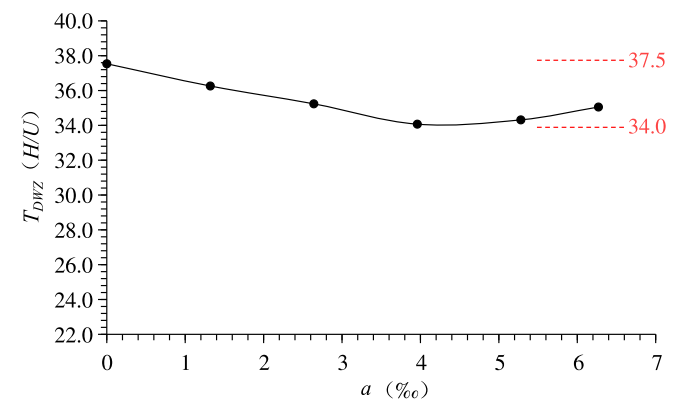
\includegraphics[width=0.8\linewidth]{../images/introduction/xiang2019fig12.png}
\caption{The variation of mean residence time ($T_{DWZ}$) with the increase of vegetation density ($a$) \cite{xiang2019}.}
\label{fig:xiang2019fig12}
\end{figure}

Although researchers have been studying the effect of groynes and vegetation on dispersion of solutes in rivers over the last decades (e.g. \textcite{sukhodolov2017,xiang2019,xiang2020}, there are still issues to that were not examined. For instance, in a vegetated groyne the vegetation levels were up to $15.7\permil$ \cite{sukhodolov2017}, a larger vegetation density range may contain other phenomena that could not appear in the previous studies. This hypothesis indicates that studying the variation of density until the vegetation resistance blocks the flow would cover all the possible ranges and thereby phenomena associated with this flow. Second, up to now the effects of the vegetation on the instantaneous fields were not investigated on lateral cavities. Third, the mass transfer at the main channel/dead zone was mainly studied using only the velocity at the interface, this leads to the opportunity of further describe the behaviour of mass inside the dead zone volume and how it affects the total exchange.

Furthermore, the study with vegetated cavities still could not identify a threshold for vegetation to be considered "dense" or "sparse" in cavities, and its understanding will allow researchers to identify flow modifications in the cavity (e.g., the suppression of recirculation gyres, the complete suppression of flow, the exchange coefficient asymptote, etc.).  For emergent vegetation patches in an open channel, \textcite{chen2012} characterised them as being “dense” or “sparse” according to flow blockage thresholds, in which the flow properties near the patch (e.g., flow adjustment length and the velocity exiting the patch) were distinct above and below the threshold. A similar approach can be done for vegetated cavities. 
\section{Objective and Research Questions}
In order to address this issues, the objective of this study is:

\textit{To describe the hydrodynamics and the mass exchange between vegetated dead waters and
the undisturbed section of the flow for different vegetation densities.}

The main hypothesis is that there is a threshold between dense and sparse vegetation in dead water. We also hypothesised that there is a threshold where the flow ceases inside the lateral cavity. 

Specific methodological objectives:
\begin{itemize}[noitemsep,topsep=0pt,align=left,itemindent=\parindent]
    \item The choice of the modelling technique;
    \item The choice of the modelling package (open and commercial software);
    \item The method to represent the vegetation drag.
\end{itemize}

\section{Dissertation Structure}
The dissertation was divided into six chapters. Following the Introduction, the first paper is presented where the methodology of the study of groyne fields is firstly introduced. Thirdly, the presented paper discussed the first approach to the study of lateral cavities. Fourthly, further development of the numerical model is presented, this implementation focused on the accessibility of the model by making use of open-source tools. Fifth, the main topic of this dissertation is introduced in the paper that describes the influence of the vegetation density in lateral cavities. Finally, the conclusive remarks about the flow in DZ and its mass exchange were presented.


\chapter{Mass Exchange in Dead Water Zones: A Numerical Approach}
\label{chap:art1}
In this chapter, the first topic of the dissertation is presented as a published conference paper. The objective of this paper was to develop a simple numerical method capable of estimating the flow and the mass exchange between consecutive groyne fields and the main channel.

The original paper was published in the book 'Water, Energy and Food Nexus in the Context of Strategies for Climate Change Mitigation', under Spring publishing and can be found in \url{https://www.springer.com/gp/book/9783030572341}.
\section*{Authors}
\begin{itemize}
    \item Luiz Eduardo Domingos de Oliveira \footnote[1]{Federal University of Mato Grosso do Sul}
    \item Johannes Gérson Janzen \footnotemark[1]
\end{itemize}
\addcontentsline{toc}{section}{Abstract}
\section*{Abstract}
Dead water zones (DWZs) in natural open channels, formed by consecutive groynes, are regions separated from the main channel, characterized by recirculating flows. These regions present smaller velocities compared to the main channel, increasing the deposition of sediment and the temporary storage of polluted materials. Exchange processes between DWZs and the main channel influence the transport of pollutants in channels. This study adopts the k-omega shear stress transport (SST) turbulence model to examine the mass exchange between the main channel and the DWZ created by an infinite series of groynes. The computational results were compared to data collected in literature. A good agreement was achieved in mass exchange coefficient, with a relative error of approximately 2\%.

\noindent\textbf{Keywords:} Dead water zones (DWZ); Groyne Fields; Mass Exchange; Open Channel; Computational Fluid Dynamics (CFD).

\section{Introduction}
In fluvial engineering, channels are generally shaped by complicated boundaries that can be composed by dead water zones (DWZ), which can be formed by consecutive groynes \cite{xiang2019}. Groynes are transversal dykes placed in sequence along riverbanks keeping the flow away from the banks. The effects of this structure in rivers are an increase in mean velocity and water depth in the main channel, improved navigability; increased efficiency of sediment transport; protection against flooding and the mitigation of bank erosion \cite{mcCoy2008}. Its placement also provides lateral heterogeneity that can favour the presence of aquatic organisms, improving the biodiversity of river ecosystems \cite{mcCoy2008,Szlauer-ukaszewska2015,Buczynski2017,Mignot2017,Buczynska2018,xiang2019}.

Since the magnitude of mean flow velocities inside the DWZ is approximately 25\% of the flow velocities in the main channel, not only the deposition of sediment is enhanced, but also nutrients and contaminants which are readily attached to fine particles \cite{sukhodolov2014}. For instance, the attachment of contaminants to particles was observed in the Middle Elbe River, in Germany, leading to a low standard classification from an ecological view \cite{SchwartzKozerski2003}. The authors found, in the groyne fields, the deposition of fresh organic mud with high nutrient and pollution content (e.g. nitrogen). The deposition of pollution content attached to sediments creates a problem for river management \cite{uijttewaal2005}, especially in flood seasons, when the groyne field becomes submersed, being a source of contaminants to the main channel.

Therefore, in order to estimate the transport of pollutants in a channel, it is important to be able to understand and predict the exchange processes between the main channel and the DWZ formed between groynes \cite{weitbrecht2001}. These exchange processes were studied in detail in a series of laboratorial experiments carried out by \textcite{weitbrecht2004}. \textcite{Hinterberger2007} used large eddy simulation (LES) to model Weitbrecht’ experimental results. Although being a very precise model, LES is also more time consuming when compared to simpler models. Therefore, this study aims to investigate the mass exchange between the main channel and the groyne field using a simpler two-equations turbulence model, k-omega SST. The computational results are compared to Weibrecht results and a good agreement was obtained.

\section{Methods}
The geometry was chosen to match the groynes from the second series of experiments described in \textcite{weitbrecht2004}. The flow depth ($h$) was kept constant at 0.046 m and the experimental channel width ($B$) at 1.80m. The emergent groynes were 0.50m long ($W$) and spaced 1.25m apart ($L$), producing an aspect ratio of $W/L = 0.40$. The groyne heads were in a semi-circle format with diameter of 0.05m. The Reynolds number was 7360, and thereby turbulent.

The flow past the most downstream-located groyne in the series had a periodic behaviour \cite{Hinterberger2007}. Consequently, only one complete groyne field and two halves (located upstream and downstream from the complete one) was computed and a translational periodic boundary condition was imposed (Figure \ref{fig:art1:numericalDomainArticle1}). The mean streamwise velocity in the computational domain was approximately $U = 11 cm/s$, which corresponds to a mass flux of 6.56 kg/m² of water in the periodic zones. 

As the effects of the obstacles in the main channel extends up to one obstacle length in the transversal direction (y-axis) \cite{Brevis2014} the domain was two-thirds of the experimental flume width (B), reducing the computational effort. A free-slip symmetry boundary condition was imposed on the surface (Figure \ref{fig:art1:numericalDomainArticle1}). This boundary condition was also used on the free surface plane as it is an acceptable simplification for flows with Froude numbers smaller than 0.5 (our Froude number was 0.24) \cite{alfrink1983}. All walls, bed, lower side wall and groyne walls were considered hydraulically smooth.

\begin{figure}[!ht]
\centering
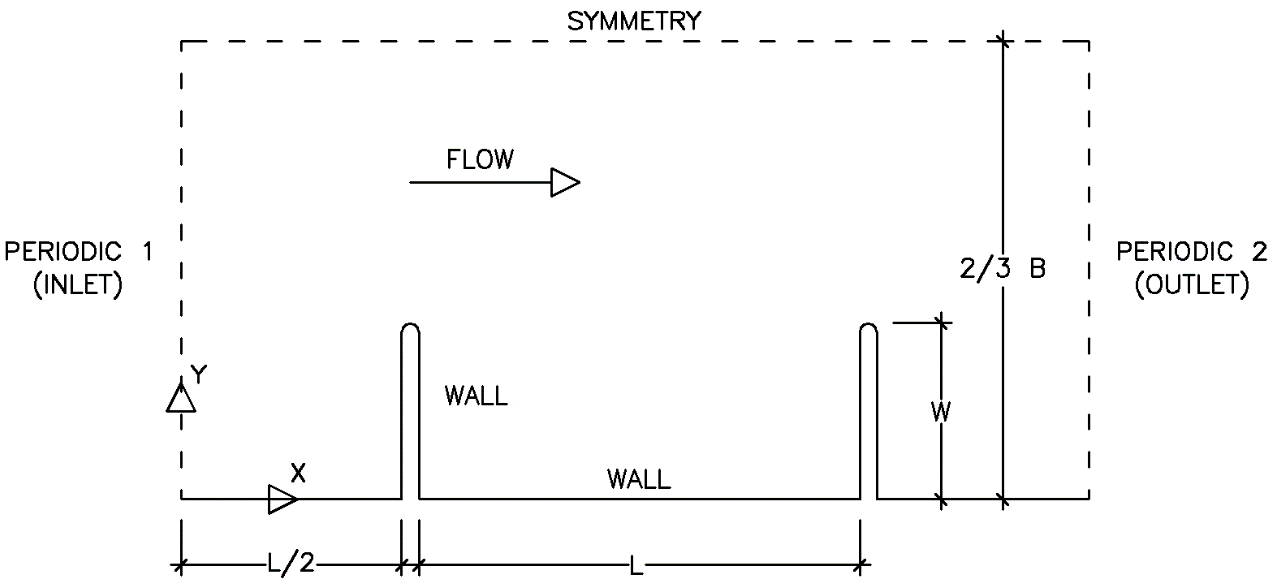
\includegraphics[width=\linewidth]{../images/art1/imgMassExchange1.png}
\caption{Upper view of the computational domain, from the free surface, and its boundary conditions.}
\label{fig:art1:numericalDomainArticle1}
\end{figure}

The domain was calculated in a three-dimensional grid (Figure \ref{fig:art1:mesh} a). The spatial discretization had a higher refinement in regions close to walls and at high velocity gradients regions. The meshing of the groyne’s heads considered its curvature and the proximity to the wall. This region used an O-grid with increasing element size (Figure \ref{fig:art1:mesh} b). The mesh had 20 divisions in the z-axis, increasing gradually from the bottom of the channel to its free surface (Figure \ref{fig:art1:mesh} c). In the y-axis, the groyne field had 70 divisions that gradually increased in size as it gets closer to the middle of the field. The strip that contains the groyne’s heads had finer elements due to the momentum transfer in the shear layer. The total grid presented approximately one million elements.

The commercial software called Ansys® FLUENT (version 14) was used to solve the grid, using the finite volume method to discretize the governing mass and momentum equations. The turbulent model chosen is based at Reynolds-averaged Navier-Stokes equations (RANS) approach, that consists of time averaged equations for fluid flow. The turbulent calculations were solved using the k-omega SST model proposed by \textcite{Menter2005}, due to its capability of solving fluid flow in low Reynolds numbers. The pressure-velocity coupling method was SIMPLE and the gradient spatial discretization was Least Squares Cell Based. The momentum was discretized in a third order MUSCL scheme. The turbulent kinect energy ($tke$) and specific dissipation rate ($\omega$) were discretized in a second order upwind scheme.

In addition to the velocity field, tracer concentration fields were also calculated by solving the following transport equation 
\begin{equation}
\frac{\partial}{\partial t}(\rho Y_i)+\nabla (\rho \vec{v} Y_i)=\nabla (\rho D_{i,m}+\frac{\mu_t}{Sc_t})\nabla Y_i
\label{eqn:art1:transportEq}
\end{equation}\begin{equation}
Sc_t = \frac{\mu_t}{\rho D_t}
\label{eqn:art1:Sct}
\end{equation}
where $\rho$ is the fluid mass density, $Y_i$ is the local mass fraction of each species, $D_{i,m}$ is the mass diffusion coefficient for species in the mixture, $\vec{v}$ is the velocity vector, $Sc_t$ is the turbulent Schmidt number (Equation \ref{eqn:art1:Sct}), $\mu_t$ turbulent viscosity and $D_t$ the turbulent diffusivity. In other terms, the transport equation means that the rate of change and the net rate of flow (convection) equals the rate of change due to diffusion.

Equation (\ref{eqn:art1:transportEq}) does not consider any chemical reactions or addition of phases during the solution and was discretized in a second order upwind scheme. The tracer was conservative, pursuing the same properties than water.

\begin{figure}[!ht]
\centering
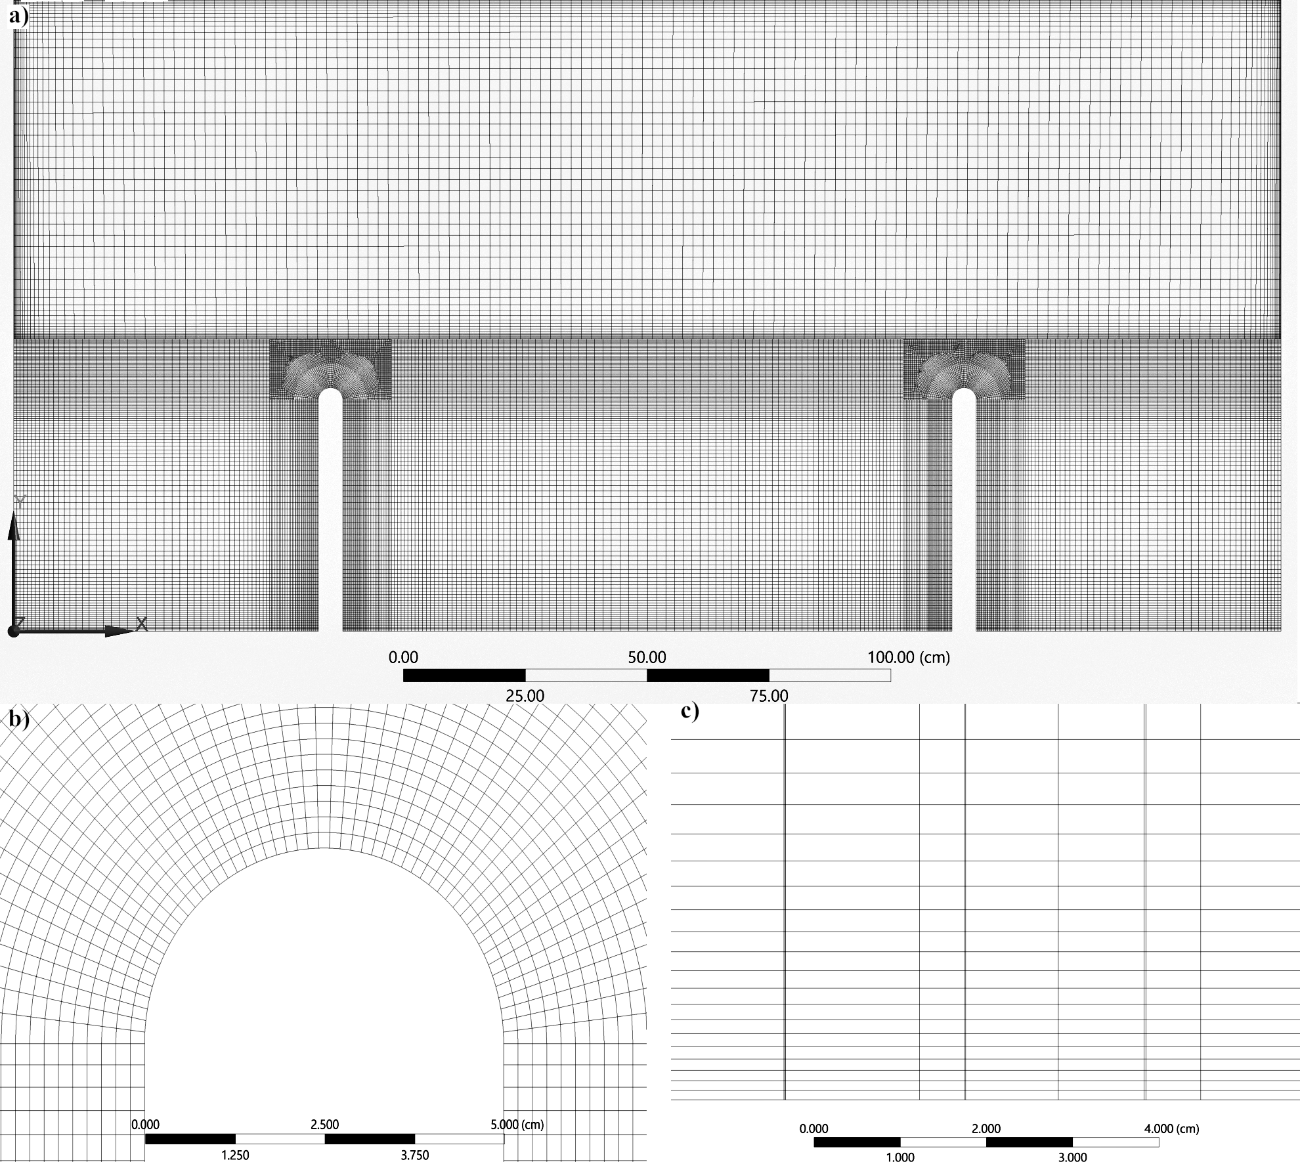
\includegraphics[width=\linewidth]{../images/art1/imgMassExchange2.png}
\caption{Computational mesh: a) mesh in the free-surface plane; b) curvilinear grid around groyne tip; c) mesh in a vertical plane near the middle of the groyne field.}
\label{fig:art1:mesh}
\end{figure}

The time step in the simulation was $0.024h/U$. The simulation was run for nearly $180h/U$ until the fully developed state was achieved. Once the flow reached the fully developed state, the tracer mass fraction was set to 1 within the groyne field and 0 in the other parts of the channel. Then, statistics of the mean flow and tracer transport were calculated using the instantaneous flow fields and mean tracer concentration inside the groyne field over the next $548h/U$.

\section{Results and Discussion}
Two gyres could be observed in the groyne field. A large primary gyre (right vortex in the central groyne field) and a small secondary gyre in the upstream groyne (Figure \ref{fig:art1:contour}). The formation of this system occurred by the momentum transferred by the main channel through a mixing layer. As the main flow went downstream, the shear in between zones excited an anticlockwise gyre (primary gyre) that further excited a smaller clockwise circulation (secondary gyre) that had no contact with the main channel. The secondary gyre was smaller in size (approximately 21\% of the groyne field area) and velocity magnitudes, when compared to the mean circulation (Figure \ref{fig:art1:contour}).

\begin{figure}[!ht]
\centering
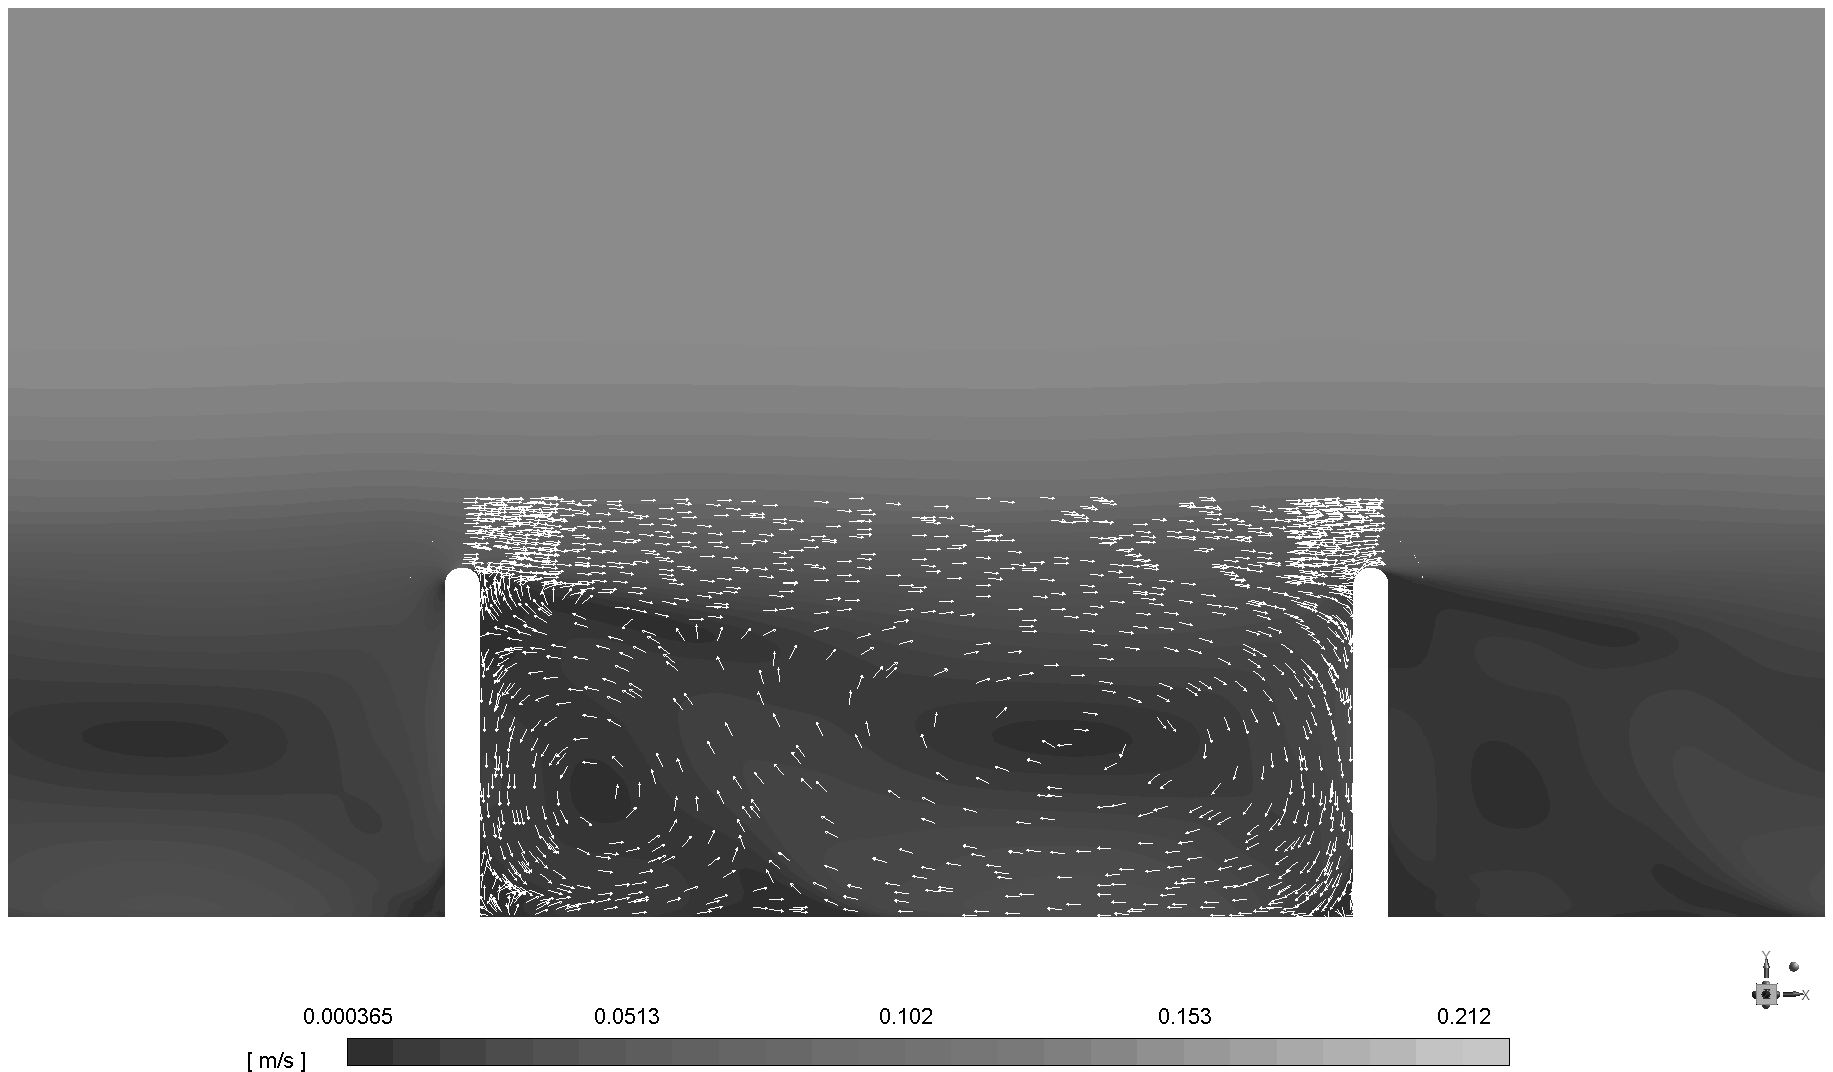
\includegraphics[width=\linewidth]{../images/art1/imgMassExchange3.png}
\caption{Mean velocity contour.}
\label{fig:art1:contour}
\end{figure}

Figure \ref{fig:art1:graphs} shows the mean streamwise velocity distributions for x/L = 0.25, 0.50 and 0.75 (x has origin in the right face of the first groyne and points to the right). Overall, the model had a good accordance in the main channel and in the central part of the groyne field. The computational model was able to capture the circulation pattern inside the groyne field. However, near the groyne heads (interface between the main channel and the groyne fields) the concordance was not so good. This is due to the high dissipation of momentum that occurred in the mixing layer. Despite the fine resolution of the grid, the model could not describe the flow inside this region. For the same reason the secondary gyre did not have contact with the mixing layer, since this vortex was formed by the dissipation of momentum from the primary gyre. The mean error was approximately 102\%, 21 \% and 47 \% for Figure \ref{fig:art1:graphs} a), b) and c), respectively. However, the flow was in the same order of magnitude than the experimental, which indicates that (Figure \ref{fig:art1:contour}) represents qualitatively, at least, the flow within the region.

The ejection of tracer from a groyne field to the mixing layer (region between the DWZ and the main channel) occurs in the upstream portion of the field (up to 40\%), while the following 60\% is a region where mass can re-enter the system \cite{weitbrecht2004}. The tracer concentration stayed higher in the secondary gyre, while the primary gyre oscillated due to the injection of tracer from the mixing layer and its natural ejection (Figure \ref{fig:art1:tracerContour}). This movement was captured by the model and can be seen completely in https://youtu.be/9b-4JZJdeA0.

\begin{figure}[!ht]
\centering
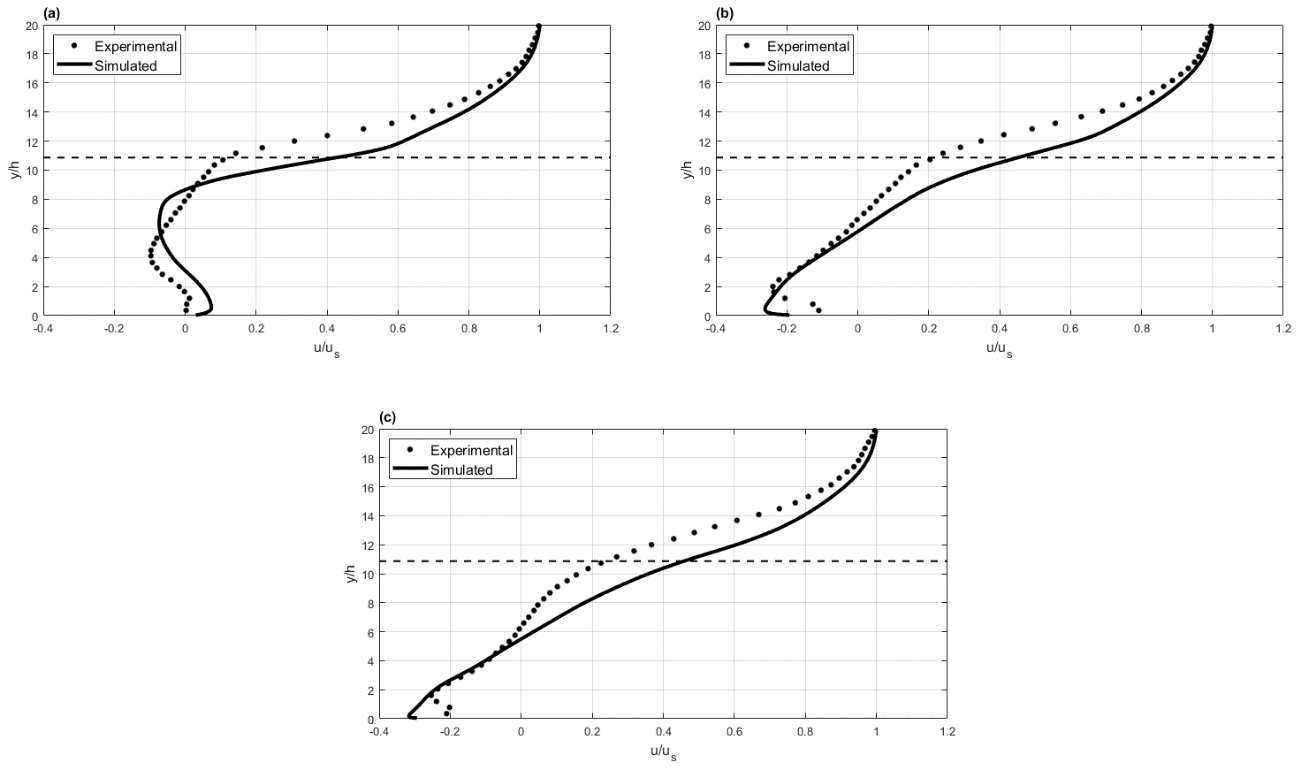
\includegraphics[width=\linewidth]{../images/art1/imgMassExchange4.png}
\caption{Mean streamwise velocity distributions. a) x/L = 0.25 b) x/L = 0.50 and c) x/L = 0.75. The dashed line represents the groyne head position (y/h = 10.87).}
\label{fig:art1:graphs}
\end{figure}
\begin{figure}[!ht]
\centering
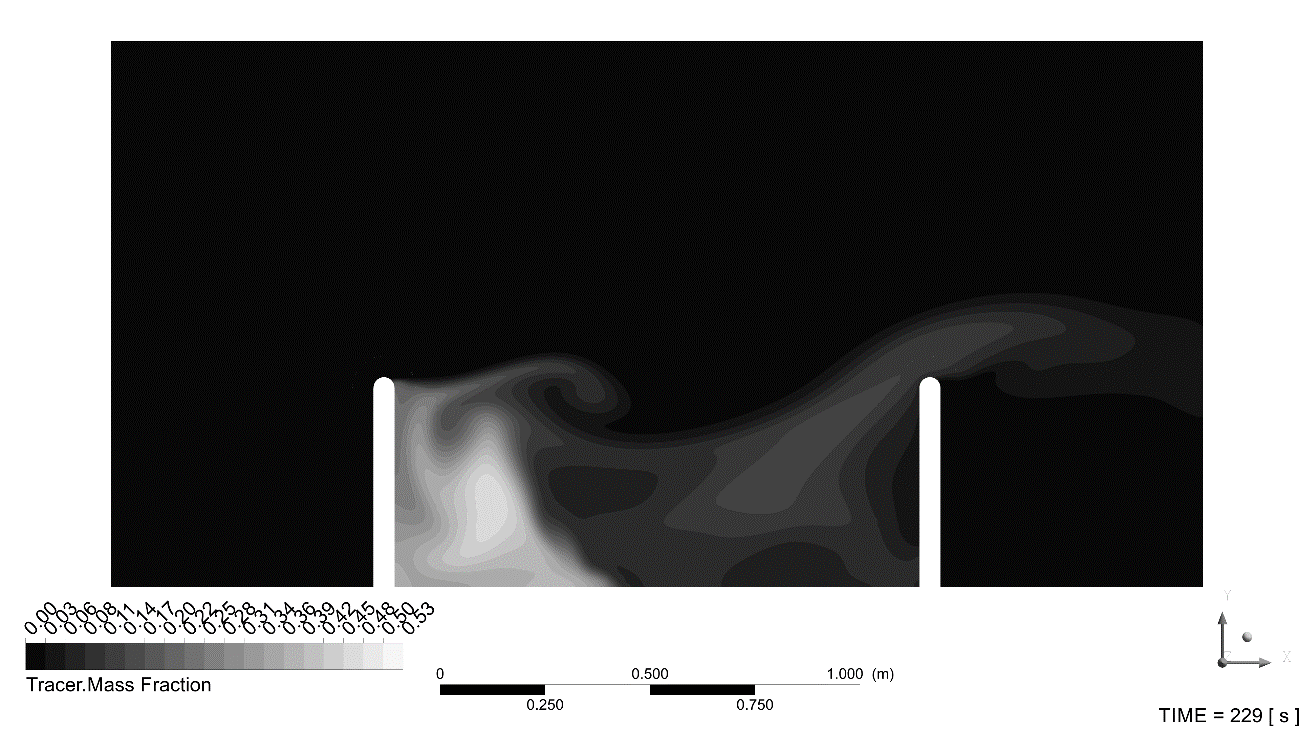
\includegraphics[width=\linewidth]{../images/art1/imgMassExchange5.png}
\caption{Tracer mass fraction in the free-surface plane in time 229s.}
\label{fig:art1:tracerContour}
\end{figure}

The tracer concentration inside the field was fitted in a first order decay model (Equation \ref{eqn:art1:massDecay}) following the same procedure from the experimental study (Figure \ref{fig:art1:massGraph1}).
\begin{equation}
C=C_0 e^{\frac{-t}{MRT}}
\label{eqn:art1:massDecay}
\end{equation}
Where MRT is the mean retention time. Based on the MRT, the mass coefficient k (Equation \ref{eqn:art1:k}) was calculated in order to estimate the intensity of mass exchange \cite{weitbrecht2001}.
\begin{equation}
k=\frac{W}{MRT U}
\label{eqn:art1:k}
\end{equation}The fitted curve presented an $MRT = 117.7s$ that related to an exchange coefficient of $k = 0.026$. The relative error between the mean value of Weitbrecht’ experiments and our model was 1.99\% for the exchange coefficient and 1.69 \% for MRT (Table \ref{tab:art1:kVal}).

Although we could observe a good fitting between our computational model and the experimental results, it can be observed that the system presented two slopes, with a breakpoint near $C/C0 = 0.2$ (Figure \ref{fig:art1:massGraph1}). The first slope was influenced by the tracer concentration present in the primary gyre, that oscillates between ejecting mass and re-absorbing via the shear layer. The second one ejects mass slower, as the concentration in the field was mainly disposed in the secondary gyre. Figure \ref{fig:art1:massGraph2} shows the tracer concentration fitted in two curves, the first curve presented an $MRT = 113.27s$ and a $k = 0.0274$ while the second $MRT = 121.43s$ and $k = 0.0256$. The summary of the model and comparisons with previous studies can be seen in Table \ref{tab:art1:kVal}.

Our results are consistent with field observations. \textcite{sukhodolov2014}, for example, observed that the mass concentrated in the secondary gyre, since it presented the slowest velocities in the groyne field.

\begin{figure}[!ht]
\centering
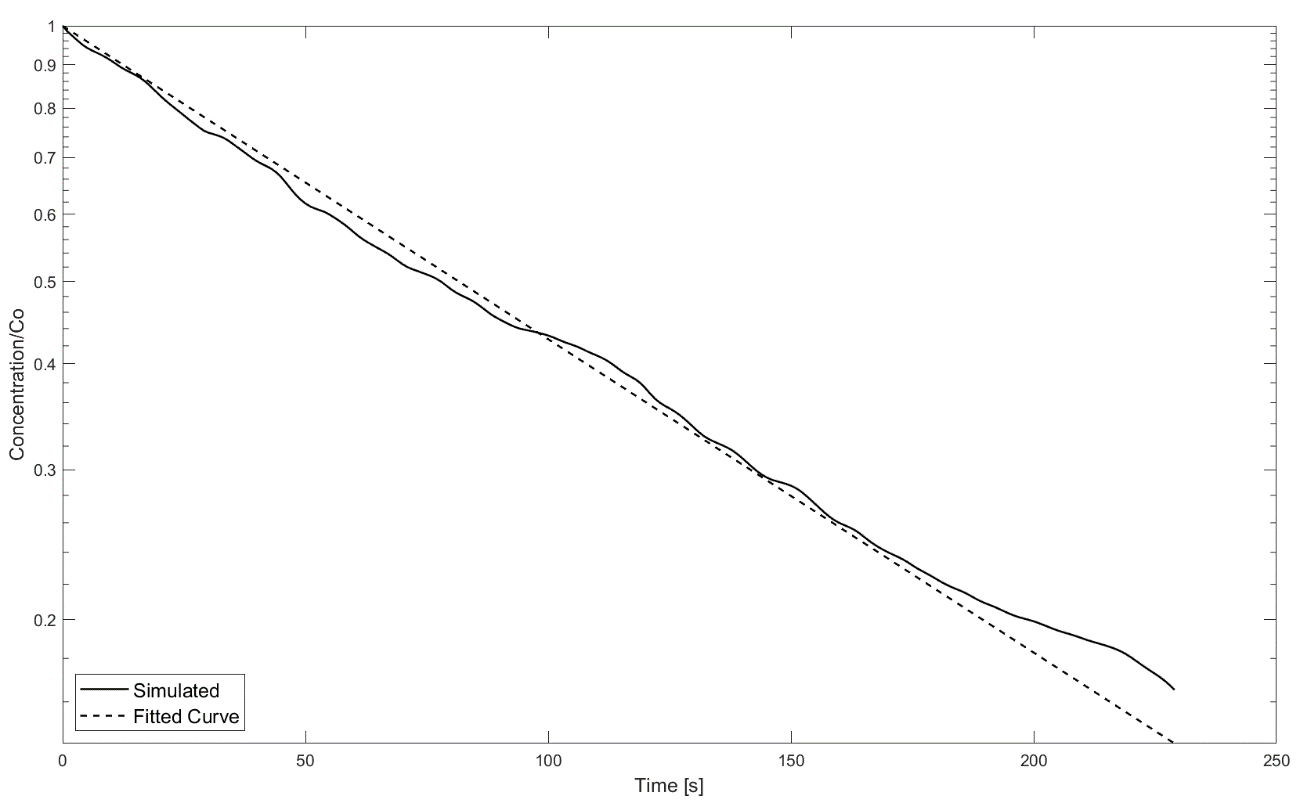
\includegraphics[width=\linewidth]{../images/art1/imgMassExchange6.png}
\caption{Volumetric averaged mass concentration inside groyne field.}
\label{fig:art1:massGraph1}
\end{figure}
\begin{figure}[!ht]
\centering
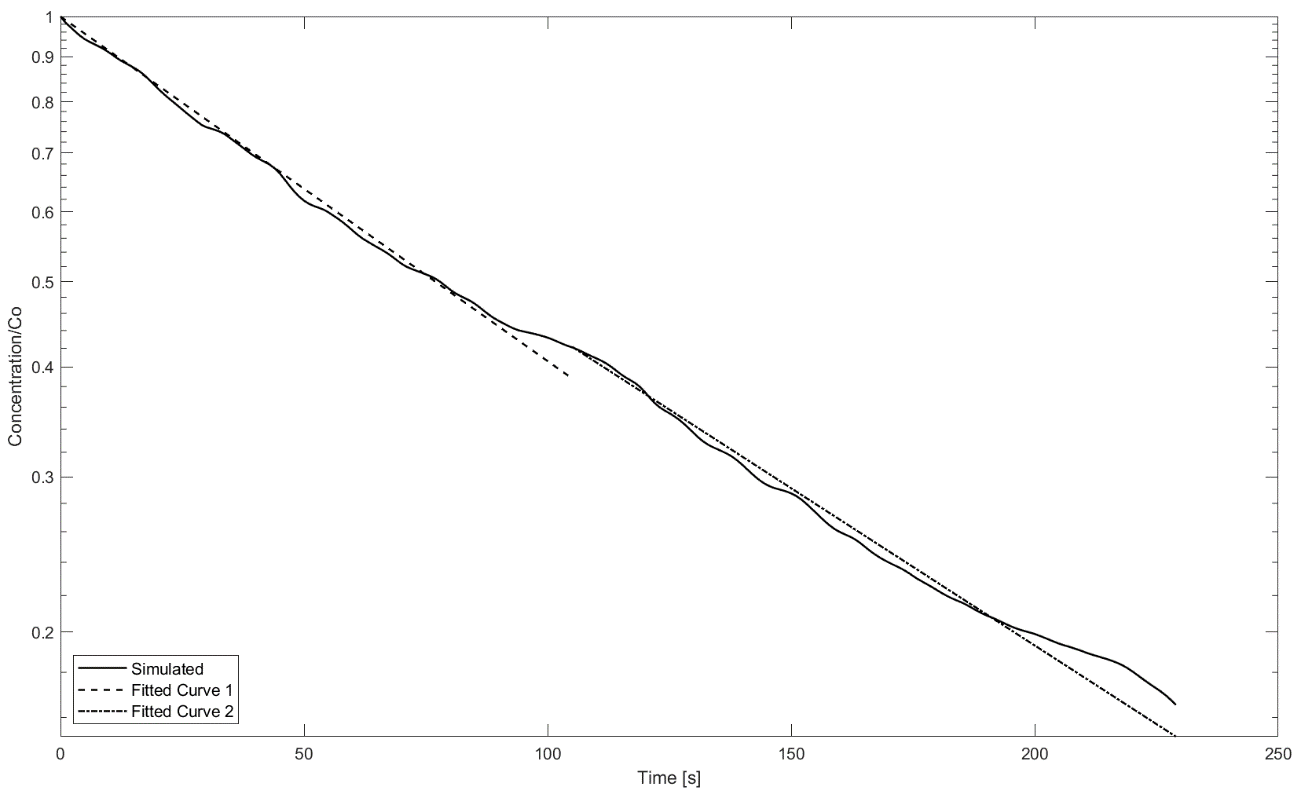
\includegraphics[width=\linewidth]{../images/art1/imgMassExchange7.png}
\caption{Volumetric averaged mass concentration inside groyne field fitted with two curves.}
\label{fig:art1:massGraph2}
\end{figure}
\begin{table}[]
\centering
\caption{Comparison of mean residence time inside groyne field and exchange coefficient in between experimental and numerical studies.}
\label{tab:art1:kVal}
\begin{tabular}{lll}
Experiment/Model                     & MRT {[}s{]} & k      \\ \hline
Experiment 1                         & 97          & 0.029  \\
Experiment 2                         & 114         & 0.028  \\
Experiment 3                         & 125         & 0.022  \\
Mean value of experiments            & 118         & 0.027  \\
3D LES \textbackslash{}cite\{Hinterberger2007\}                                            & 137 & 0.023 \\
\begin{tabular}[c]{@{}l@{}}2D LES \textbackslash{}cite\{\\ Hinterberger2007\}\end{tabular} & 75  & 0.042 \\
3D k-omega SST (global fitted curve) & 117.7       & 0.026  \\
3D k-omega SST (first slope)         & 113.3       & 0.0274 \\
3D k-omega SST (second slope)        & 121.62      & 0.0256 \\ \hline
\end{tabular}
\end{table}

\section{Conclusion}
A 3D k-omega SST simulation was presented for a periodic shallow water flow in a groyne field. Out model was able to reproduce a similar structure and magnitude flow compared to experimental data. Furthermore, our model could predict the mass exchange coefficient between the main channel and the DWZ and the mean retention time of the DWZ, being in good concordance with experimental results. In agreement to experimental and field observations, the decay of mass inside the field is described in two phases, first when the primary gyre dominates the ejection and second when the mass in concentrated in the second gyre prolonging the MRT. Hence, a simpler model than LES can predict the main parameters related to the mass exchange process in groyne structures.

%\nomenclature{$h$}{Flow Depth\nomunit{$m$}}
%\nomenclature{$B$}{Experimental channel width\nomunit{$m$}}
%\nomenclature{$W$}{Groyne field width\nomunit{$m$}}
%\nomenclature{$L$}{Groyne field length\nomunit{$m$}}
%\nomenclature{$U$}{Mean streamwise velocity in the main channel\nomunit{$m/s$}}
%\nomenclature{$tke$}{Turbulent kinetic energy\nomunit{$m^2/s^2$}}
%\nomenclature{$\omega$}{Specific dissipation rate\nomunit{$1/s$}}
%\nomenclature{$\rho$}{Fluid mass density\nomunit{$kg/m^3$}}
%\nomenclature{$Y_i$}{Local mass fraction of each species}
%\nomenclature{$D_{i,m}$}{Mass diffusion coefficient for the species in the mixture}
%\nomenclature{$\vec{v}$}{Velocity vector\nomunit{$m/s$}}
%\nomenclature{$Sc_t$}{Turbulent Schmidt number}
%\nomenclature{$\mu_t$}{Turbulent viscosity\nomunit{$kg/m s$}}
%\nomenclature{$D_t$}{Turbulent diffusivity\nomunit{$m^2/s$}}
%\nomenclature{$C$}{Concentration}
%\nomenclature{$MRT$}{Mean retention time\nomunit{$s$}}
%\nomenclature{$t$}{Time\nomunit{$s$}}
%\nomenclature{$k$}{Mass exchange coefficient}
%\printnomenclature

\addcontentsline{toc}{section}{Acknowledgements}
\section*{Acknowledgements}
The authors are grateful to members of SCF laboratory for providing the necessary hardware. Specially, D.F. Silva, M.L.M. Xavier, P.H.S de Lima, T.C.R Ventura and T.N. Yamasaki for research assistance and hardware set up.

\addcontentsline{toc}{section}{Funding}
\section*{Funding}
This study was financed in part by the Coordenação de Aperfeiçoamento de Pessoal de Nível Superior - Brazil (CAPES) -Finance Code 001.
\addcontentsline{toc}{section}{References}
\printbibliography[segment=\therefsegment,heading=subbibliography, title={References}]
\chapter{Hydrodynamics of Vegetated Lateral Cavities}
\label{chap:art2}
In this chapter, the second topic of the dissertation is presented as a published conference paper. This paper was originally written in Portuguese and was translated for this dissertation. The objective of this paper was to develop a simple numerical method capable of estimating the flow and the mass exchange between a lateral cavity and the main channel. 

The original paper was published in the '17º Congresso Nacional do Meio Ambiente', on September 24th 2020, Poços de Caldas, Brazil.
\section*{Authors}
\begin{itemize}
    \item Luiz Eduardo Domingos de Oliveira \footnote{Federal University of Mato Grosso do Sul}
    \item Taís Natsumi Yamasaki \footnotemark[1]
    \item Felipe Rezende da Costa \footnotemark[1]
    \item Johannes Gérson Janzen \footnotemark[1]
    \item Carlo Gualtieri \footnote{University of Naples Federico II}
\end{itemize}
\addcontentsline{toc}{section}{Abstract}
\section*{Abstract}
In rivers and channels, dead zones are regions of low velocity with the presence of recirculation motion, that have important ecological functions (eg. sediment retention) and also can be formed from human-made structures (eg. transversal dikes). The presence of vegetation in dead zones is a new topic of this discussion opening its way in the vegetated flow area of study, as the vegetation has the potential of changing the flow and altering mass exchange processes with the main channel. This study aimed to develop a numerical model of a single vegetated lateral cavity using Computational Fluid Dynamics (CFD). The vegetation drag was represented by a porous media which coefficients were calculated from experimental data. The results of the model shown that the cavity had a single vortex system in its interior and the flow velocity varied from $-0.11$ to $ 0.24 cm/s$. The simulation adapted well to the experimental data, which proved that the porous media is a suitable method of representing the vegetation drag in CFD.

\noindent\textbf{Keywords:} Lateral Cavities; Vegetation; Computational Fluid Dynamics (CFD).

\section{Introduction}
Rivers are formed by complex morphological boundaries, that create a variety of regions of high or low flows. One of these regions is named dead zone, in which slow velocities occur when compared to the main channel. The dead zones can occur naturally through lateral cavities \cite{jackson2013} or in man-made structures, groyne fields \cite{sukhodolov2017} and transversal dikes \cite{Pandey2018}. From the environmental point of view, dead zones function a 'foam' that absorbs part of the energy from the flow, which causes it to favour the retention of sediments, the protection of the margins and creates a habitat for biota that depends on slow waters \cite{Weitbrecht2008}.

In the field of vegetated flows, in which the main objective is to study the hydrodynamics between the flow and the vegetation, the research of vegetated dead zones is still recent. The presence of vegetation in the dead zone offers an additional drag to the flow, further impacting the velocity patterns in the region. Henceforth, the mass exchange processes between the main channel and the dead zone are also altered \cite{xiang2019}. This enlightens the importance of understanding the relationships, so it could be better used aiming to benefit the surrounding ecosystem. This study aims to simulate through Computational Fluid Dynamics (CFD) a vegetated lateral cavity using a porous media to represent the vegetation.

\section{Methods}
The chosen geometry consisted of a part of a channel and a lateral cavity (Figure \ref{fig:art2:compDomain}) based in \cite{xiang2019}. The depth of the flow and the channel ($H$) was defined in $0.10\,m$ and the channel width ($B$) in $0.30\,m$. The cavity was $L=0.25\,m$ long and $W=0.15\,m$ wide. The mean velocity was kept constant as $U=0.101\,m/s$, which corresponded to a Reynolds number of $Re=9000$ (turbulent flow). The water was kept at a constant temperature of $T=293$ K.

\begin{figure}[!ht]
\centering
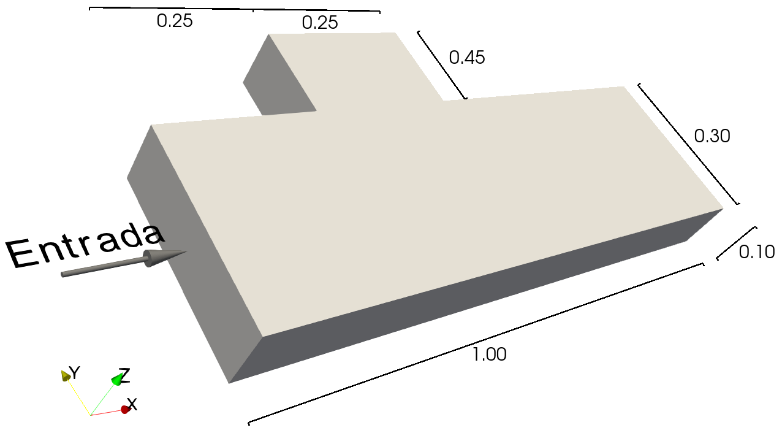
\includegraphics[width=\linewidth]{../images/art2/imgHyd1.png}
\caption{Computational domain. The flow direction is indicated by the grey arrow ('Entrada'). The dimensions are in metres and the coordinate origin ($x, y, z = 0$) at the lower right portion of the channel.}
\label{fig:art2:compDomain}
\end{figure}
The used boundary conditions were a longitudinal plane that cuts the domain at $y=0$ and at the top of the domain ($z=0.10$ m) that were defined as slip surfaces. The planes that cut the left portion of the channel and the cavity walls were considered hydraulic smooth walls of zero velocity. The channel entrance ($x=0\,m$) imported a velocity profile previously simulated in a periodic channel. The outlet surface ($x=1.00\,m$) was calculated with a zero gradient function.

The vegetation was represented with a porous media that filled all the lateral cavity. This is a simple way to represent the vegetation drag, and yet being an effective method of capturing the hydrodynamic effects \cite{Yamasaki2019}.  The adopted porous media was calculated by the Darcy-Forchheimer model (DF), that divides the drag into viscous and inertial resistances. The coefficients were calculated using the Ergun formulation and \textcite{Sonnenwald2017}, the vegetation parameters used to calculate the coefficients for the DF were taken from the second case of \textcite{xiang2019}. The details of the used methods can be found in the user's guide of \textit{Fluent}\textsuperscript{\textregistered}.

The numerical model was simulated under the commercial software \textit{Fluent}\textsuperscript{\textregistered} (version 14), using the method of finite volumes to discretise the governing equations of mass conservation and momentum. The turbulence model applied was the Detached Eddy Simulation, with the contour model using the k-omega Shear Stress Transport. The simulation ran under a transient configuration for 350 seconds, that was enough time to stabilise the flow.
\section{Results and Discussion}
As expected, the flow inside the cavity became slower when compared to the main channel, the x component of the velocity varied between $0.11$ and $0.25U$ (Figure \ref{fig:art2:velCont}). The high-velocity gradient in the cavity entrance ($y=0.30\,m$) formed a shear layer that originated the vortexes. These vortexes were carried inside the cavity where a single circulation system, concentrated to the right portion, occurred as the streamlines in Figure \ref{fig:art2:velCont} indicates. The adjusted drag coefficients were: $83.37\,m^2$ for the viscous resistance and $3.79\,m^{-1}$ for the inertial resistance.

\begin{figure}[!ht]
\centering
\begin{subfigure}{0.49\textwidth}
  \centering
  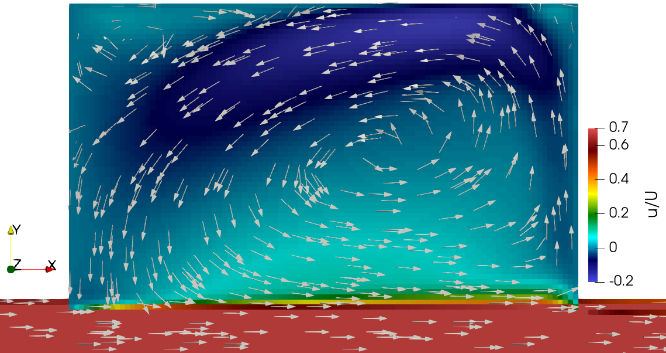
\includegraphics[width=0.9\linewidth]{../images/art2/imgHyd2.png}
  \caption[width=0.9\linewidth]{Contour and streamlines of the mean x-velocity.}
  \label{fig:art2:velCont}
\end{subfigure}%
\begin{subfigure}{.49\textwidth}
  \centering
  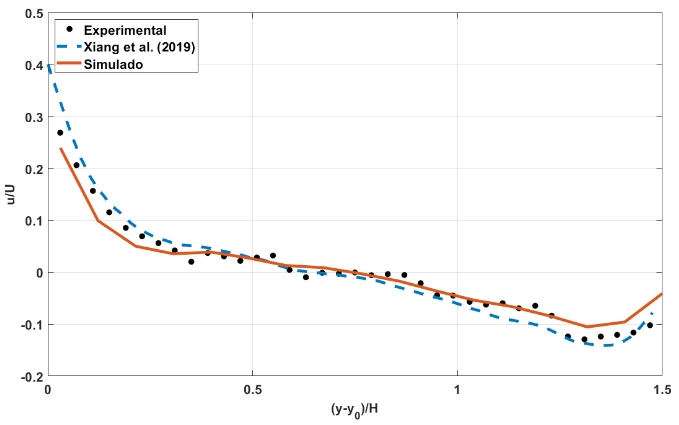
\includegraphics[width=0.9\linewidth]{../images/art2/imgHyd3.png}
  \caption[width=0.9\linewidth]{Mean velocity profile considering only the region inside the cavity.}
  \label{fig:art2:velProf}
\end{subfigure}
\caption{Velocity distributions along the plane $z=0.60H$.}
\label{fig:art2:velz06H}
\end{figure}
The y-velocity data was extracted along the plane $z=0.6H$ and condensed in a line using an ensemble averaging procedure along the y-axis similar to the procedure adopted in \textcite{sukhodolov2014}. The velocity profile is shown and compared with numerical and experimental data extracted from the literature in the Figure \ref{fig:art2:velProf}. At the entrance of the cavity ($(y-y_0)/H = 0$), the velocity $u$ was $0.25U$ and it kept getting slower as it moved towards the interior of the cavity. In $(y-y_0)/H = 1.4$, the flow got a negative value of $u = -0.1U$, indicating the presence of vortexes. The presented model, in orange, was well adjusted to the experimental data (black dots). This means that the porous media coefficients were well calculated and the model was capable of reproducing the flow in a accordance to the laboratory experiments.

\section{Conclusion}
The porous media model was capable of representing the vegetation in the numerical simulation. The cavity presented a single circulation system with a slower velocity than the main channel. The velocity profile obtained from the simulation was well adjusted to the experimental data, which further demonstrates that the model was capable of capturing the effects of vegetation inside the cavity.

%\nomenclature{$H$}{Flow Depth\nomunit{$m$}}
%\nomenclature{$B$}{Experimental channel width\nomunit{$m$}}
%\nomenclature{$W$}{Lateral cavity width\nomunit{$m$}}
%\nomenclature{$L$}{Lateral cavity length\nomunit{$m$}}
%\nomenclature{$U$}{Mean streamwise velocity in the main channel\nomunit{$m/s$}}
%\nomenclature{$Re$}{Reynolds number}
%\nomenclature{$T$}{Temperature\nomunit{$K$}}
%\printnomenclature

\addcontentsline{toc}{section}{Funding}
\section*{Funding}
This study was financed in part by the Coordenação de Aperfeiçoamento de Pessoal de Nível Superior - Brazil (CAPES) -Finance Code 001.
\addcontentsline{toc}{section}{References}
\printbibliography[segment=\therefsegment,heading=subbibliography, title={References}]
\chapter{Velocity Estimatives in Vegetated Lateral Cavities}
\label{chap:art3}
In this chapter, the second topic of the dissertation is further developed in a published conference paper. The objective of this paper was to develop a simple numerical method capable of estimating the flow and the mass exchange between a lateral cavity and the main channel. Differently of the previous chapter, this paper introduces an open source approach to the problem, making the model further accessible to the general public. Also, the numerical model was further developed to account the mass transfer between the regions.

The original paper was published in the 'XIII Encontro Nacional de Águas Urbanas', on October 2020, Porto Alegre, Brazil.
\section*{Authors}
\begin{itemize}
    \item Luiz Eduardo Domingos de Oliveira \footnote{Federal University of Mato Grosso do Sul}
    \item Taís Natsumi Yamasaki \footnotemark[1]
    \item Johannes Gérson Janzen \footnotemark[1]
    \item Carlo Gualtieri \footnote{University of Naples Federico II}
\end{itemize}
\addcontentsline{toc}{section}{Abstract}
\section*{Abstract}
Lateral cavities are a type of transient storage zones that occur in riverine systems. They play an important role in mass transport processes, especially due to a higher residence time. In this study, a numerical simulation of flow past a lateral cavity with vegetation was performed to assess the impact of the vegetation on the cavity hydrodynamics. The vegetation drag was introduced in a simplified method, as it was modelled as an anisotropic porous medium. The model could reproduce the experimental results at a reduced computational cost and can be considered a study platform for future studies.

\noindent\textbf{Keywords:} Lateral Cavities; Vegetation; Computational Fluid Dynamics (CFD).

\section{Introduction}

\addcontentsline{toc}{section}{References}
\printbibliography[segment=\therefsegment,heading=subbibliography, title={References}]

\chapter{The effects of vegetation density upon flow and mass transport in lateral cavities}
\label{chap:art4}
In this chapter, the main topic of this dissertation is developed. The effects of vegetation on the hydrodynamics and the mass exchange between the main channel/dead zone are investigated. The objective of this paper was to describe and possibly find a threshold on the behaviour of the dead zone given a certain density level.

\section*{Authors}
\begin{itemize}
    \item Luiz Eduardo Domingos de Oliveira \footnote{Federal University of Mato Grosso do Sul}
    \item Taís Natsumi Yamasaki \footnotemark[1]
    \item Filipe de Lima Queiroz \footnotemark[1]
    \item Felipe Rezende da Costa \footnotemark[1]
    \item Johannes Gérson Janzen \footnotemark[1]
    \item Carlo Gualtieri \footnote{University of Naples Federico II}
\end{itemize}

\addcontentsline{toc}{section}{Abstract}
\section*{Abstract}
Lateral cavities are regions attached to rivers affect the flow by creating a dead water zone. These regions reduce the flow velocity increasing the deposition of sediment and the temporary storage of polluted materials, which favours the growth of aquatic vegetation. The effect of this vegetation growth was studied using different vegetation densities in a Large Eddy Simulation (LES). The vegetation drag was represented by a porous media calculated with the Darcy-Forchheimer model. This numerical model showed that the hydrodynamics of the flow can present different patterns and phases for a vegetation density $0<a(\%)<10.656$. Furthermore, the occurrence of a secondary circulation was found where it normally would not occur for a non-vegetated scenario.

\noindent\textbf{Keywords:}: Lateral Cavity; Aquatic Vegetation; Mass Exchange; Computational Fluid Dynamics (CFD).

\section{Introduction}
Lateral cavities are an important component of riverine \cite{Harvey2015} and estuarine \cite{Ward1984} systems, because they (1) function as a macro-roughness at the river banks \cite{juez2017}, (2) drive mass exchange processes with the open channel \cite{Ouro2020, Mignot2017,jackson2015}, (3) act as transient storage zones \cite{jackson2015,drost2014,jackson2013a}, and (4) enhance biodiversity in the system \cite{harvey2016,ribi2014,Watts2004}. These functions are linked to morphology-induced flow heterogeneity \cite{jackson2013a,Sanjou2012,Meile2011}. Drawing on studies that demonstrated the relevance of transient storage zones on nutrient retention and cycling \cite{Ensign2005, Mulholland1994}, lateral cavities can play a role in these processes because of increased timescales of solutes, especially due to the formation of recirculation gyres \cite{jackson2012,Gooseff2005}. In face of flushing events, mobilized sediment can be carried out of the cavities, which may pose a risk of releasing pollutants in the stream \cite{Forrest2007}.

In aquatic systems, the retention of fine sediments and nutrients constitutes a favourable substrate for vegetation establishment and growth \cite{Nepf2012,Vandenbruwaene2011,Asaeda2009,Cotton2006,Barko1991}, which occurs in lateral cavities and embayments \cite{Jones2020,Ely2010,Olesen1996,Ward1984}. Except to the case of invasive species \cite{Maceina1999}, vegetation serves to refuge and sustain fish communities \cite{Kraus2012,Arend2008}, trap suspended material \cite{Ward1984} and protect from bank erosion \cite{Duro2020}, these two last features being associated with the ability of vegetation to dissipate flow energy. Consequently, vegetation canopies increase the retention time and are considered by some authors as transient storage zones by themselves \cite{Kurz2017}.

The hydrodynamics of vegetated cavities are mainly dependent on the incoming flow properties, cavity geometry and vegetation characteristics \cite{xiang2020,xiang2019,Lu2016,sukhodolov2017}. \textcite{xiang2019} showed that the degree of vegetation effects on the initial bare-bed cavity depends on the vegetation density. The authors tested five vegetation densities in a rectangular cavity, using Computational Fluid Dynamics (CFD). The immediate effect of increasing the density was a reduction in velocity magnitude and turbulence inside the cavity, which was caused by the flow resistance exerted by the vegetation. The interface connecting the cavity to the channel presented a mixing layer with higher turbulence and vorticity than the rest of the domain, as a consequence of von Karman vortex streets generated by the vegetation, combined with shedding vortices created at the entrance corner of the cavity. Further, secondary recirculation gyres in the cavity were suppressed by denser vegetation values.

Field-scale experiments performed by \textcite{sukhodolov2017} at a vegetated groyne (a type of cavity that is built inside the open channel, according to \textcite{jackson2013}), indicated that denser vegetation diffused more momentum from the jet coming at the groyne entrance, which modified the circulation patterns in the groyne. The experiments showed that vegetation imposed a single circulation in the groyne, similar to \textcite{xiang2019}, but that vegetation had little effect on the mixing layer formed at the groyne-channel interface. Another difference between the two studies was that \textcite{sukhodolov2017} found that the emergent vegetation induced uniform flow patterns along with the depth, whereas \textcite{xiang2019} indicated that the flow pattern specifically at the cavity interface changes with depth in the presence of vegetation. Moreover, \textcite{xiang2020} showed that vegetation blocked the development of the mixing layer spreading inside the groyne, which affects the exchange between the open channel and the cavity (denser vegetation blocks more flow) and increases the mean retention time of the flow in the cavity, for denser vegetation \cite{xiang2019}.

The studies with vegetated cavities, as described above, varied the vegetation density between 0 and 0.627\% \cite{xiang2019}, 0 and 0.969\% \cite{xiang2020}, and 1.57\% \cite{sukhodolov2017}. Experimentally, \textcite{xiang2020} mentioned the difficulty to test denser vegetation arrays in cavities because the array would block the laser light and, thus, compromise flow measurements. The authors expanded the density values using numerical simulations. However, a reference threshold for vegetation to be considered “dense” or “sparse” in cavities has not been defined to date, and it points to the need of understanding which density thresholds will cause key flow modifications in the cavity (e.g., the suppression of recirculation gyres, the complete suppression of flow, the exchange coefficient asymptote, etc.). For emergent vegetation patches in an open channel, \textcite{chen2012} characterized them as being “dense” or “sparse” according to flow blockage thresholds, in which the flow properties near the patch (e.g., flow adjustment length and the velocity exiting the patch) were distinct above and below the threshold. A similar approach can be done for vegetated cavities. Furthermore, in previous field and laboratory experiments \cite{Mignot2017,Constantinescu2009,weitbrecht2004,weitbrecht2001,Uijttewaal2001}, the mass exchange between the main channel and a dead water zone, lateral cavity or groyne, was studied with the ejection of tracer fields. This method of analysing the transport of the passive scalar provides a different perspective of the physics of this exchange and should be further explored \cite{xiang2019}. Hence, a dynamic model that considers passive scalar motion can be an effective way to help river managers to predict pollutant transport in accidental spills.

The objective of the present study was to expand the vegetation density range and identify the thresholds that can differentiate dense to sparse vegetation in a lateral cavity. The study was performed with CFD simulations.

This paper is divided into five main sections. Following the Introduction, the details of the numerical model were described, along with the grid independence test and solution quality. Third, the hydrodynamic characteristics of the flow were presented. Fourth, the impact on the mixing layer is presented and discussed. Fifth, the impact of the vegetation in the mass exchange is discussed. Finally, the conclusive remarks about the influence of vegetation in a single circulation lateral cavity were presented.

\section{Numerical Model}
\subsection{Model Equations}
The simulations were performed with the Large Eddy Simulation (LES) model, which uses the spatial filtering of the incompressible Navier-Stokes equations to solve the fluid motion and turbulence. For an incompressible fluid, the equations of mass and momentum conservation are depicted as follow, respectively:
\begin{equation}
\frac{\partial \bar{u}_i}{\partial x_i}=0  \left \{ i=1,2,3 \right \}
\label{eqn:art4:continuity}
\end{equation}
\begin{equation}
\frac{\partial \bar{u_i}}{\partial t}+\frac{\partial}{\partial x_j}(\bar{u}_i \bar{u}_j)=-\frac{1}{\rho}\frac{\partial \bar{p}}{\partial x_i}+\frac{\partial}{\partial x_j}\left [ \mu (2\bar{S}_{ij}) - \tau_{ij} \right ] + \bar{S}_{M,i}
\label{eqn:art4:NS}
\end{equation}

in which the overbar indicates resolved quantities; $\bar{u}_i$ (m/s) is the velocity component in the i direction ($i = 1, 2, 3$ correspond to x, y, z-axis, respectively), $\rho$ (kg/m³) is the fluid density, $\bar{p}$ (N/m²) is the dynamic pressure, $\mu$ (m²/s) is the kinematic viscosity, $\bar{S}_{ij}$ (1/s) is the strain-rate tensor, $\tau_{ij}$ (m²/s²) is the subgrid-scale stress, and $\bar{S}_{M,i}$ is the sink term related to vegetation drag (m/s²). $\bar{S}_{ij}$ and $\tau_{ij}$ are given by: 
\begin{equation}
\bar{S}_{ij}=\frac{1}{2}\left (\frac{\partial u_i}{\partial x_j} +\frac{\partial u_j}{\partial x_i} \right )
\label{eqn:art4:Sij}
\end{equation}
\begin{equation}
\tau_{ij}=\bar{u}_i\bar{u}_j - \overline{u_j u_i}
\label{eqn:art4:Tij}
\end{equation}
Specifically, $\tau_{ij}$ represents the effect of unresolved small-scale motion on the resolved flow, and is based on the eddy-viscosity assumption:
\begin{equation}
\tau_{ij} - \frac{1}{3}\tau_{kk}\delta_{ij}=\nu_t(2\bar{S})ij)
\label{eqn:art4:tau}
\end{equation}

where $\nu_t$ (m²/s) is the eddy viscosity. In this study, the Wall-Adapting Local Eddy-viscosity (WALE) model, proposed by \textcite{nicoud1999}, was chosen as the subgrid-scale model to calculate $\nu_t$.

Even for CFD, adding more rigid cylinders in the cavity in order to increase the density \cite{xiang2019,xiang2020} results in a heavier mesh that requires greater computational processing to run the model. The vegetation is considered uniform as flows like in lateral cavities are subject to riparian plants and vegetation cover that can develop almost uniformly of the area \cite{sukhodolov2017}. For these reasons, the present study proposed to use the Darcy-Forchheimer porous media approach to represent the vegetation, adjusting the resistance in the horizontal and vertical directions. The vegetation inside the cavity was represented by a porous media, in which the momentum loss caused by the vegetation drag was computed through the Darcy-Forchheimer (DF) model (Equation \ref{eqn:art4:DF}). 

\begin{equation}
\bar{S}_{M,i}=\left ( -\mu d+\frac{\rho\left | u_{jj} \right |}{2}f \right )u_i
\label{eqn:art4:DF}
\end{equation}

in which $d$ (1/m2) is the viscosity drag coefficient and $f$ (1/m) is the inertial coefficient. First, the porous model was configured and validated with laboratory experiments performed by \textcite{xiang2019}, who created a surrogate for rigid vegetation by displaying different arrays of copper wires for different vegetation density values in the cavity. Then, to expand the density range, simulations with higher density values were performed, assuming the same stem diameter of \textcite{xiang2019}. The wire diameter was $d_w = 0.15 cm$. The vegetation density, $a$, was calculated as follows:

\begin{equation}
a=\frac{n S_V}{S_{cav}}
\label{eqn:art4:a}
\end{equation}

in which $n$ is the number of vegetation stems, $S_V$ (m²) is the horizontal cross-section area of the stems, and $S_{cav}$ (m²) is the cavity area. The coefficients $d$ and $f$ were calculated using the Ergun equation:

\begin{equation}
d=\frac{150}{D_{p}^{2}}\frac{\left ( 1-\epsilon \right )^2}{\epsilon^3}
\label{eqn:art4:d}
\end{equation}
\begin{equation}
f=\frac{3.5}{D_{p}}\frac{\left ( 1-\epsilon \right )}{\epsilon^3}
\label{eqn:art4:f}
\end{equation}

in which $D_p$ (cm) is the mean particle diameter, and $\epsilon$ $(= 1-a)$ is the void fraction. In the horizontal direction (flow perpendicular to the stems, which corresponds to the \textit{x-} and \textit{y-}axis), $D_p$ was assumed as the wire diameter ($D_p = d_w$). To account for non-isotropic resistance, the approach of \textcite{oldham2001} was used to calculate $d$ and $f$ in the $z$-axis, where the flow is parallel to the stems. In this case, $D_p$ was calculated as the hydraulic diameter $d_h$ (cm): 

\begin{equation}
d_h=d\left ( \frac{4\left ( \frac{s}{d} \right )^2}{\pi} - 1\right )
\label{eqn:art4:dh}
\end{equation}

In which $s/d$ is the spacing: diameter ratio between the wires.

\subsection{Simulation Setup}
The numerical model was developed based on the physical experiments of \textcite{xiang2019}. The 3D geometry consisted of a single lateral cavity that was adjacent to a rectangular open channel Figure (\ref{fig:art4:domain}). The lateral cavity was $W=0.15$ m wide and $L = 0.25$ m long, resulting in the aspect ratio $W/L=0.60$, which falls in the range of $0.5\leq W/L\leq 0.15$ and thus corresponds to a one-gyre circulation system to be formed inside the cavity \textcite{Uijttewaal2001}. The depth of the channel and cavity was $H=0.10$ m. The flow in the main channel was turbulent ($Re=9000$) and subcritical ($Fr=0.102$), with bulk velocity $U = 0.101$ m/s at the channel inlet ($x=0$ m). The temperature was constant at $T=293K$.

\begin{figure}[!ht]
\centering
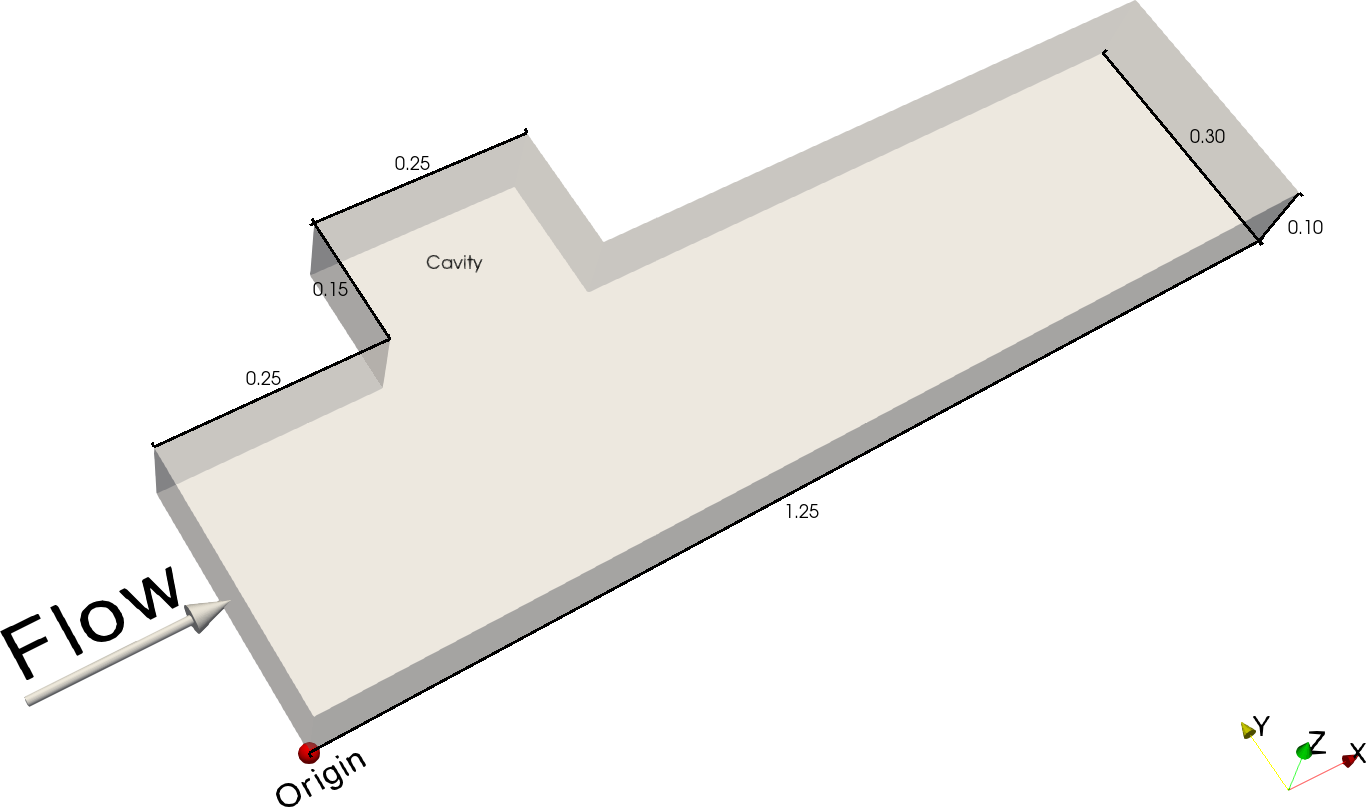
\includegraphics[width=\linewidth]{../images/art4/domain.png}
\caption{Computational domain with coordinates and dimensions.}
\label{fig:art4:domain}
\end{figure}

The boundary conditions set to the model were the following. The rigid-lid approximation was applied at the free surface of the domain ($z = 0.10$ m), which is valid for flows with $Fr < 0.5$ \cite{alfrink1983}. The longitudinal \textit{XZ} plane, located at $y=0$ m, where the main channel was restricted in the domain, was defined as a free-slip surface. Knowing that flow effects caused by obstacles to the main channel do not exceed one obstacle length \cite{Brevis2014}, and knowing that the cavity had $L=0.15$ m, we defined the width of the main channel to be $B=0.30$ m, which was sufficient to capture any flow effect in the main channel. The inlet portion of the domain ($x=0$ m) received precalculated velocity fields that were fully developed in a periodic channel, under the same flow conditions and the main channel geometry. The implementation of this boundary condition applied the turbulence Divergence-Free Synthetic Eddy Method (DF-SEM) to synthesise eddies based on the turbulence developed of the imported flow \cite{poletto2013}. A convective outflow boundary condition was adopted at the outlet ($x = 1.25$ m), in which the zero-gradient condition allows the flow to exit the domain without having any backflow. The bottom of the domain ($z = 0$ m) and the walls of the main channel ($y = 0.30$ m) and the cavity were considered as no-slip surfaces. 

The mass exchange between the main channel and the vegetated cavity was simulated with tracer fields, in which the washout procedure was implemented. After all the solution transients were eliminated, the lateral cavity was filled with an inert tracer. The flow was calculated until either all tracer left the cavity, or a time of 200 s passed. The associated turbulent Schmidt number was $S_{ct}=0.9$ , as used in other similar flows \cite{Gualtieri2017}. In this period, the average flow was, also, calculated and condensed into an ensemble averaging \cite{sukhodolov2014}. The computational time increment was held variable, with a Courant number kept under 0.90 and a maximum time step of 0.05 s.

The simulations were performed with the open-source package OpenFOAM (version 1912). To discretize the governing equations and numerical schemes, the module pimpleFoam, which employs the finite volume method (FVM), was used. For the pressure-velocity coupling, the PIMPLE method scheme was adopted. To solve the convection-diffusion equations, the implicit second-order backward time-stepping scheme and additional second-order schemes were used. The residual tolerance was set to $1 \times 10^{-4}$ and the number of our loops was set to 3, the same count was set for the pressure correction loops.

\subsection{Numerical Programme}
The study of the vegetated cavity was proposed by varying the vegetation density values using different DF coefficients to emulate the increasing drag, which is summarised in Table \ref{tab:art4:cases}. The density was varied between $a = 0$ (no vegetation) and $a = 10.656$\%, distributed in ten scenarios for simulation. The vegetation density found in natural conditions varies from $0.001<a<0.45$, and the effects of the turbulence dissipation remains predominant until  $a<0.1$ \cite{Nepf2012}, given that these values were based on a free open channel, we chose a smaller value of a that could comprehend all the turbulence dissipation spectrum as this is a key component of the hydrodynamics of dead waters. It was assumed that the vegetation was uniformly distributed in the cavity and that it spanned the cavity depth, similarly to emergent vegetation.

\begin{table}[]
\centering
\begin{tabular}{@{}lllllll@{}}
\toprule
\multirow{2}{*}{Case} & \multirow{2}{*}{a (\%)} & \multicolumn{2}{l}{Horizontal direction (x and y-axis)} & \multicolumn{3}{l}{Vertical direction (z-axis)} \\ \cmidrule(l){3-7} 
   &         & $d$ (1/m2)   & $f$ (1/m) & $dh$ (m) & $d$ (1/m2)  & $f$ (1/m) \\ \midrule
0  & 0       & 0.00       & 0.00    & 0.00   & 0.00      & 0.00    \\
1  & 0.1332  & 116.53     & 3.09    & 0.7624 & 0.000451  & 0.00608 \\
2  & 0.1665  & 182.25     & 3.87    & 0.8265 & 0.0006    & 0.00702 \\
3  & 0.3330  & 753.83     & 7.89    & 0.3902 & 0.0111    & 0.0303  \\
4  & 0.6660  & 3002.72    & 15.82   & 0.1846 & 0.198     & 0.19    \\
5  & 1.3320  & 12344.01   & 32.40   & 0.0836 & 3.98      & 0.58    \\
6  & 2.6640  & 51244.51   & 67.36   & 0.0360 & 88.96     & 2.81    \\
7  & 3.9960  & 120314.00  & 105.38  & 0.0210 & 613.12    & 7.52    \\
8  & 5.3280  & 223190.20  & 146.57  & 0.0139 & 2602.53   & 15.83   \\
9  & 7.9920  & 546724.99  & 239.43  & 0.0072 & 23702.83  & 49.85   \\
10 & 10.6560 & 1061150.94 & 348.58  & 0.0041 & 140829.09 & 126.99  \\ \bottomrule
\end{tabular}
\caption{Vegetation levels and the calculated Darcy-Forchheimer coefficients, where $a$ (\%) is the vegetation density, $d$ (1/m2) is the viscosity drag coefficient, $f$ (1/m) is the inertial coefficient and $dh$ (m) is the hydraulic diameter.}
\label{tab:art4:cases}
\end{table}
\subsection{LES Quality and Grid Independence}
The quality of the numerical solution was evaluated using a procedure based on three different grids \cite{Dutta2018}. The refinement rate between the grids was 1.80, although with the same configurations (numerical model and boundary conditions). The numerical and modelling errors were estimated and compared to the experimental data from \textcite{xiang2019}. Figure \ref{fig:art4:validation} shows the ensemble-averaged streamwise velocity with the total error (numerical and modelled) expressed by error bars. Overall, the numerical solution presented low error magnitudes, with a mean total error of –0.0024 m/s. The errors could be mitigated by a further refinement, although the errors were small enough to continue the experiments.

\begin{figure}[!ht]
\centering
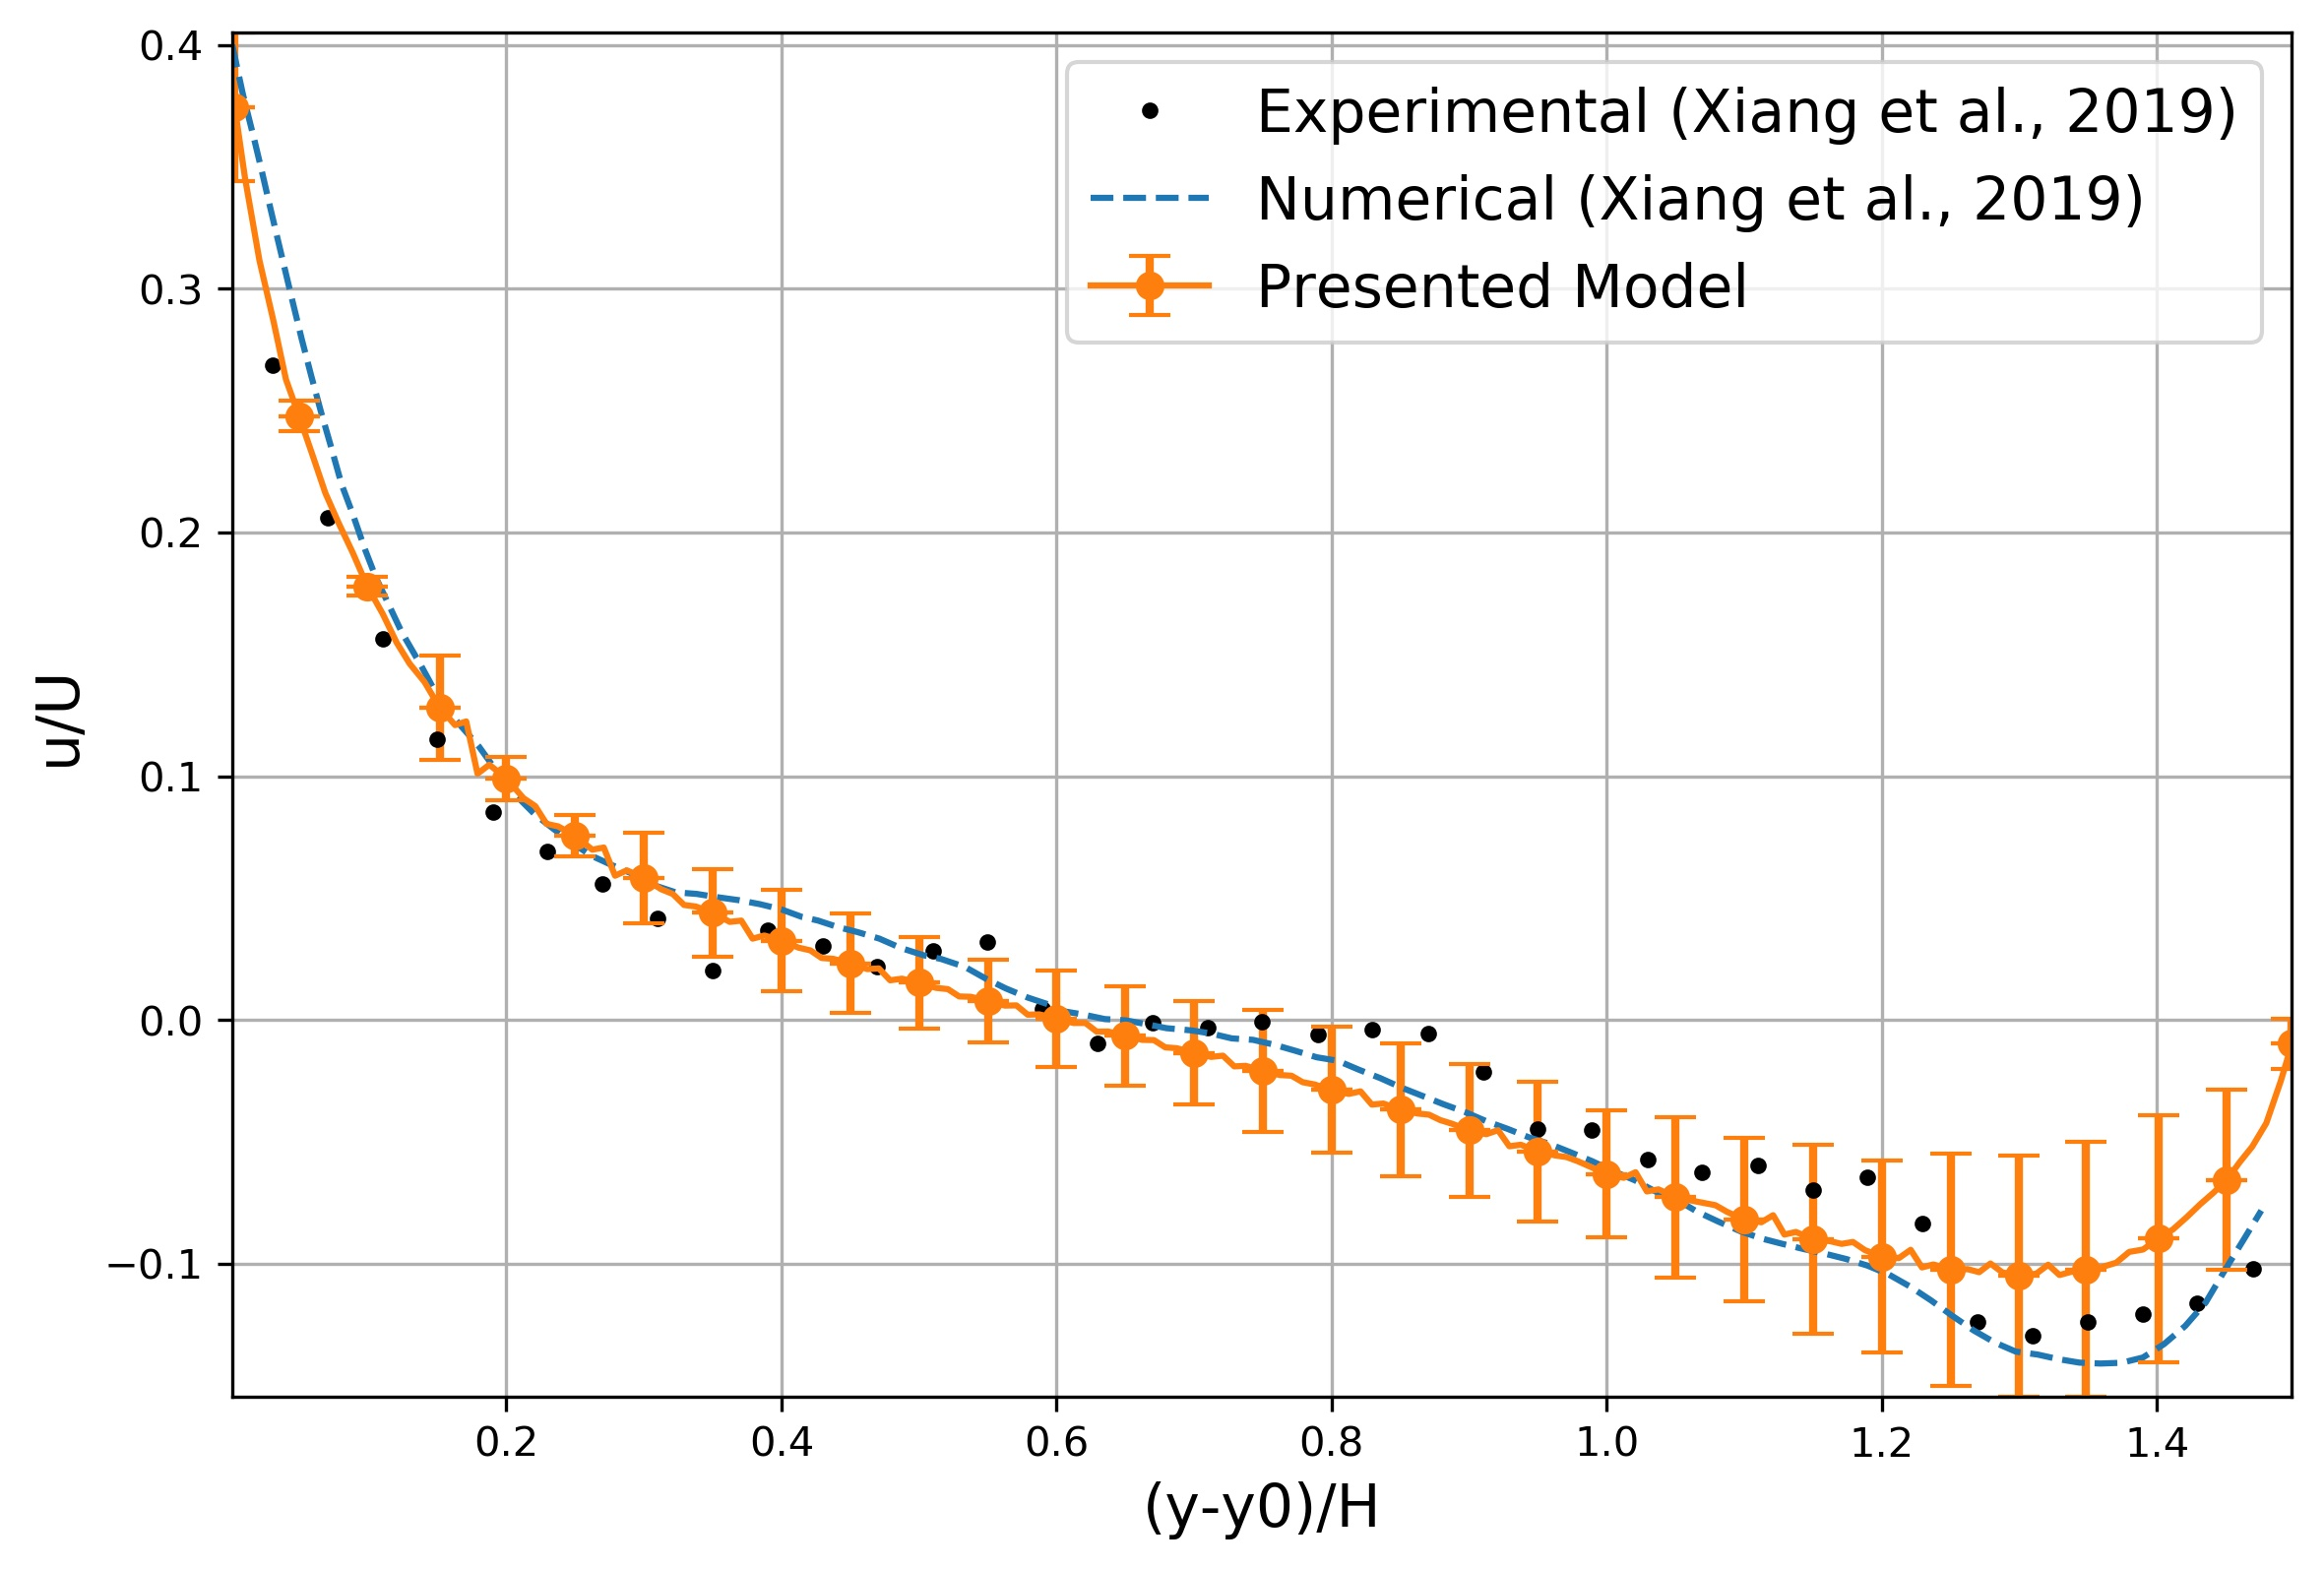
\includegraphics[width=\linewidth]{../images/art4/validation.jpeg}
\caption{Grid and Numerical Errors of the ensemble-averaged streamwise velocity in the cavity at $z=0.6H$, where $U$ is the bulk velocity in the main channel, $y_0=0.30$m represents the beginning of the cavity and $H$ is the height of the flow.}
\label{fig:art4:validation}
\end{figure}
\subsection{Validation}
Figure \ref{fig:art4:validation} compares the results of the time-averaged streamwise velocity \textit{u} at $z/H=0.6$ obtained from the second case ($a=0.1332$\%) of \textcite{xiang2019}, using both experimental and his numerical model. The numerical results, from the present paper, showed good consistency with the experimental data. A difference between the wall resolved LES (WRLES) and the wall modelled LES (WMLES) is highlighted in the region $(y-y_0)/H > 1.20$, where the continuous line deviated from the dashed result. Although, in all other regions the results followed closely both experimental and the WRLES.

\section{Flow Characteristics}
Figure \ref{fig:art4:velocityContour} show the mean 2D streamlines for all the cases at $z/H=0.6$. Under the cases 0 to 5 a main anti-clockwise motion takes place (Figure \ref{fig:art4:velocityContour}  a-f). The increase in vegetation density translates the centre of the gyre towards the main channel and downstream in the x-direction as the blockage effects increase and the flow loses energy faster. For $a=1.3320$\% (case 5) the main circulation starts to lose its shape and this process continues up to $a=3.9960$\% when the flow stabilised (Figure \ref{fig:art4:velocityContour}  f and Figure \ref{fig:art4:velocityContour}  g-h). The case 8 showed the formation of a secondary gyre system at the right portion of the cavity, $0.45<x/L<1$ and $0<y/W<1$ (Figure \ref{fig:art4:velocityContour}  i). This behaviour was shifted to the left as the vegetation increased to $a=7.9920$\% (Case 9), $0.30<x/L<1$ and $0<y/W<1$ (Figure \ref{fig:art4:velocityContour}  i). The presence of secondary circulations normally occurs at different aspect ratios: $W/L<0.5$ and $W/L>1.5$ \cite{Sukhodolov2002}, this circulation naturally does not have any contact with the main channel as they are derived from the primary circulation. Figure \ref{fig:art4:velocityContour}  i-k show the primary circulation at the bottom left of the cavity and the secondary gyre occupying approximately 50\% of the area in $a=5.3280$\%, the area comprehending the secondary gyre further increased with the vegetation drag increase.

Figure \ref{fig:art4:velXYPlane} show the flow at the horizontal plane \textit{XY} at $z/H = 0.6$ along the \textit{y}-axis, $(y-y_0)/H$ being $y_0=0.30$m the beginning of the cavity, where the velocity decreases as the vegetation density increases. Another important aspect of this figure is the positioning of the circulation centre that slowly shifts towards the region close to the interface ( $(y-y_0)/H=0$) that is associated with the flow resistance imposed by the vegetation.

\begin{figure}[!ht]
\centering
\includegraphics[width=\linewidth]{../images/art4/velocityContour.jpg}
\caption{Mean 2D streamlines of different vegetation densities at the horizontal plane $z/H = 0.6$: a) Case 0, b) Case 1, c) Case 2, d) Case 3, e) Case 4, f) Case 5, g) Case 6, h) Case 7, i) Case 8, j) Case 9 and k) Case 10.}
\label{fig:art4:velocityContour}
\end{figure}

\begin{figure}[!ht]
\centering
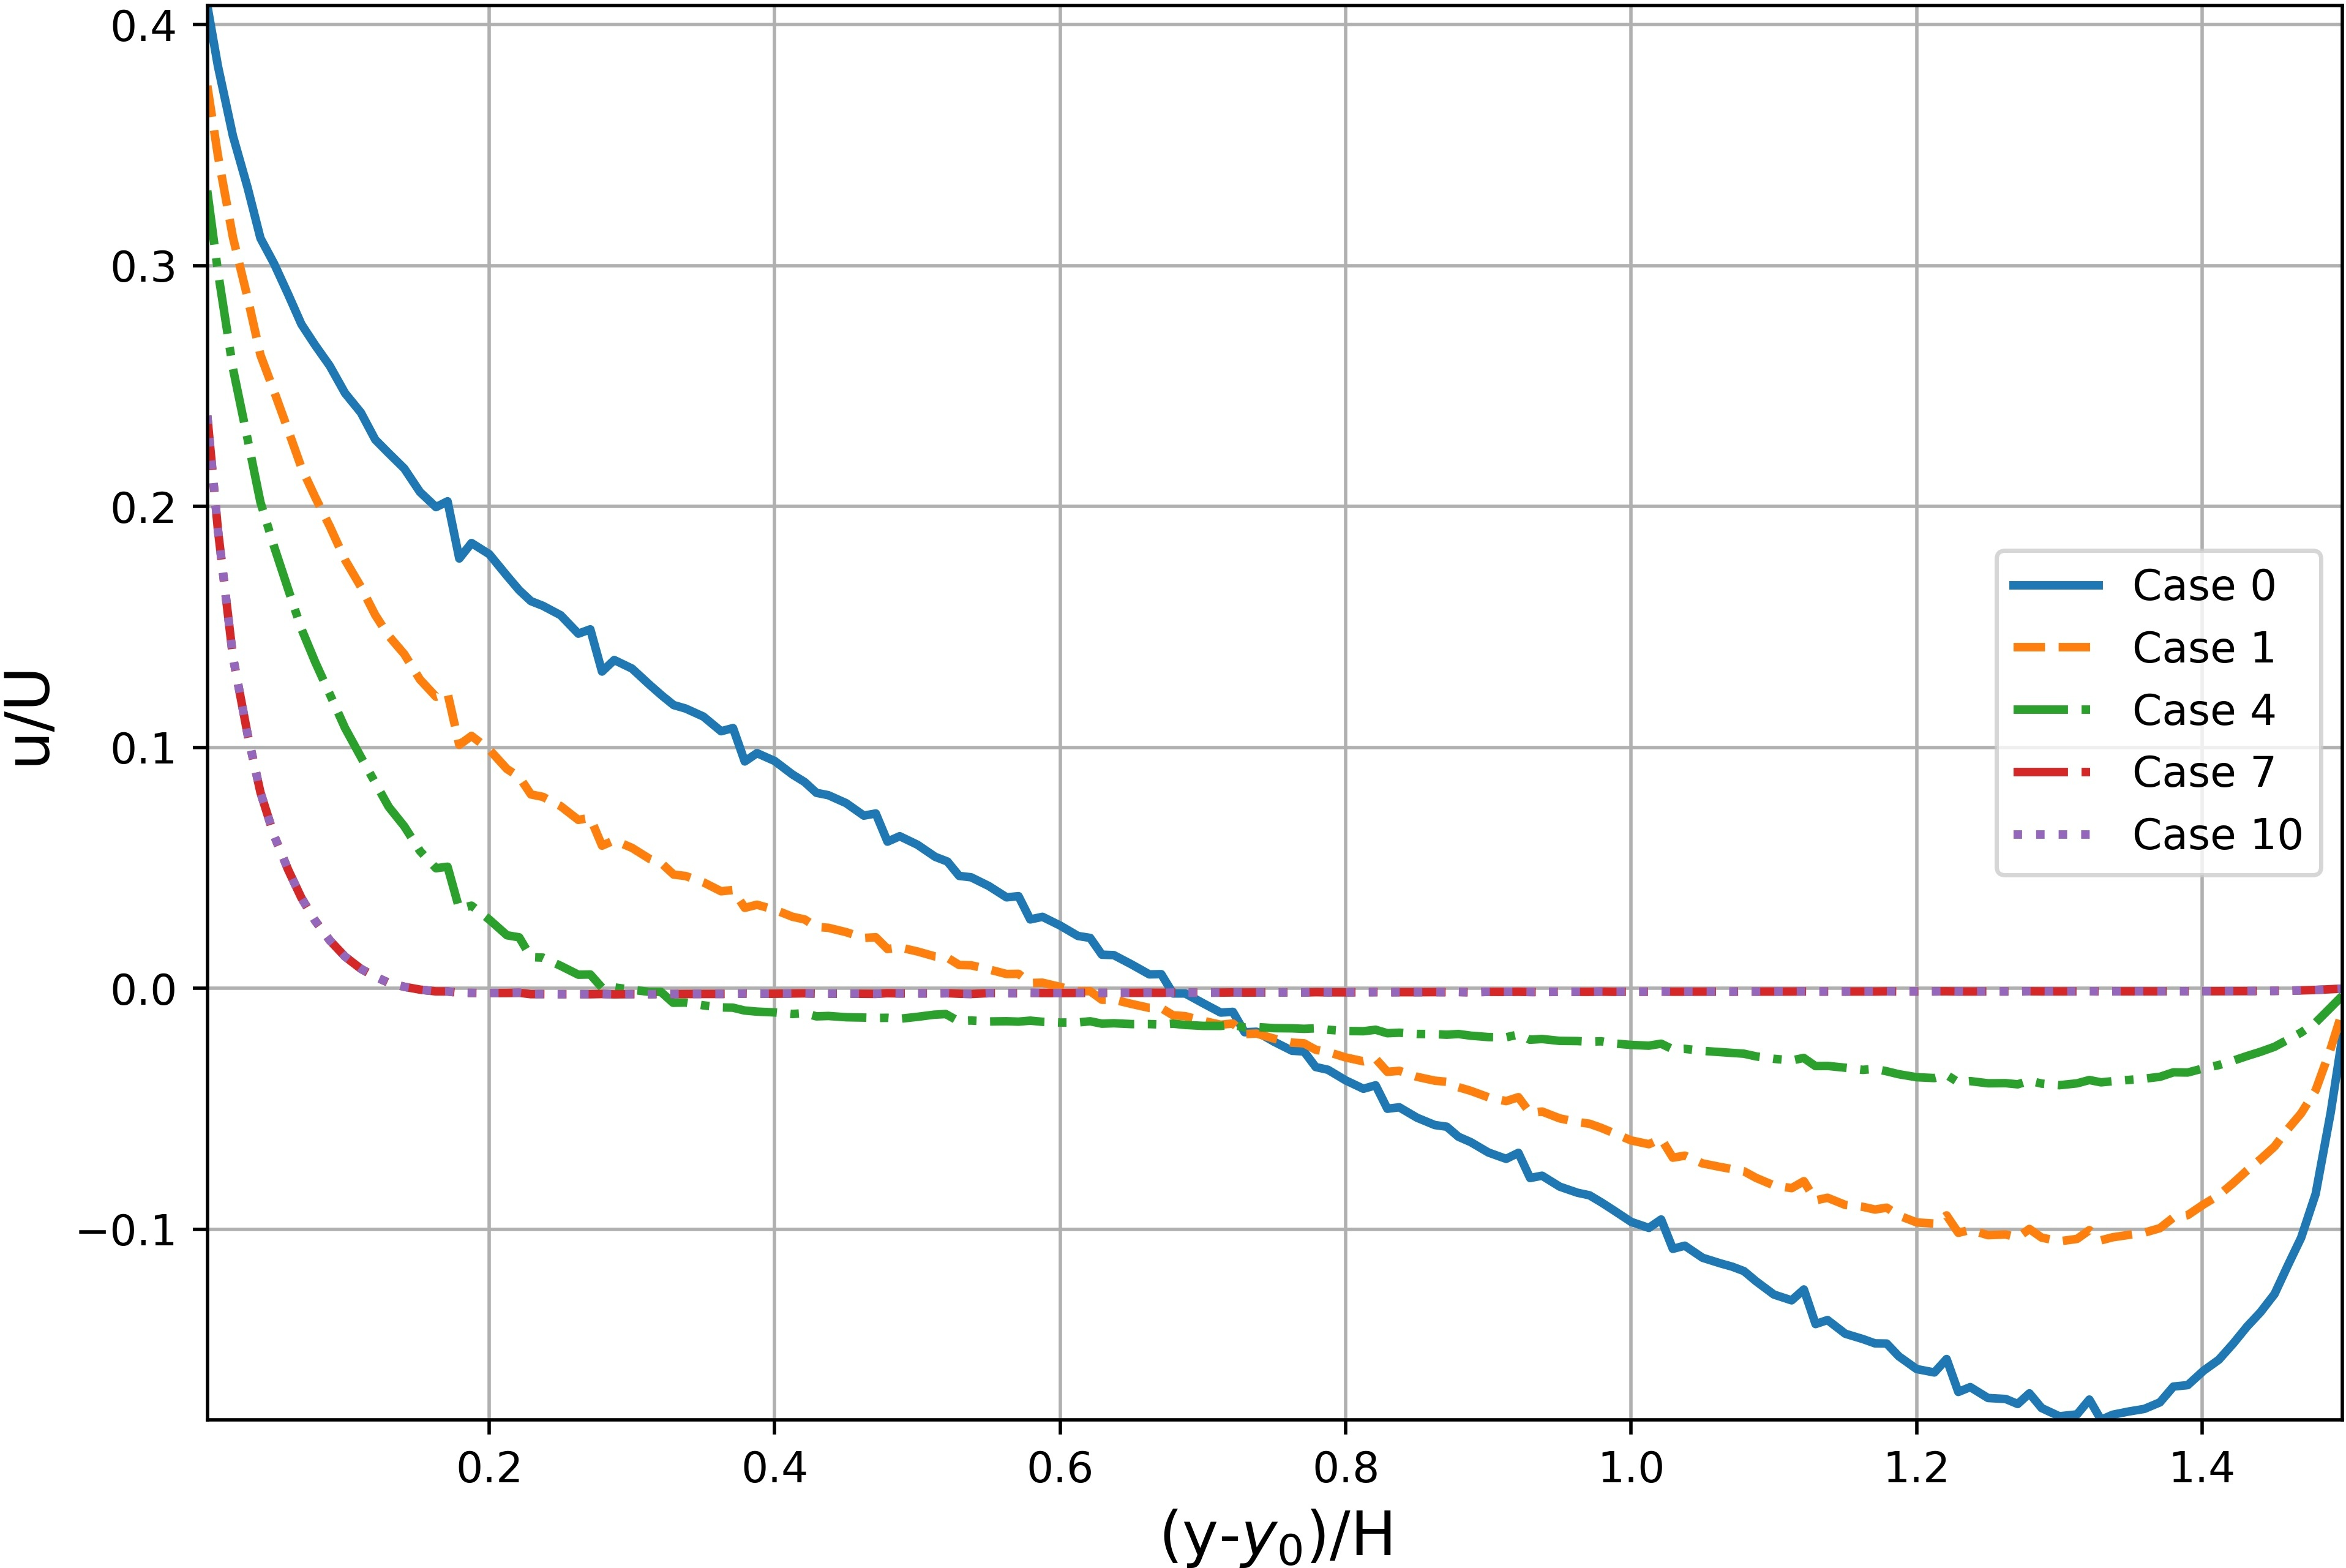
\includegraphics[width=\linewidth]{../images/art4/velXYPlane.jpg}
\caption{The variation of the streamwise velocity at the horizontal plane $z/H = 0.6$.}
\label{fig:art4:velXYPlane}
\end{figure}
The flow through the interface was initially directed toward the cavity ($z/H < 0.1$); positive velocity; then it was outwards ($0.1 < z/H < 0.9$); negative velocity; and lastly entering the domain ($z/H > 0.9$) (Figure \ref{fig:art4:yVelatInterfaceZAxis}). Through the variation in density, this behaviour did not change as the location of the phases did not change through all the cases, as seen in Figure \ref{fig:art4:yVelatInterfaceZAxis}, although the peak velocities at each phase gradually decreased as the vegetation density increased, which is attributable to the energy dissipation caused by vegetation. As the velocity values decreased the second phase ($0.1 < z/H < 0.9$) tended to flat as the vegetation was tending to a solid block behaviour similar to the behaviour of vegetation in \cite{chen2012}. Furthermore, the initial peak in velocity disappeared for $a > 5.32$\% (Case 8) and was substituted by the increase of the third phase.

\begin{figure}[!ht]
\centering
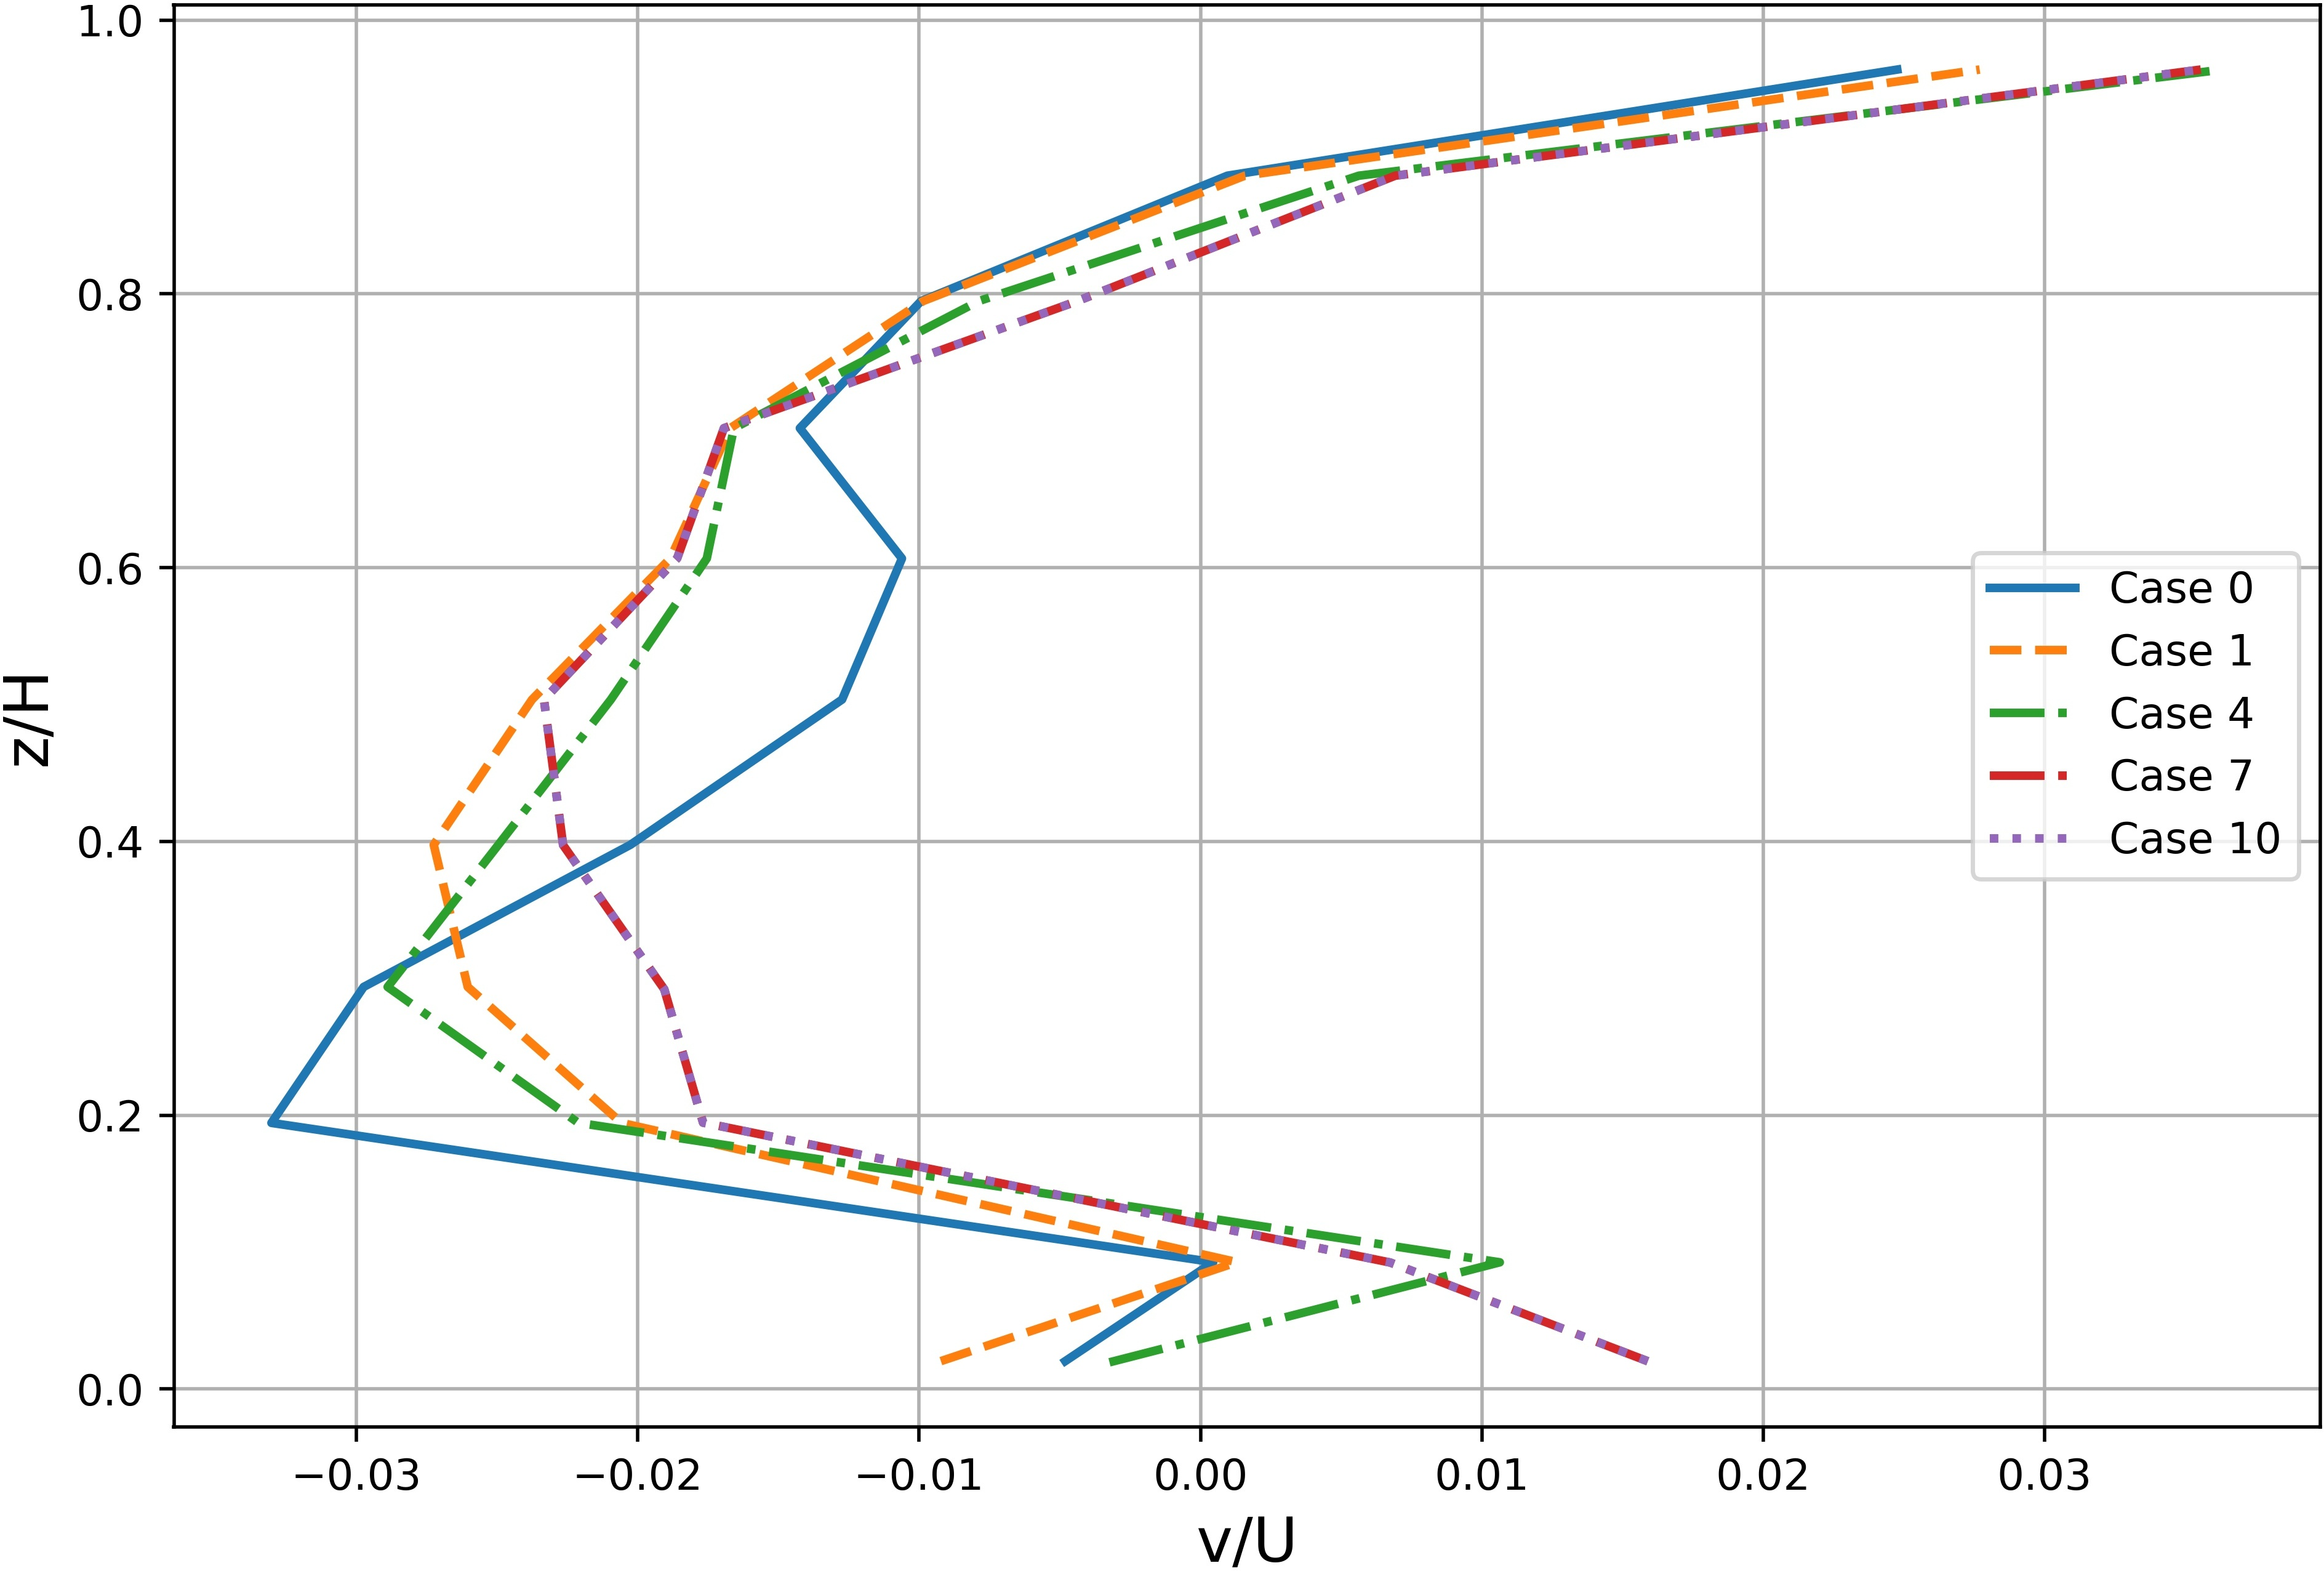
\includegraphics[width=\linewidth]{../images/art4/yVelatInterfaceZAxis.jpg}
\caption{The variation of the transversal velocity in the interface between the cavity and the main channel along the z-axis: a) Cases from 0 to 5; b) Cases from 5 to 10. Positive values of $v/U$ indicate the flow entering the cavity volume.}
\label{fig:art4:yVelatInterfaceZAxis}
\end{figure}

Figure \ref{fig:art4:yVelatInterfaceXAxis} shows the behaviour of the interface along the \textit{x}-axis. Analogous to the \textit{z}-axis, the increase in vegetation density altered the velocity zones. When the vegetation was not present, Case 0, the profile initially was set to the main channel up to 50 \% of the interface length similar to the behaviour of the series of groynes in \textcite{weitbrecht2004}. Although, with the increase of vegetation this first negative zone became positive and the only region where water exited the DZ volume was tending to $(x-x0)/L > 0.8$, due to the shock of the vortices to the downstream wall of the cavity.

\begin{figure}[!ht]
\centering
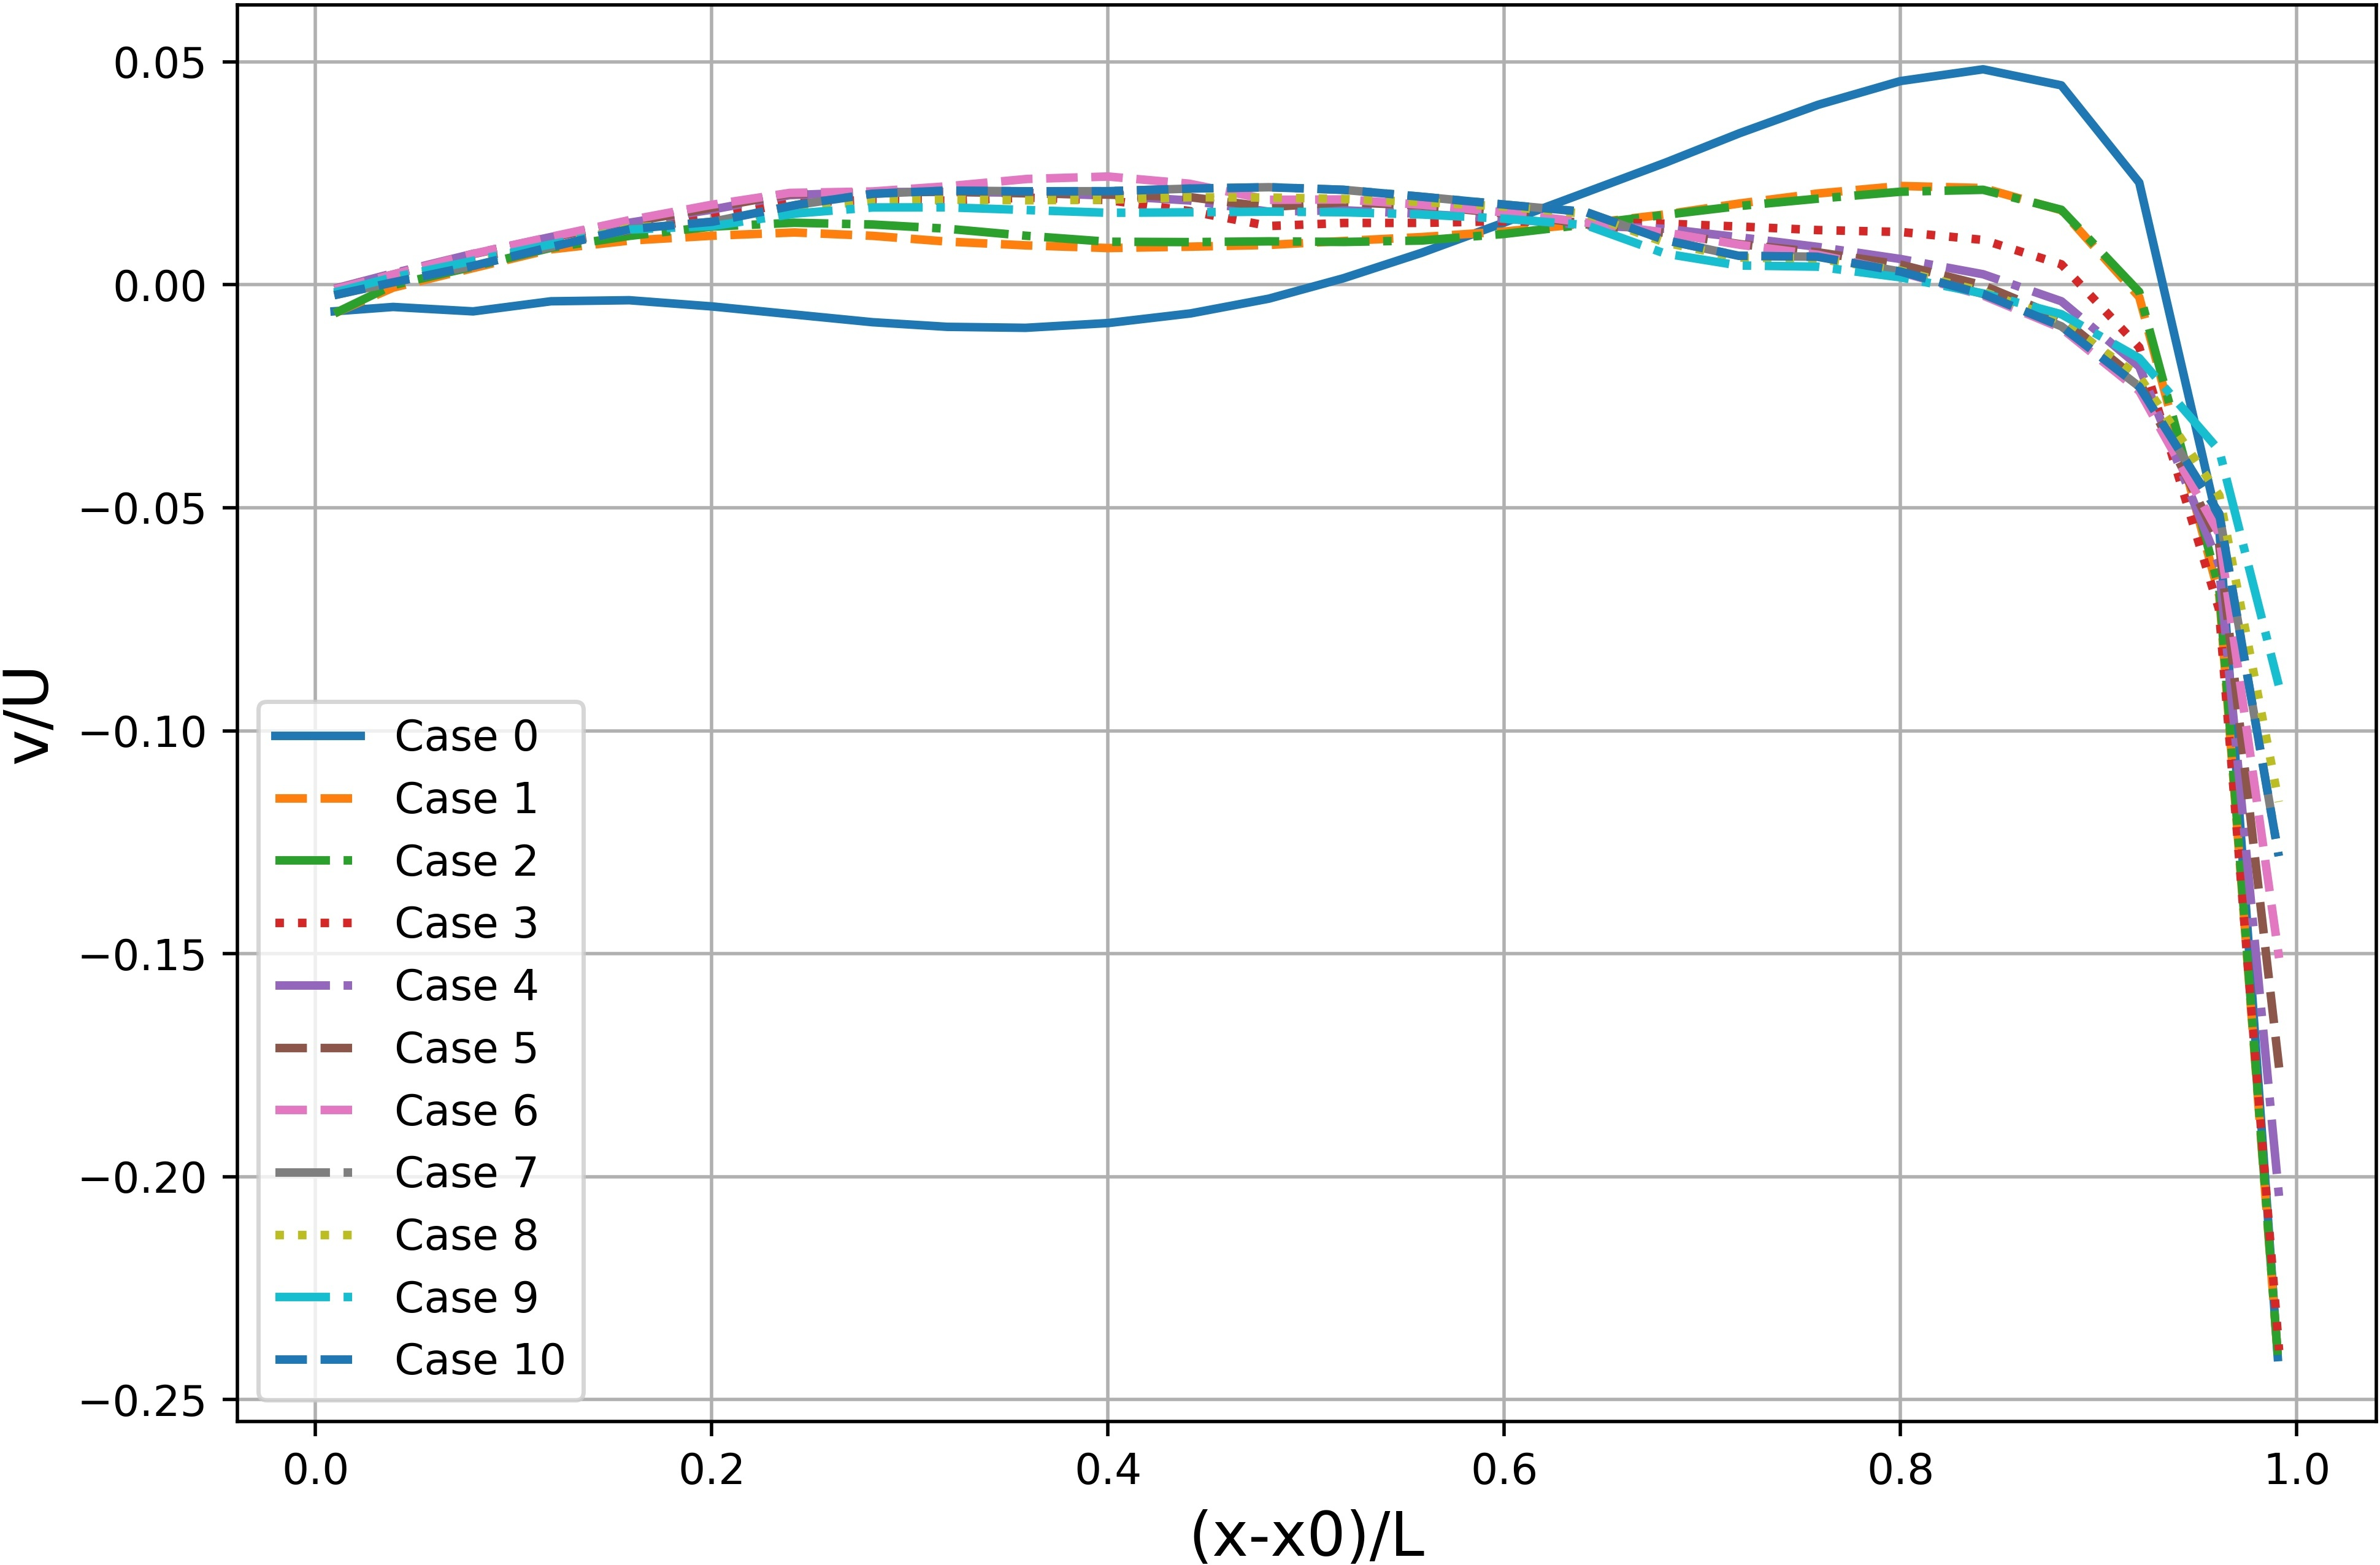
\includegraphics[width=\linewidth]{../images/art4/yVelatInterfaceXAxis.jpg}
\caption{The variation of the transversal velocity in the interface between the cavity and the main channel along the x-axis. Positive values of $v/U$ indicate the flow entering the cavity volume.}
\label{fig:art4:yVelatInterfaceXAxis}
\end{figure}

\section{Hydrodynamics of the Mixing Layer}
\subsection{Thickness of the Mixing Layer}
The mixing layer is a region that is developed along the interface due to a velocity gap between the lateral cavity and the main channel. The adoption of a thickness $\delta$  (m) of the mixing layer is commonly used to describe the spreading angle of the mixing layer and the range of velocity gradients between the zones \cite{xiang2020,Mignot2017,Yossef2011}. \textcite{xiang2020} suggested that the thickness could be divided into an inner section $\delta_{in}$  (m) (in the cavity) and an outer section $\delta_{out}$  (m) (in the main channel). The total thickness  is defined as:
\begin{equation}
\delta=\delta_{in}+\delta_{out}=\frac{U_i(x)-U_c(x)}{\left (\partial \bar{u} / \partial y  \right )_{max}}+\frac{U_m(x)+U_i(x)}{\left (\partial \bar{u} / \partial y  \right )_{max}}
\label{eqn:art4:thickness}
\end{equation}

where, $U_i$, $U_c$ and $U_m$ (m/s) are the time-averaged streamwise velocities at the interface, in the cavity and the main channel. These velocities were extracted where the velocity gradient is negligibly small, i.e., lower than 0.5 $s^{-1}$ in reference to \textcite{xiang2020,Mignot2017}. $\left (\partial \bar{u} / \partial y  \right )_{max}$ represents the maximum velocity gradient at each x position along the interface.

Figure \ref{fig:art4:thickness} show the evolution of the thickness layer in the streamwise direction for all the cases. Overall, the mixing layer increased when $(x-x_0)/L<0.80$ and decreased when $(x-x_0)/L>0.80$ as the velocity gradient increased in the contact with the wall. Similar to \textcite{xiang2020}, the vegetation density increase affected the width of the mixing layer, for both inner and outer sections. The increasing blockage limited the entrance of flow in the cavity (Figures \ref{fig:art4:velocityContour} and \ref{fig:art4:velXYPlane}), thus it limits the growth of the mixing layer. The wall behaviour of the cavity started to take place in case 8 and 9, although the presence of the secondary gyre in case 10 increased the thickness.

\begin{figure}[!ht]
\centering
\includegraphics[width=\linewidth]{../images/art4/thickness.jpeg}
\caption{Evolution of the mixing layer thickness averaged at the z-axis: a) inner mixing layer; b) outer mixing layer and c) total mixing layer.}
\label{fig:art4:thickness}
\end{figure}

\subsection{Vorticity}
Figures \ref{fig:art4:vorticityMean1} and \ref{fig:art4:vorticityMean2} show the time-averaged vorticity magnitude (normalised by U/H) at . The vorticity magnitude $\Omega$ ($s^{-1}$) is defined as:

\begin{equation}
\Omega = \nabla \times \vec{v}
\label{eqn:art4:vorticity}
\end{equation}

where, $\vec{v}$ (m/s) is the velocity vector.

For all cases, the vorticity remained high through all the interface between the cavity and the main channel. The maximum vorticity occurred at the upstream of the interface ($x/L<0.3$) and decreases in the downstream direction ($x/L>0.3$). Similar to groynes, this effect occurs to the shredding of vortex from the beginning of the cavity \textcite{xiang2020}. As the eddies shred, the high vorticity region increases in width (\textit{y}-axis) to its maximum value at the downstream wall. This width reduces as the vegetation density increases due to higher drag.

The increase of vegetation density gradually decreased the levels of vorticity inside the cavity volume up to $a<7.9920$, when there was no more vorticity in the volume. Although, it seems that vegetation increased the vorticity at the inner part of the mixing layer despite the blockage effect.

\begin{figure}[!ht]
\centering
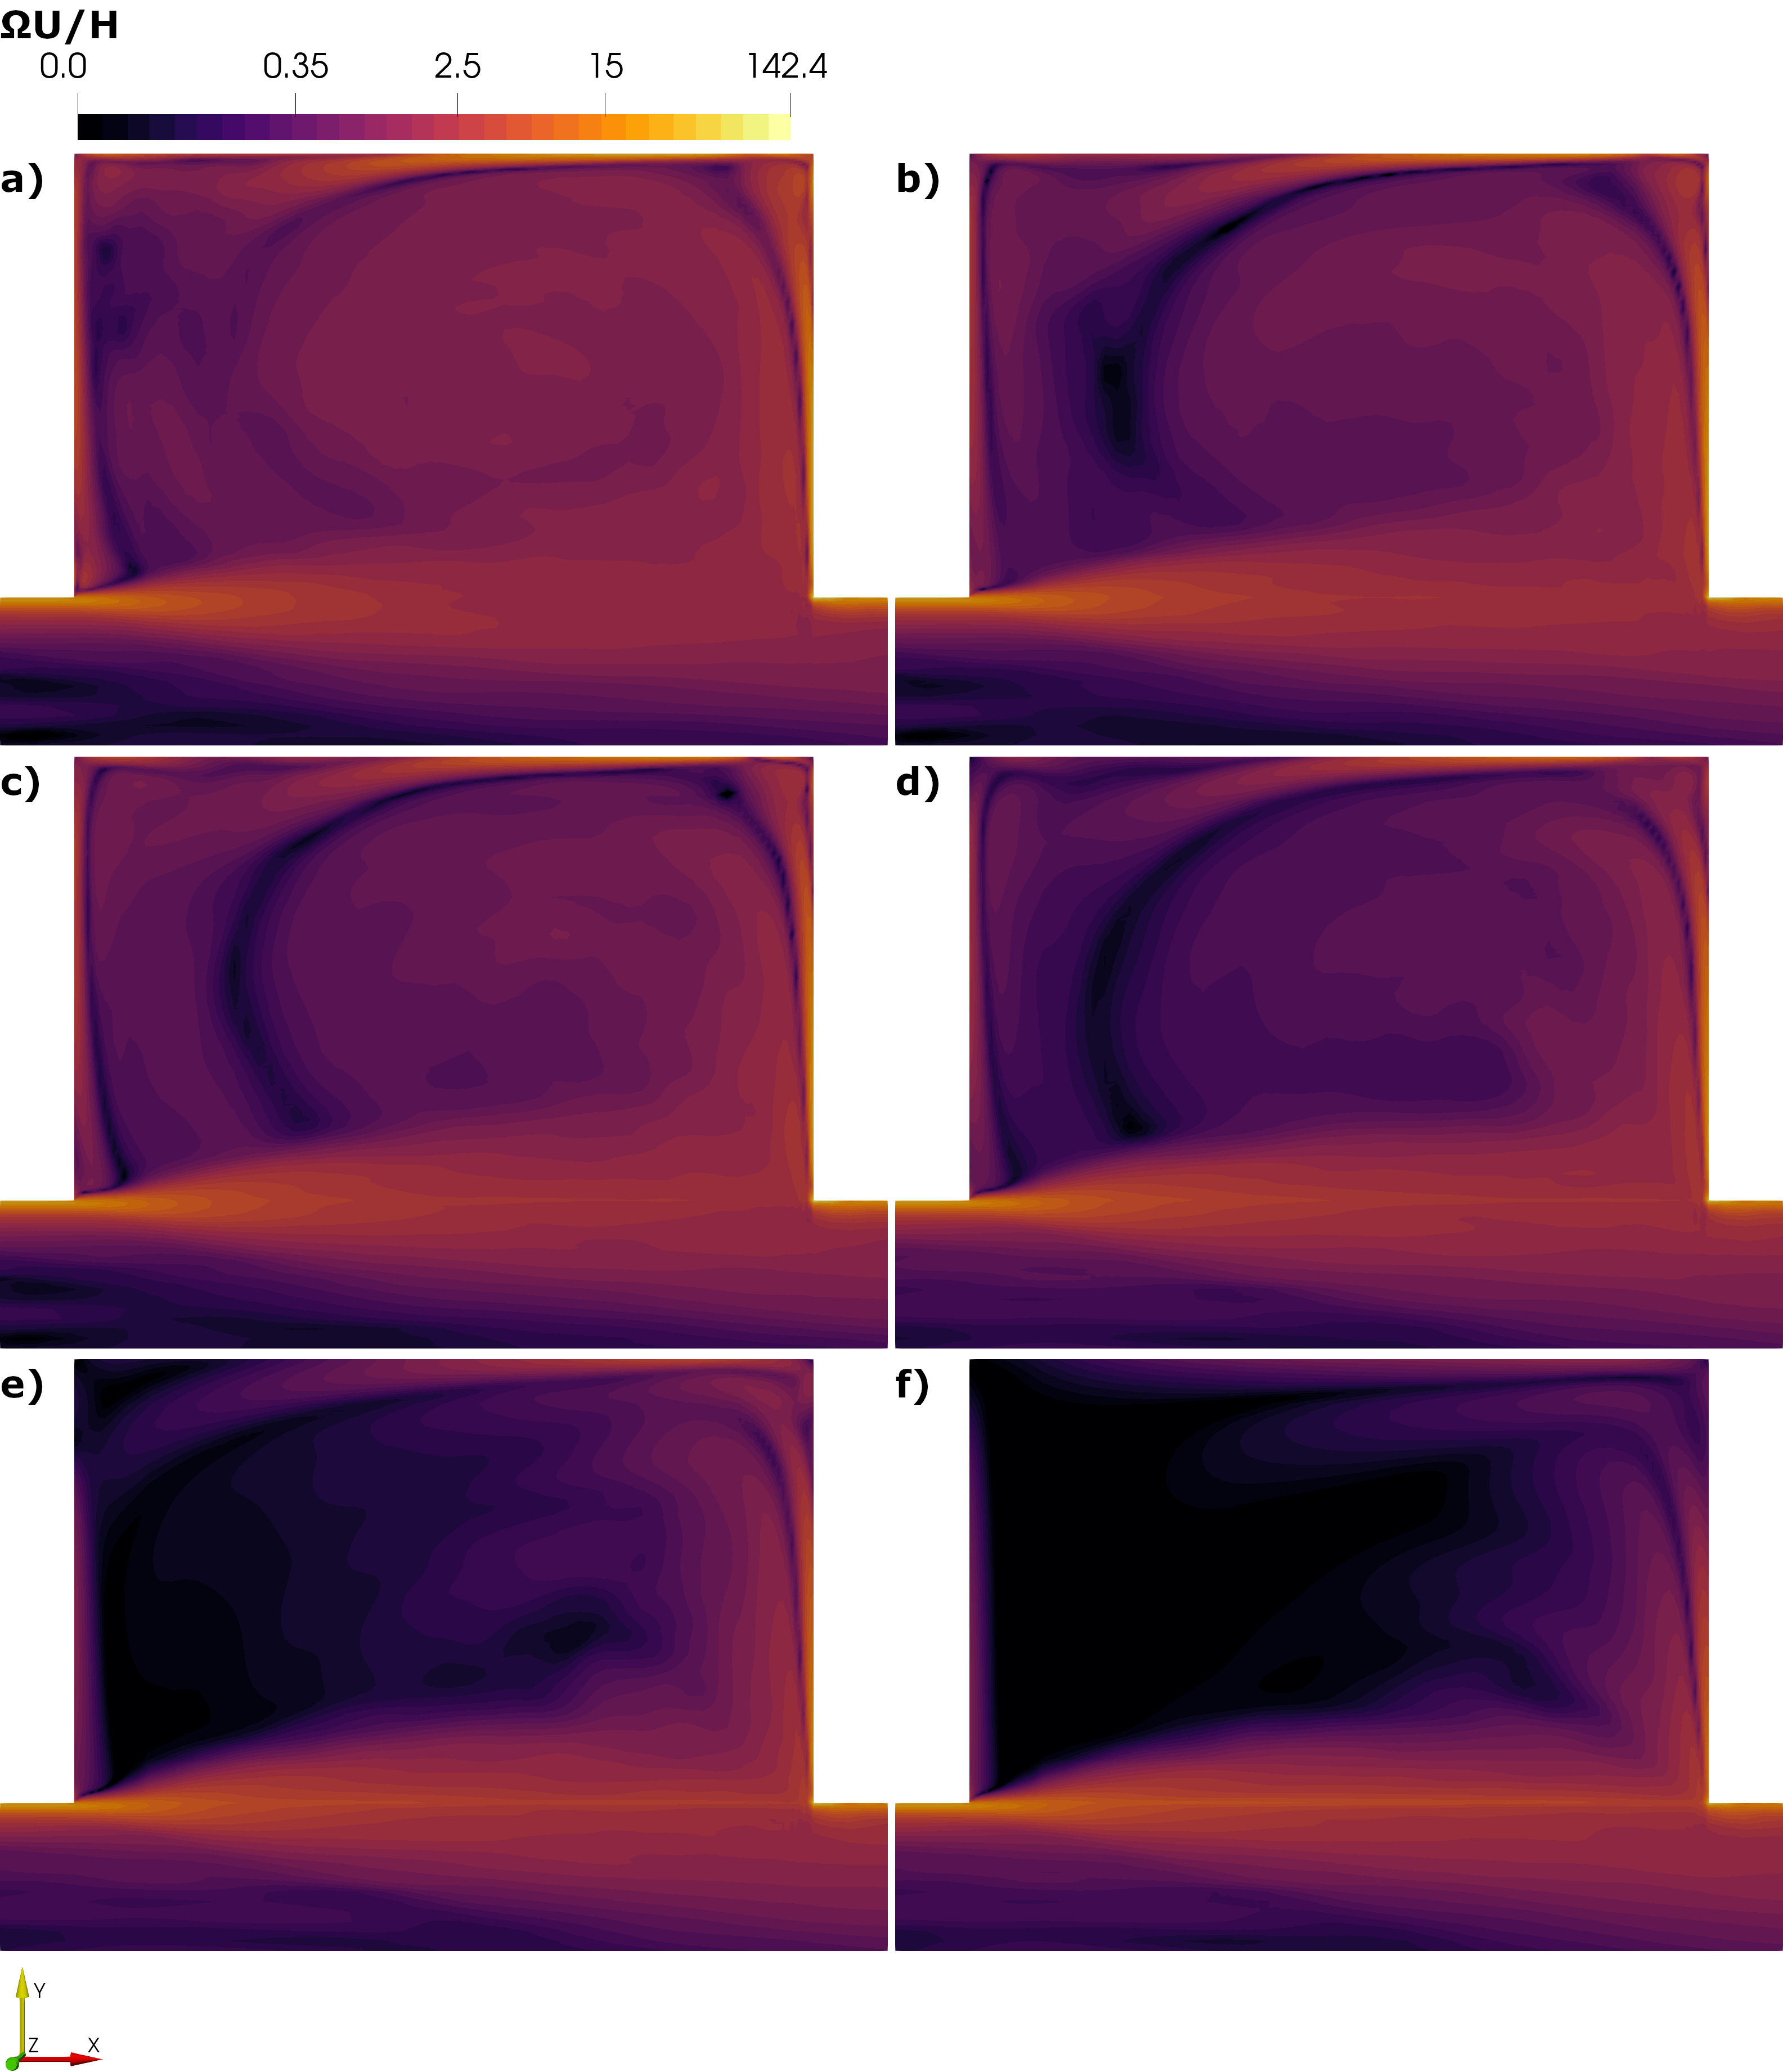
\includegraphics[width=\linewidth]{../images/art4/vorticityMean1.jpeg}
\caption{Time averaged vorticity at z/H = 0.6: a) Case 0, b) Case 1, c) Case 2, d) Case 3, e) Case 4 and f) Case 5.}
\label{fig:art4:vorticityMean1}
\end{figure}

\begin{figure}[!ht]
\centering
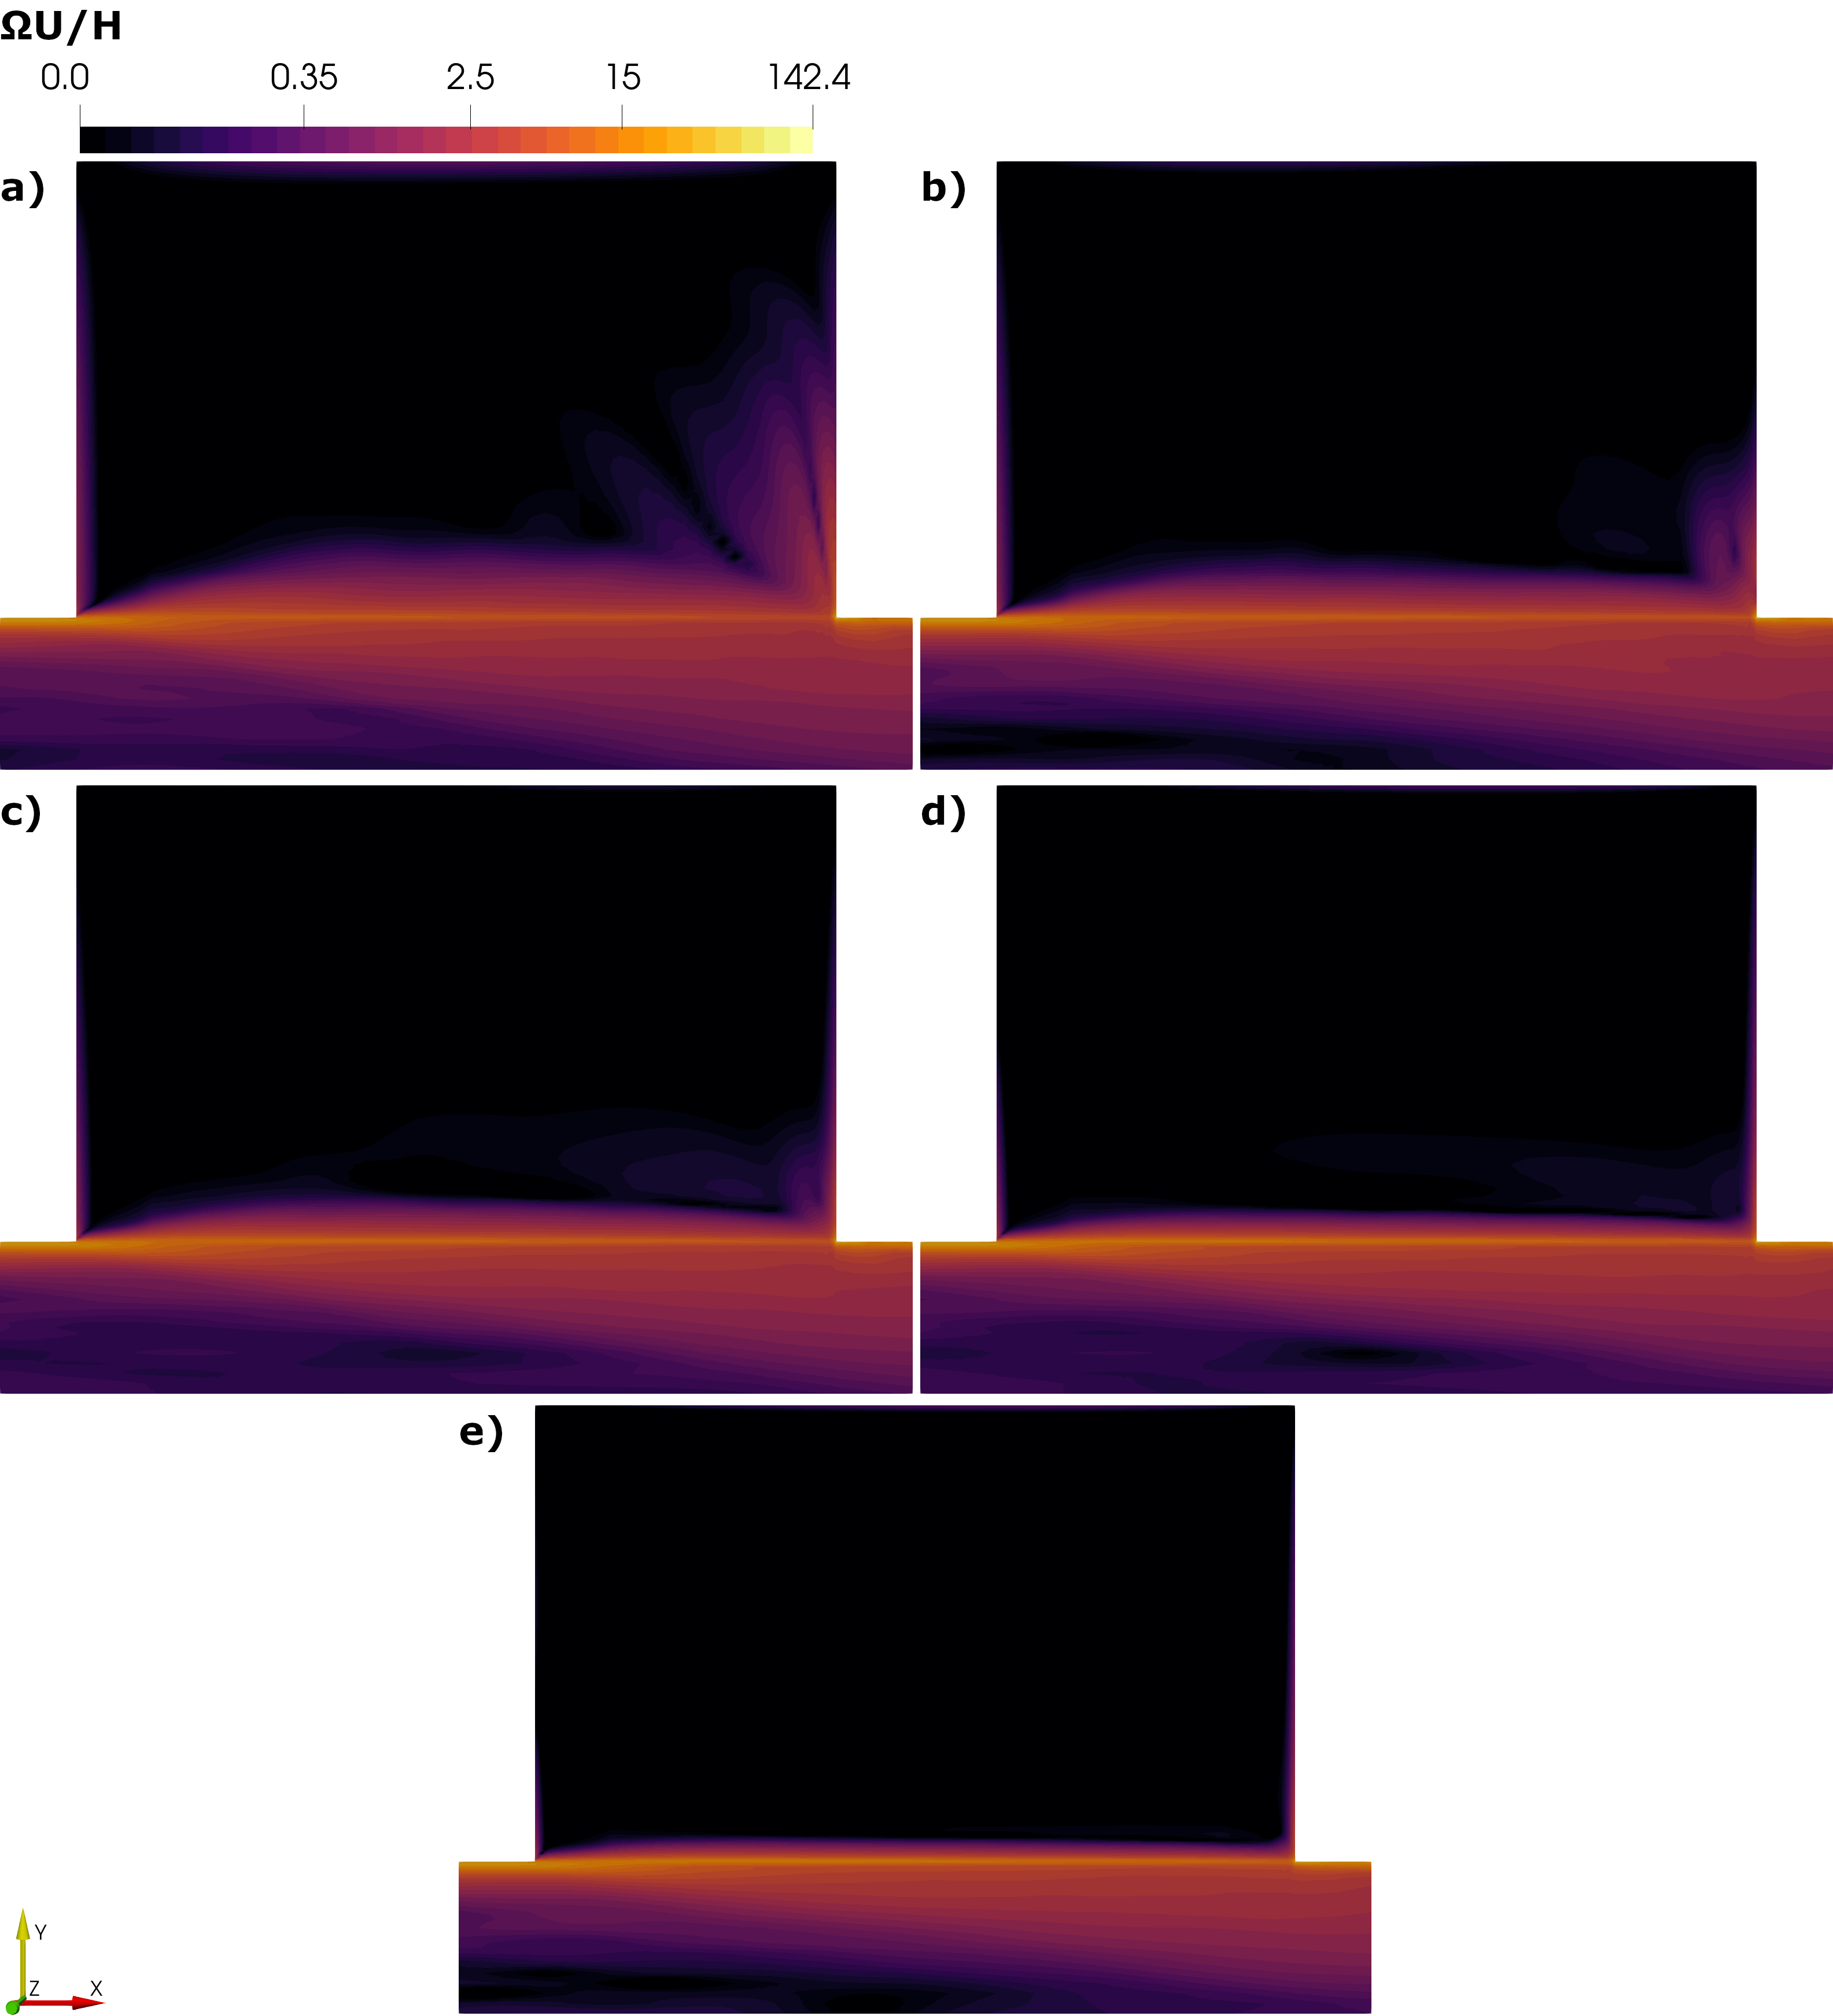
\includegraphics[width=\linewidth]{../images/art4/vorticityMean2.jpeg}
\caption{Time averaged vorticity at z/H = 0.6: a) Case 6, b) Case 7, c) Case 8, d) Case 9 and e) Case 10.}
\label{fig:art4:vorticityMean2}
\end{figure}

\subsection{Turbulent Kinetic Energy (TKE)}
The turbulent kinetic energy (TKE) in a LES simulation is defined as:
\begin{equation}
TKE = 0.5 tr(R) + 0.5 tr(u')
\label{eqn:art4:tke}
\end{equation}

where, $R$ (m2/s2) is the Reynolds stress tensor and $u’$ (m/s) is the instantaneous fluctuation tensor.

A time-averaged TKE distribution, normalised by $U^2$, is presented in Figures \ref{fig:art4:totalTKEMean1} and \ref{fig:art4:totalTKEMean2}. Through all interface, the values of TKE remained above $TKE/U^2 > 0.05$, at the downstream of the interface the maximum value occurred. At this same region, the vortex encounters the cavity lateral wall, the portion that enters the cavity reduces in magnitude as it moves through the vegetation. In an unvegetated scenario Figure \ref{fig:art4:totalTKEMean1} a) the TKE followed all the main circulation, behaviour that did not occur with the presence of vegetation. Hence the increase in vegetation density reduced the values of TKE, analogously to the vorticity.

As the vegetation density increased, the turbulent kinetic energy inside the cavity decreased, similarly to \textcite{xiang2019}, although in a much faster rate than the vorticity. The blockage effect due to the vegetation density increase slowly reduces the TKE values inside the cavity. The last region in which $TKE > 0$ is the downstream wall of the cavity, region where the first jet enters the volume. Similar to \textcite{xiang2019}, the first levels of vegetation registered an increase of TKE at the interface. Although with the increase of vegetation beyond $a > 0.33$\% (Figure \ref{fig:art4:totalTKEMean1} d), the turbulence intensity was lower than the non vegetated scenario which can be attributed to the shrink of the inner part of the mixing layer (Figure \ref{fig:art4:thickness} a) caused by the flow turbulence inhibition caused by high-density vegetation \cite{Nepf2012}. Furthermore, the shape of the TKE distribution on the outer part of the mixing layer changed with the increase of vegetation, on $a = 0$\% the region that the distribution width increases is up to approximately $(x-x0)/L < 0.8$, when the jet entrance to the volume decreases its width. For the vegetated cases, specially Case 3, the vegetation blocks part of the jet that normally enters the downstream portion of the volume, this causes the TKE distribution to take a triangular shape which indicates an increased turbulence intensity in the main channel up to $a < 5.328$ \%.

\begin{figure}[!ht]
\centering
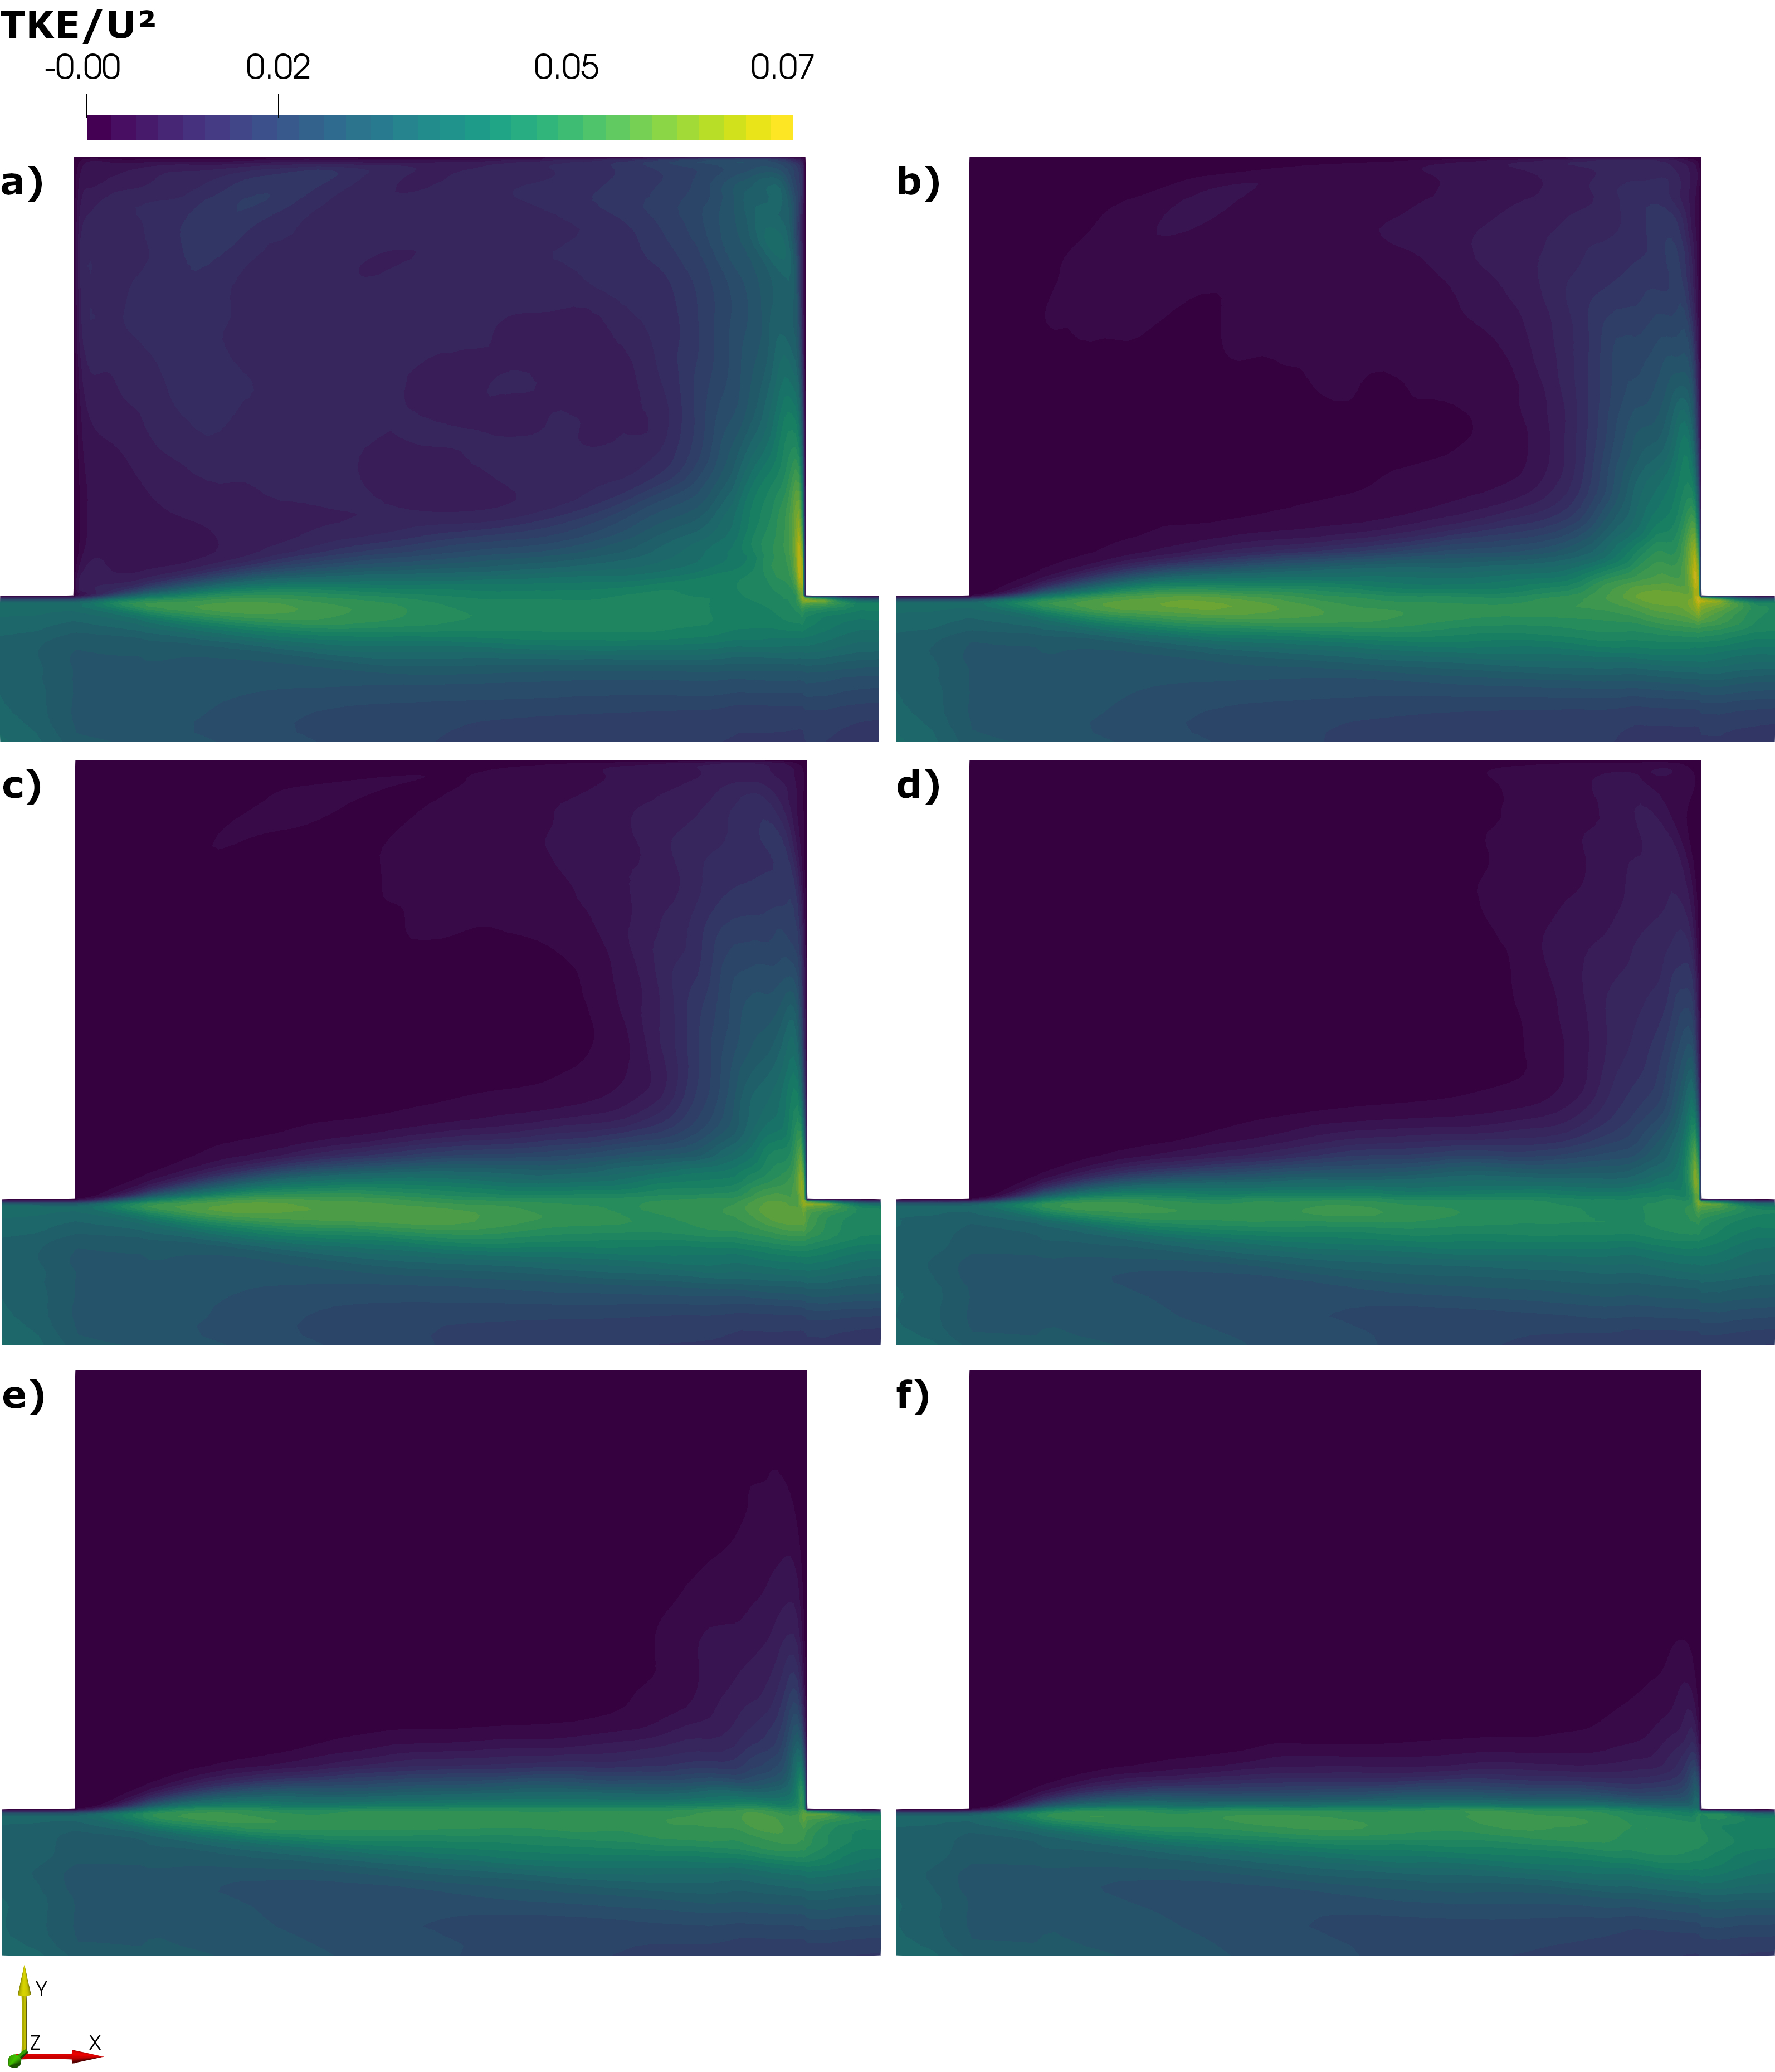
\includegraphics[width=\linewidth]{../images/art4/totalTKEMean1.jpeg}
\caption{Time-averaged total kinetic energy (TKE) at z/h = 0.6: a) Case 0, b) Case 1, c) Case 2, d) Case 3, e) Case 4 and f) Case 5.}
\label{fig:art4:totalTKEMean1}
\end{figure}

\begin{figure}[!ht]
\centering
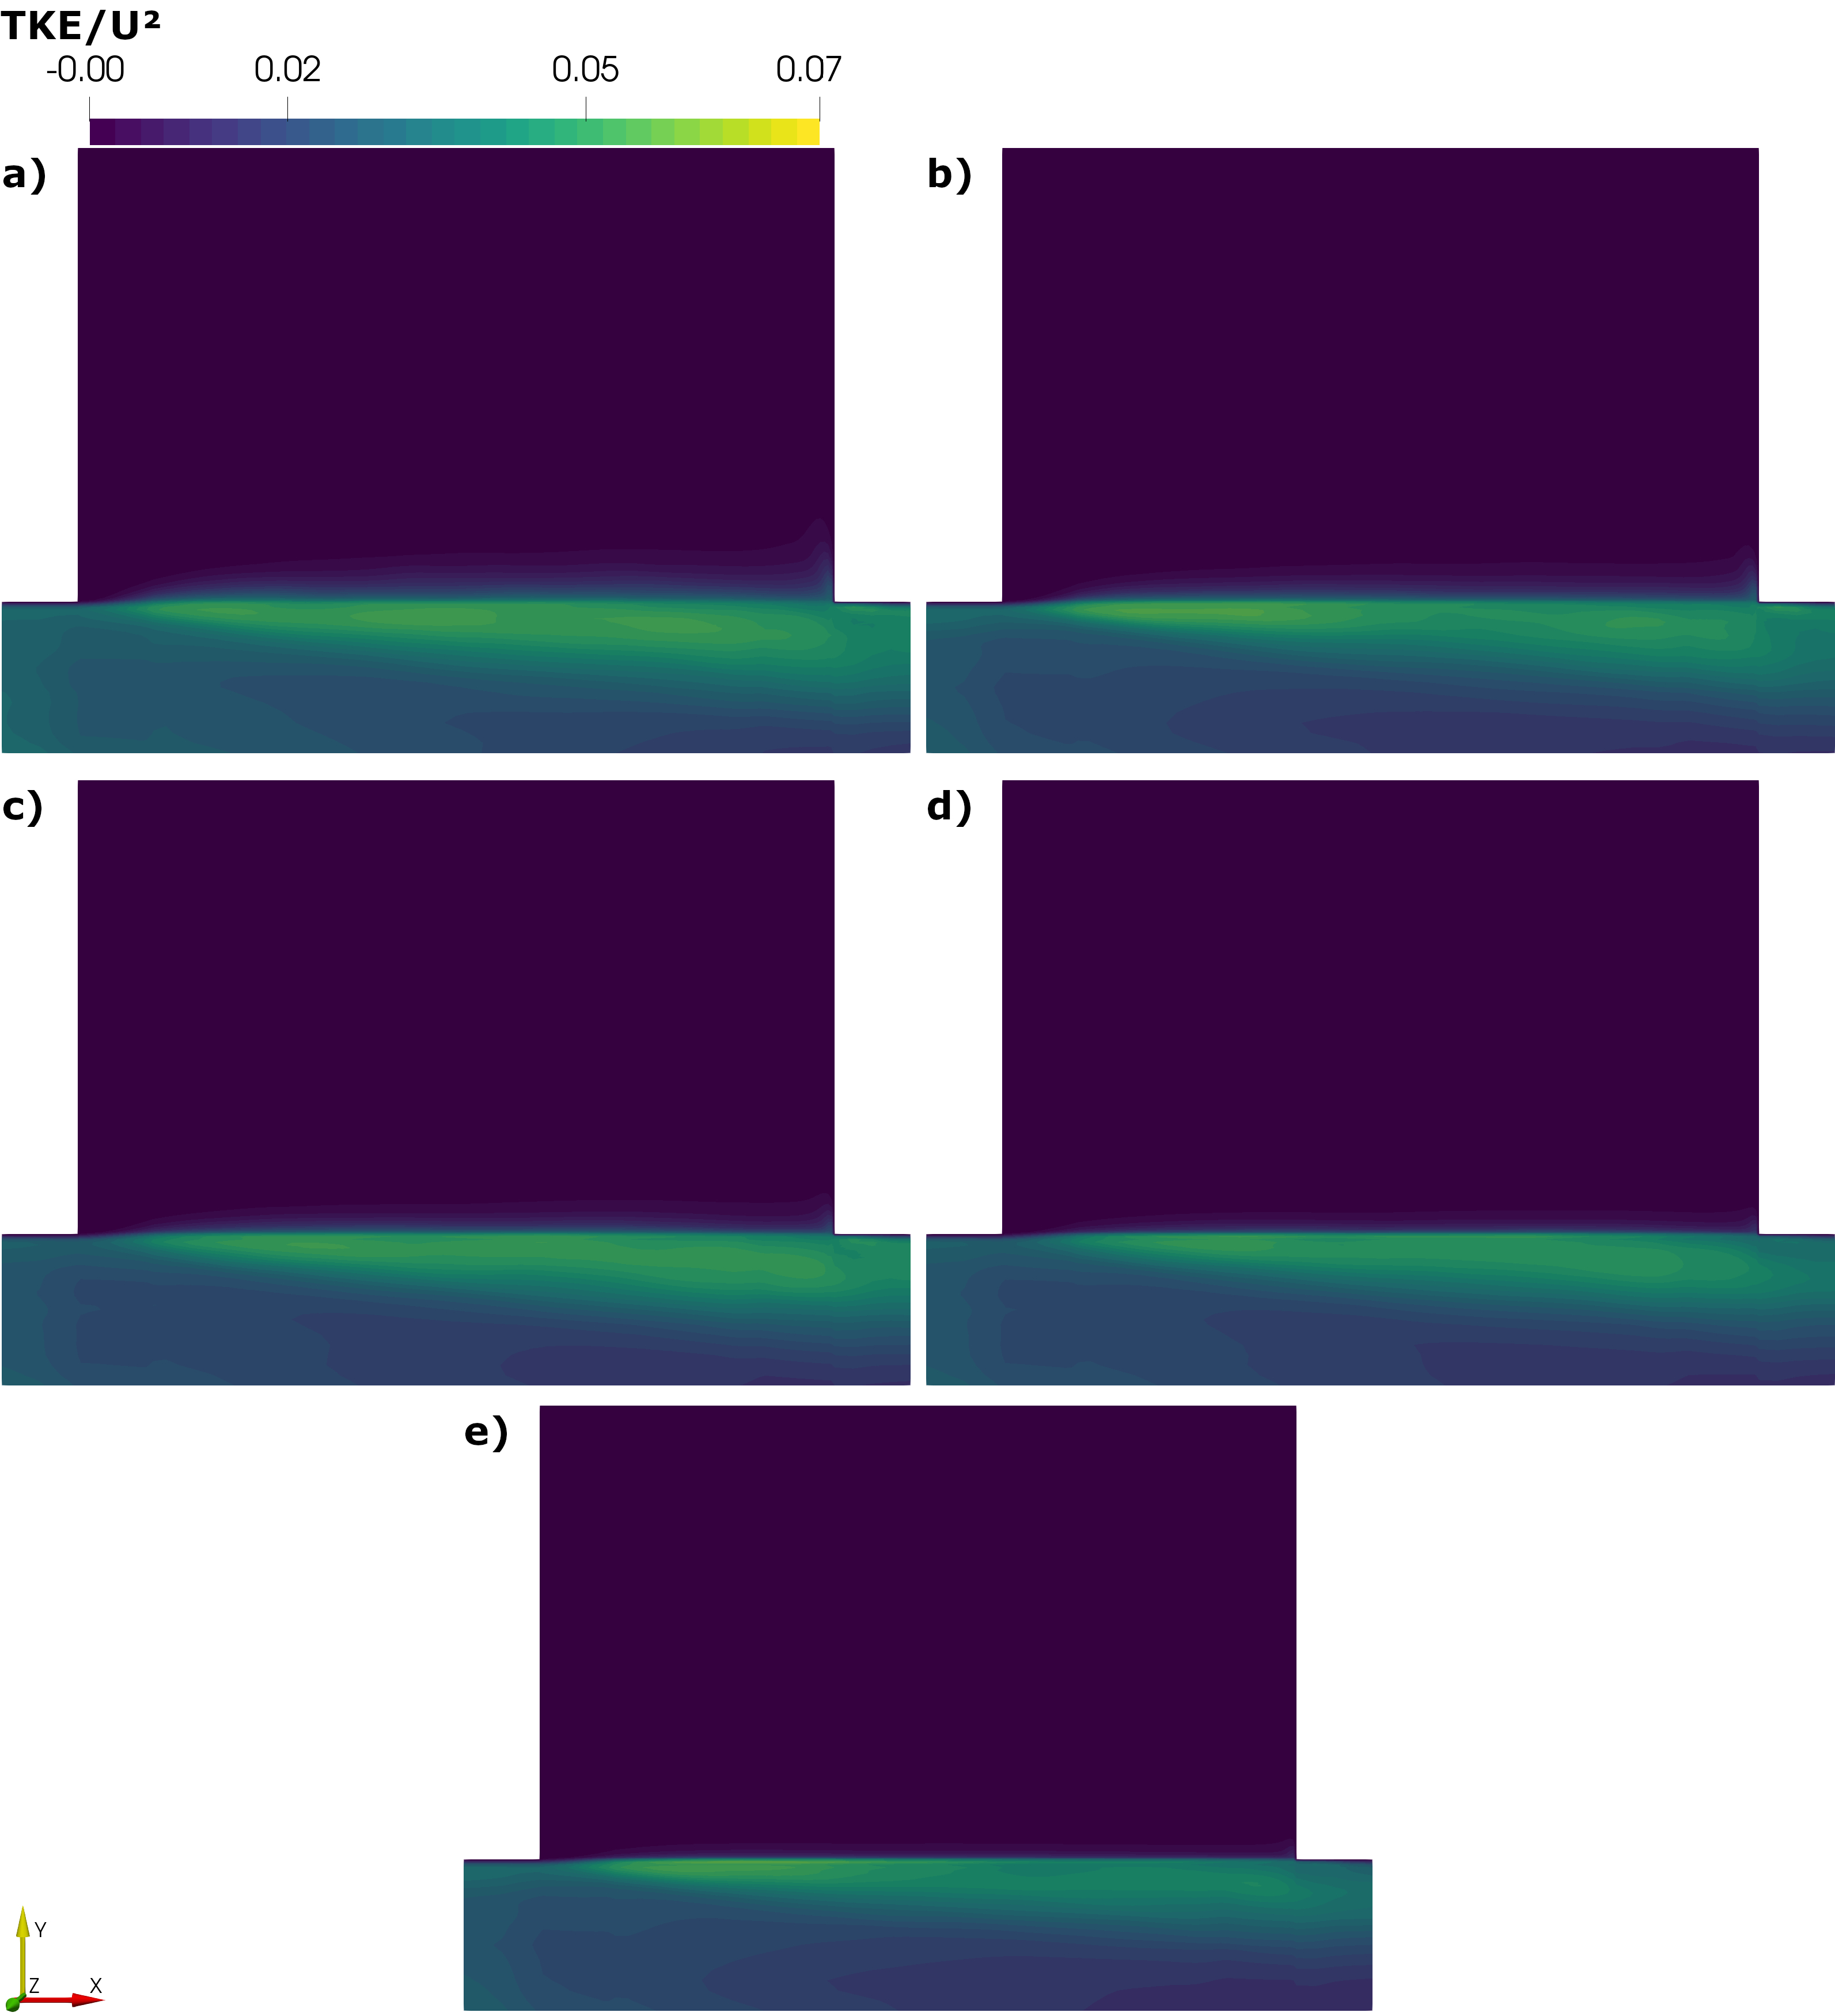
\includegraphics[width=\linewidth]{../images/art4/totalTKEMean2.jpeg}
\caption{Time-averaged total kinetic energy (TKE) at z/h = 0.6: a) Case 6, b) Case 7, c) Case 8, d) Case 9 and e) Case 10.}
\label{fig:art4:totalTKEMean2}
\end{figure}

\section{Mass Exchange}
The mass exchange coefficient $k$ is an important parameter of the cavity, as one of its main characteristics is the transient storage of mass. This coefficient indicates the mass exchange rate between the cavity and the main channel. The evaluation of this parameter through tracer experiments was done using a first-order exponential decay in which the initial concentration was set to 1. Analogously, the mean retention time ($T_{cav}$) is the time needed to completely replace the water volume in the cavity. This parameter was adjusted using a non-linear least square method to best approximate the value of $T_{cav}$ to the volumetric-average tracer concentration through time \cite{weitbrecht2004} (Figure \ref{fig:art4:massConcentration}).

\begin{equation}
C=C_0 e^{-t/T_{cav}}
\label{eqn:art4:concentration}
\end{equation}

\begin{equation}
k=\frac{W}{T_{cav} U}
\label{eqn:art4:k}
\end{equation}

where, $C_0=1$ is the initial concentration, $t$ (s) is the time and $T_{cav}$ (s) is the mean retention time and $k$ is the mass exchange coefficient.

\begin{figure}[!ht]
\centering
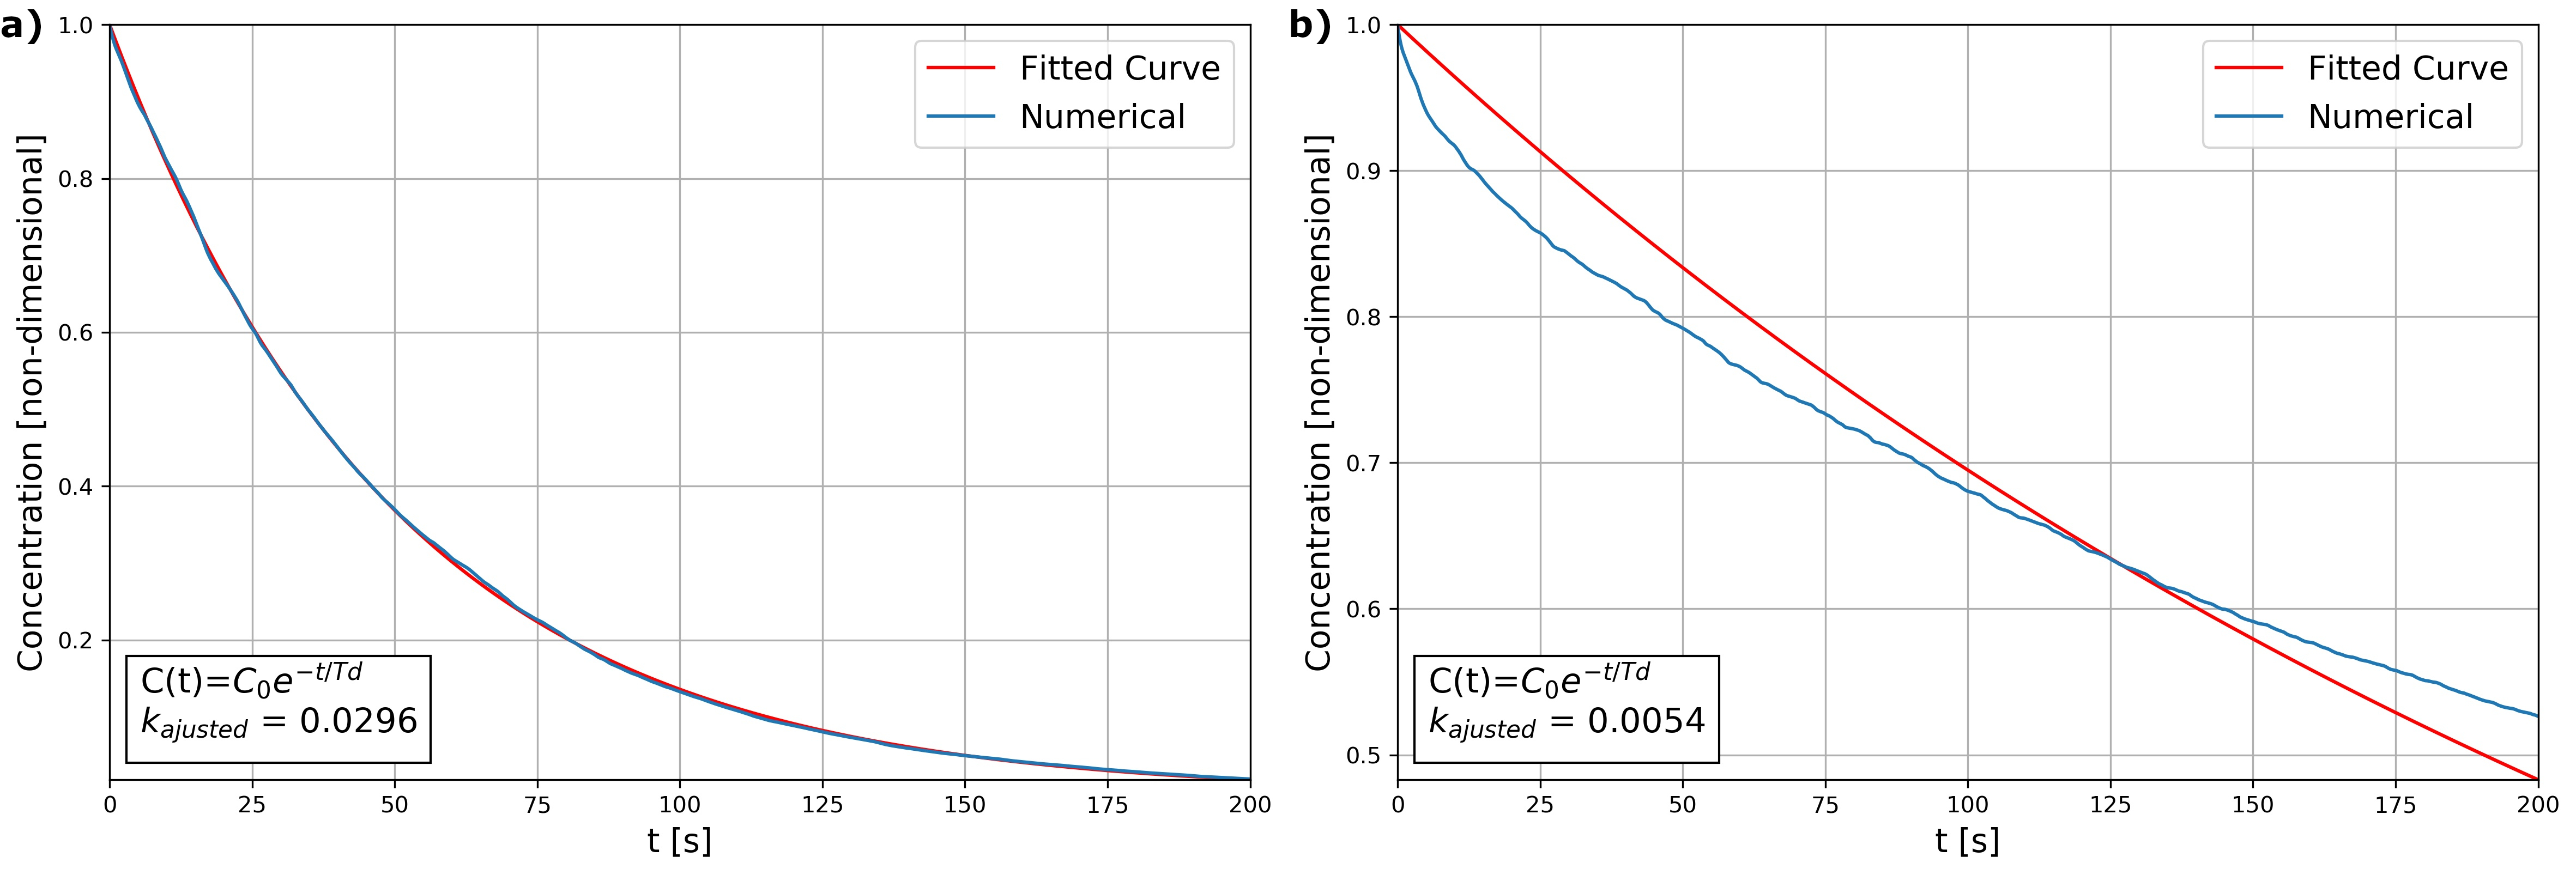
\includegraphics[width=\linewidth]{../images/art4/massDecay.jpeg}
\caption{Volumetric-averaged tracer concentration decay inside the lateral cavity over time: a) Case 1 b) Case 8.}
\label{fig:art4:massConcentration}
\end{figure}

Figure \ref{fig:art4:massExchange} shows the variation of the mass exchange coefficient and the mean retention time with the increase of vegetation density $a$. Analogous to \textcite{xiang2019}, the tracer fields indicated a deviation in the curve near $a \approx 0.33$ which is related first to the plant-induced Karman vortex street and Kelvin-Helmholtz eddies \cite{Nepf2012} which decreased the $k$ decay rate and second the vegetation blockage that becomes the main effect further that point. Further that point, the mass exchange coefficient decreases with the increase of vegetation density in two different phases divided at $a \approx 4$\%. It is possible to assume that this vegetation density acted as a wall as the flow cannot penetrate the cavity enough for the flow to occur, the remaining exchange occurred in a thin layer that further reduced its width as the density increased. The presence of the secondary circulation for $a \geq 5.3280$\% (Case 8) implied that a further increase in vegetation density could divide the secondary phase into a two slope section of the curve, where the first circulation ejects mass faster than the secondary with slower velocities and no contact with the main channel \cite{deOliveira2020} (Figure \ref{fig:art4:massConcentration} a and b).

\begin{figure}[!ht]
\centering
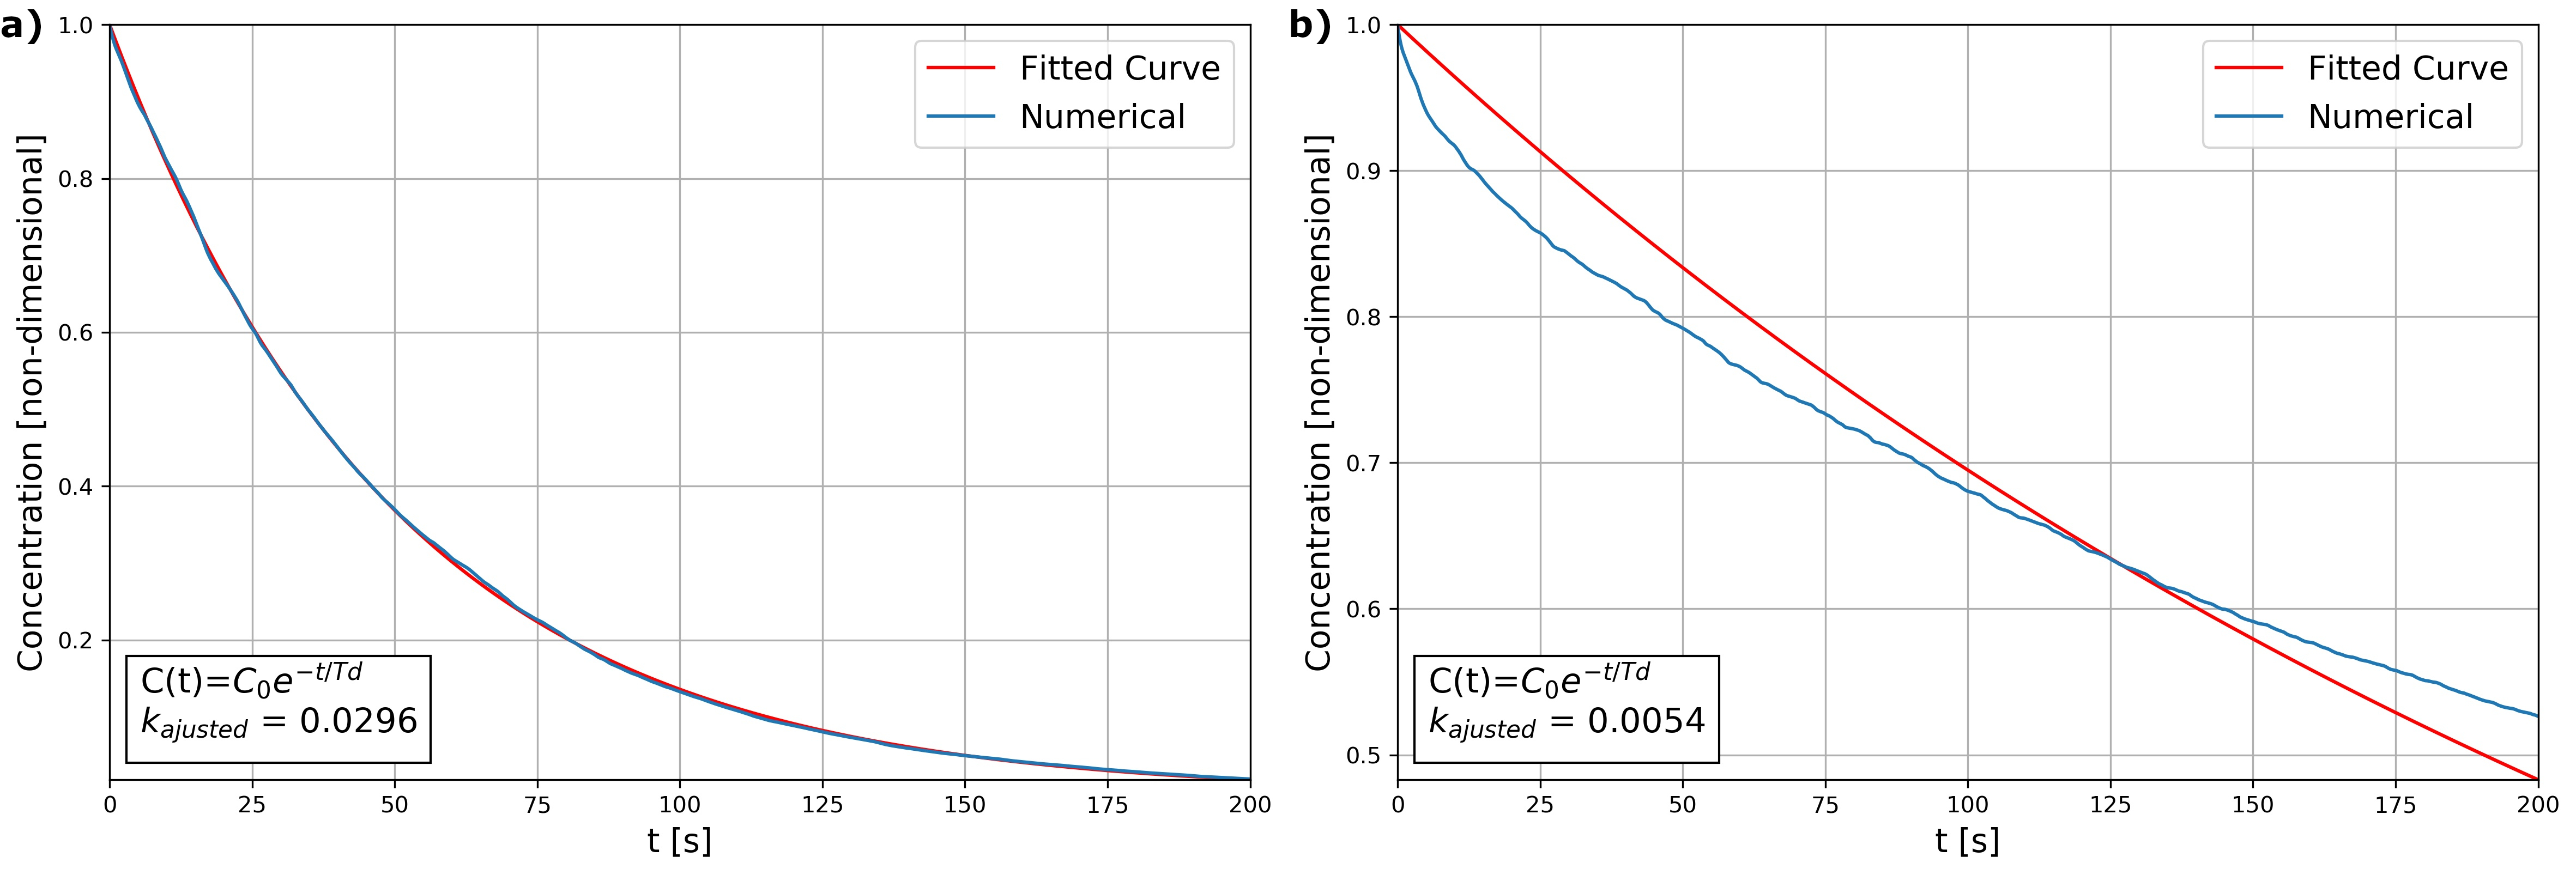
\includegraphics[width=\linewidth]{../images/art4/massDecay.jpeg}
\caption{The variation of the mass exchange coefficient and the mean retention time with the increase of vegetation density.}
\label{fig:art4:massExchange}
\end{figure}

For low-vegetation density ($a < 4$\%), $k$ drops off quickly with increasing vegetation density $a$. For high-vegetation density ($a \geq 4$\%), $k$ is small, but not zero, and decreases slowly with increasing $a$. As the vegetation drag becomes the dominant effect, the velocity within the cavity becomes negligibly small, and it behaves as if the cavity is fully blocked ($\phi = 1$). The mass exchange, then, occurs mainly near the interface volume, this could be an influence of the increase of TKE in the outer part of the mixing layer. The effect of higher TKE levels in the outer mixing layer provides clear water volumes to scratch the vegetation at the interface. As the width of the TKE distribution decreases after a maximum at $a = 5.3380$ \%, the diminishing rate that clear water is available at the interface further slows down the exchange between the zones. Furthermore, the presence of vorticity for $a \leq 7.9920$ indicates that the small vortices could be moving tracer and promoting its diffusion particularly at the inner mixing layer. This behaviour contributed to the mass exchange and the lack of this phenomenon can be seen past $a \geq 7.9920$ when the mass exchange seems to change the asymptote of $k$ decay.

\section{Conclusion}
The hydrodynamics of a single lateral cavity with different vegetation densities was investigated numerically through LES. The results reveal that the single circulation system (non vegetated case) can be transformed into a two-gyre system with the increase of vegetation density. The influence of this secondary gyre decreased the rate in which the mass exchange coefficient diminished.

The dynamic of the flow was examined with both the vorticity and the turbulent kinetic energy (TKE) that both decreased in the downstream direction for all vegetation densities. For $a<2.6640$ \%, the downstream section of the mixing layer has higher values of both TKE and vorticity due to reduced inflow of the shed vortices in the cavity. For $a>2.6640$ \%, these higher values did not appear as the vegetation drag further increased, which is attributable to high blockage effect. The effect of these variables seems to play the dominant effect of the mass exchange in high-density vegetation, as the mass exchange mostly occurs at the inner mixing layer, region where these variables remain not null up to $a=5.3380$ \% for TKE and $a=7.9920$\% for vorticity.

This study enriched the knowledge of interactions between aquatic vegetation and the flow inside a lateral cavity. It shows that vegetation can drastically alter the flow by reducing the velocity, TKE and vorticity, this influence could promote the deposition of fine sediments and organic matter. Furthermore, it shows that the vegetation can cause a threshold in the mass exchange between the main channel and the lateral cavity, in which the rate is drastically reduced due to high blockage effects. This knowledge could help river managers to set limits and adjust the vegetation density inside the cavity in order to keep the desirable ecological function of the cavity.

\addcontentsline{toc}{section}{Funding}
\section*{Funding}
This study was financed in part by the Coordenação de Aperfeiçoamento de Pessoal de Nível Superior - Brazil (CAPES) -Finance Code 001.

This study was partly conducted in Lobo Carneiro cluster located in NACAD/Coppe - Rio de Janeiro, Brazil

\addcontentsline{toc}{section}{References}
\printbibliography[segment=\therefsegment,heading=subbibliography, title={References}]
\chapter{Conclusion and Recommendations}
\label{chap:conclusion}

The objective of this study was the description of the hydrodynamics and mass exchange in dead waters. In the present study, numerical experiments were performed to describe the flow in groynes and lateral cavities.

First, a literature review of the flow conditions and methods used to describe the flow was performed which showed gaps in knowledge to be fulfilled. Second, the first description of the groyne flow was presented along with the study of tracer fields, which showed that the mass exchange between the DZ and the main channel is not unique and occurs at two different rates depending on the elapsed time. Third, the first description of lateral cavities was presented, in this paper, we described the flow using a model developed in commercial software. Forth, the description of lateral cavities was further developed using another approach to the turbulence fields and an open-source package. Finally, the effects of vegetation in lateral cavities were described.

The differences in modelling groynes and lateral cavities are significant. The study of groynes implies a periodicity that must be fulfilled by two means: a) a series of groyne fields or b) a pair of cyclic/periodic surfaces. The difficulties inhered by both methods rely on the high computational cost, as in the option a) the domain is extensive and the meshing process is harder and usually means in a loss of detail as a refined mesh becomes prohibitive. On another hand, the second option provides a more accurate description of the flow as the meshing can be concentrated only on one groyne field, although the implementation of a periodic surface in a zone of high mixture implies in a requirement for a small cell size especially in the groyne head, a region of intense vortex shredding. In contrast to groynes, cavities do not require repetition and can be represented in a simple inlet/outlet scheme, this implies reduced computational costs.

For both studies, as turbulence is the main phenomena in DZ the selection of the turbulence model is primordial to the model. Through the investigation process, it was noticed that the Reynolds Averaging Navier-Stokes can only give an approximation of the flow, we analysed multiple models that rely on this spectra and only the k-$\omega$ SST model was suitable for this kind of flow. Another hybrid model such as the Detached Eddy Simulation was a further improvement to the description of turbulence. Although, some structures were clearer when the Large Eddy Simulation was introduced, as the instantaneous flow was considered.

For vegetated flows, the approximation using porous media to represent the vegetation drag was used. The results of this model proved that this approach is viable for DZ. The effects of the vegetation density in the hydrodynamics and mass exchange proved to follow different phases. The lateral cavity can present a structure that was not anticipated for the given $W/L$ region as a secondary circulation appears when $a>5.3280$\%. This secondary circulation changes how mass is exchanged, similar to the first paper of this dissertation, the exchange values are changed due to the concentration of mass in the secondary gyre that has no contact with the main channel.

This dissertation enriched the knowledge of dead zones vegetated/non-vegetated. It showed different modelling techniques for two types of DZ: lateral cavity and groyne fields. Furthermore, it shows that vegetation can drastically alter the flow by reducing the velocity, TKE and vorticity, this influence could promote the deposition of fine sediments and organic matter. Additionally, it shows that the vegetation can cause a threshold in the mass exchange between the main channel and the lateral cavity, in which the rate is drastically reduced due to high blockage effects. This knowledge could help river managers to set limits and adjust the vegetation density inside the cavity to keep the desirable ecological function of the cavity.


\printbibliography[heading=bibintoc, title={References}]

\begin{appendices}
\chapter{Total Turbulent Kinetic Energy Function}
\label{chap:appendixA}
\noindent As the default function to write the TKE values does not account for the instantaneous values generated from the LES model, a new function was written to account both the instantaneous and averaged values. The code of the function totalTKE calculates the TKE based on the Resolved Reynolds Stress Tensor took from the instantaneous fluctuation of the velocity ($u'$) and the Subgrid Reynolds Stress Tensor ($R$).
\begin{equation}
totalTKE= 0.5tr(R) + 0.5tr(u')
\end{equation}
\begin{lstlisting}
totalTKE
{
	type			coded;
	libs			("libutilityFunctionObjects.so");
	name			totalTKE;
	executeControl	timeStep;
	writeControl	writeTime;
	timeStart		155;
	enabled			true;

/*---------------------------------------------------------------------------*\

	Total Turbulent Kinect Energy Evaluation
		** Requires fieldAverage Function to Obtain UPrime2Mean**
			** Resolved Reynolds Stress Tensor
		** Requires turbulenceFields Function to Obtain R**
			** Subgrid Reynolds Stress Tensor

\*---------------------------------------------------------------------------*/

	codeExecute
	#{
		static autoPtr<volScalarField> totalTKE;

		if
		(
			mesh().foundObject<volSymmTensorField>("UPrime2Mean")
			&&
			mesh().foundObject<volSymmTensorField>("turbulenceProperties:R")
			&&
			mesh().foundObject<volScalarField>("totalTKE") == 0
		)
		{
			Info << "Turbulent Kinect Energy:" << endl;
			Info << "	Initialising" << endl;
			Info << "	Calculating" << nl << endl;

			totalTKE.set
			(
				new volScalarField
				(
					IOobject
					(
						"totalTKE",
						mesh().time().timeName(),
						mesh(),
						IOobject::NO_READ,
						IOobject::AUTO_WRITE
					),
					mesh(),
					dimensionedScalar
					(
						"totalTKE",
						dimensionSet(0,2,-2,0,0,0,0),
						0
					)
				)
			);

			const volSymmTensorField& R = mesh().lookupObjectRef<volSymmTensorField>("turbulenceProperties:R");
			const volSymmTensorField& UPrime2Mean = mesh().lookupObjectRef<volSymmTensorField>("UPrime2Mean");

			volScalarField& totalTKE = mesh().lookupObjectRef<volScalarField>("totalTKE");
			totalTKE = (0.5 * tr(R)) + (0.5 * tr(UPrime2Mean));
		}

		else if
		(
			mesh().foundObject<volSymmTensorField>("UPrime2Mean")
			&&
			mesh().foundObject<volSymmTensorField>("turbulenceProperties:R")
			&&
			mesh().foundObject<volScalarField>("totalTKE")
		)
		{
			Info << "Turbulent Kinect Energy:" << endl;
			Info << "	Calculating" << nl << endl;

			const volSymmTensorField& R = mesh().lookupObjectRef<volSymmTensorField>("turbulenceProperties:R");
			const volSymmTensorField& UPrime2Mean = mesh().lookupObjectRef<volSymmTensorField>("UPrime2Mean");

			volScalarField& totalTKE = mesh().lookupObjectRef<volScalarField>("totalTKE");
			totalTKE = (0.5 * tr(R)) + (0.5 * tr(UPrime2Mean));
		}

		else
		{
			Info << "Turbulent Kinect Energy:" << endl;
			Warning << endl
					<< "	Unable to Calculate Turbulent Kinect Energy" << endl
					<< "	UPrime2Mean and/or R Unavailable" << endl
					<< "	Enable fieldAverage and turbulenceFields Functions" << nl << endl;
		}
	#};
}
\end{lstlisting}

\chapter{Data Processing}
\label{chap:appendixB}
\noindent
In this appendix the script used to process simulation data is presented. This code uses python to calculate the ensemble averaging properties in a 2D plane. Note, the only process that is not fully automated is the calculation of the mixing length that requires the user to manually fill the maximum value of the absolute velocity gradient in the y direction $({\partial \bar u}/{\partial y})_{max}$.

\section{File Structure}
\noindent
The file structure of the script is shown bellow:
\\
\dirtree{%
.1 /.
.2 bin.
.3 dataProcess.py\DTcomment{Data Analysing and Exporting script}.
.3 importCSV.py\DTcomment{CSV import script}.
.3 mass.py\DTcomment{Mass analysis script}.
.3 plot.py\DTcomment{Plotting script}.
.3 multipleSimulationImport.py\DTcomment{CSV import script}.
.3 multipleSimulationProcess.py\DTcomment{Velocity Analysis script}.
.3 multipleSimulationPlot.py\DTcomment{Plotting and export script}.
.3 thickness\DTcomment{Calculation of the thickness of the mixing layer}.
.2 dataset\DTcomment{Directory with literature data}.
.2 treatment\DTcomment{Directory for multiple simulations treatment}.
.3 results\DTcomment{Software Created Directory}.
.2 preTreatment\DTcomment{Directory for a single simulation treatment}.
.3 results\DTcomment{Software Created Directory}.
.2 preProcessing.py.
.2 dataAnalysis.py.
}
\noindent

The requirements of the script are:
\begin{itemize}
\item Python 3.x
\item Scipy
\item Numpy
\item Pandas
\item Matplotlib
\end{itemize}
\noindent

\section{preProcessing.py}
The execution of the preProcessing.py script depends on the preTreatment directory that contains the .csv files to be analysed and the dataset directory that contains the csv extracted from literature.

\begin{lstlisting}[language=python]
#!/usr/bin/env python3
# -*- coding: utf-8 -*-
#
#  preProcessing.py
#  
#  Copyright 2020 Luiz Oliveira
#  
#  This program is free software; you can redistribute it and/or modify
#  it under the terms of the GNU General Public License as published by
#  the Free Software Foundation; either version 2 of the License, or
#  (at your option) any later version.
#  
#  This program is distributed in the hope that it will be useful,
#  but WITHOUT ANY WARRANTY; without even the implied warranty of
#  MERCHANTABILITY or FITNESS FOR A PARTICULAR PURPOSE.  See the
#  GNU General Public License for more details.
#  
#  You should have received a copy of the GNU General Public License
#  along with this program; if not, write to the Free Software
#  Foundation, Inc., 51 Franklin Street, Fifth Floor, Boston,
#  MA 02110-1301, USA.
#  
#  

"""
Main module

This script analyses the output of simulations ran on OpenFoam
The analysis steps are performed by the modules in the bin folder
"""

import sys
import os
import shutil
import time
start_time = time.time()

# Check for necessary directories
if not os.path.exists('preTreatment'):
    os.makedirs('preTreatment')
    print("The directory preTreatment/ was created, please populate with the "
          "desired csv files to be analysed.")
    sys.exit('The directory preTreatment/ did not exist.')
elif not os.listdir('preTreatment'):
    sys.exit('The directory preTreatment/ is empty.')
    
# Clear the previous results directories
if os.path.exists('preTreatment/results'):
    shutil.rmtree('preTreatment/results')
os.makedirs('preTreatment/results')
os.makedirs('preTreatment/results/Excel')
os.makedirs('preTreatment/results/CSV')
os.makedirs('preTreatment/results/Plot')

# Define Global Variables
H = 0.10
U = 0.101
W = 0.15
L = 0.25
Y0 = 0.30
X0 = 0.25
RHO = 1e-6

# Import CSV
exec(open("bin/importCSV.py").read())
print("""Importing Done...
Elapsed Time %.3f s\n""" %(time.time() - start_time))

# Data Processing
try:
    exec(open("bin/dataProcess.py").read())
    print("""Processing Done...
Elapsed Time %.3f s\n""" %(time.time() - start_time))
except:
    print("""No data was processed.
The script jumped into the next section: Mass Fitting""")
    print("Elapsed Time %.3f s\n" %(time.time() - start_time))

# Mass Fitting
try: 
    exec(open("bin/mass.py").read())
    print("""Mass Fitting Done...
Elapsed Time %.3f s\n""" %(time.time() - start_time))
except:
    print("""No mass data was processed.
The script jumped into the next section: Mixing Layer Thickness""")
    print("Elapsed Time %.3f s\n" %(time.time() - start_time))
    
# Mixing Layer Thickness
try: 
    exec(open("bin/thickness.py").read())
    print("""Mixing Layer Thickness Calculated...
Elapsed Time %.3f s\n""" %(time.time() - start_time))
except:
    print("""No mixing layer thickness data was processed.
The script jumped into the next section: Plotting""")
    print("Elapsed Time %.3f s\n" %(time.time() - start_time))
    
# Plot Data
try:
    exec(open("bin/plot.py").read())
    print("""Plotting Done...
Elapsed Time %.3f s\n""" %(time.time() - start_time))
except:print("No plotting was done.\n")

print("""All Done...
Execution Time %.3f seconds""" %(time.time() - start_time))
del start_time

\end{lstlisting}
\section{dataAnalysis.py}
\noindent
The execution of the dataAnalysis.py script depends on the treatment directory that contains the .csv files to be analysed. These files must be pre processed using the previous script.
\begin{lstlisting}[language=python]
#!/usr/bin/env python3
# -*- coding: utf-8 -*-
#
#  dataAnalysis.py
#
#  Copyright 2020 Luiz Oliveira <luiz@luizLinux>
#
#  This program is free software; you can redistribute it and/or modify
#  it under the terms of the GNU General Public License as published by
#  the Free Software Foundation; either version 2 of the License, or
#  (at your option) any later version.
#
#  This program is distributed in the hope that it will be useful,
#  but WITHOUT ANY WARRANTY; without even the implied warranty of
#  MERCHANTABILITY or FITNESS FOR A PARTICULAR PURPOSE.  See the
#  GNU General Public License for more details.
#
#  You should have received a copy of the GNU General Public License
#  along with this program; if not, write to the Free Software
#  Foundation, Inc., 51 Franklin Street, Fifth Floor, Boston,
#  MA 02110-1301, USA.
#
#
"""
Main module

This script analyses the output of preProcessing.py
The analysis steps are performed by the modules in the bin folder
"""

import sys
import os
import shutil
import time
start_time = time.time()

# Check for necessary directories
if not os.path.exists('treatment'):
    os.makedirs('treatment')
    print("The directory treatment/ was created, please populate with the "
          "desired csv files to be analysed.")
    sys.exit('The directory treatment/ did not exist.')
elif not os.listdir('treatment'):
    sys.exit('The directory treatment/ is empty.')

# Clear the previous results directories
if os.path.exists('treatment/results'):
    shutil.rmtree('treatment/results')
os.makedirs('treatment/results')
os.makedirs('treatment/results/Plots')
os.makedirs('treatment/results/SelectPlots')
os.makedirs('treatment/results/CSV')

# Define Global Variables
H = 0.10
U = 0.101
W = 0.15
L = 0.25
Y0 = 0.30
X0 = 0.25
RHO = 1e-6

# Import CSV
exec(open("bin/multipleSimulationImport.py").read())
print("""Importing Done...
Elapsed Time %.3f s\n""" %(time.time() - start_time))

# Process Data
exec(open("bin/multipleSimulationProcess.py").read())
print("""Processing Done...
Elapsed Time %.3f s\n""" %(time.time() - start_time))

# Data plot
exec(open("bin/multipleSimulationPlot.py").read())
print("""Plotting Done...
Elapsed Time %.3f s\n""" %(time.time() - start_time))

print("""All Done...
Execution Time %.3f seconds""" %(time.time() - start_time))
del start_time

\end{lstlisting}
\section{preProcessing Scripts}
\subsection{importCSV.py}
\begin{lstlisting}[language=python]
#!/usr/bin/env python3
# -*- coding: utf-8 -*-
#
#  importCSV.py
#  
#  Copyright 2020 Luiz Oliveira
#  
#  This program is free software; you can redistribute it and/or modify
#  it under the terms of the GNU General Public License as published by
#  the Free Software Foundation; either version 2 of the License, or
#  (at your option) any later version.
#  
#  This program is distributed in the hope that it will be useful,
#  but WITHOUT ANY WARRANTY; without even the implied warranty of
#  MERCHANTABILITY or FITNESS FOR A PARTICULAR PURPOSE.  See the
#  GNU General Public License for more details.
#  
#  You should have received a copy of the GNU General Public License
#  along with this program; if not, write to the Free Software
#  Foundation, Inc., 51 Franklin Street, Fifth Floor, Boston,
#  MA 02110-1301, USA.
#  
#  

"""
Data is imported from text files to be later processed and ploted
"""

# Libraries
import os
import re
import pandas as pd

# Import Literature
literatureExp = pd.read_csv('dataset/fig4/fig4a.csv', header = 1, usecols=(0,1))
literatureExp.columns = ['(y-y0)/H','u/U']
literatureExp = literatureExp.dropna()
literatureLES = pd.read_csv('dataset/fig4/fig4a.csv', header = 1, usecols=(2,3))
literatureLES.columns = ['(y-y0)/H','u/U']
massLiterature = pd.read_csv('dataset/mass/mass.csv', header = 1)
massLiterature.columns = ['Vegetation Density', 'Td']
massLiterature.Td = massLiterature.Td * U / H

# Tracer data
try:
    tracerData = pd.read_csv('preTreatment/tracerVolAve.dat',
                             delimiter='\t', header = 3)
    tracerData.columns = ['time', 'tracerVol']
    tracerData.tracerVol[0] = 1
    massTimeZero = tracerData.time[0]
    tracerData.time = tracerData.time - massTimeZero
except:pass

# Partial Tracer at Interface
try:
    interfaceTracer = dict()
    regions = ['Bottom', 'Middle', 'Top']
    for reg in regions:
        interfaceTracer[reg] = pd.read_csv('preTreatment/tracer'+reg+'.dat',\
                                            delimiter='\t', header = 4)
        interfaceTracer[reg].columns = ['time', 'tracer']
        interfaceTracer[reg].time = interfaceTracer[reg].time - massTimeZero
    Eraw = pd.read_csv('preTreatment/velocityInterface.dat', delimiter='\t',\
                    header = 4)
    Eraw.columns = ['time', 'absVelInt']
    Eraw.time = Eraw.time - massTimeZero
    Eraw.absVelInt = Eraw.absVelInt/(2*H*L)
except:pass

# Generic Planes
files = os.listdir('preTreatment')

# Check for csv files
rawFiles = list()
csvFiles = list()
datFiles = list()
uniqueRaw = list()
uniqueVar = list()

# Removes ':' from file name
for item in files:
    if ':' in item:    
        newname = item.split(':')[1]
        os.rename('preTreatment/'+item, 'preTreatment/'+newname)
        
files = os.listdir('preTreatment')

for item in files:
      if re.search('.\.raw', item):
          rawFiles.append(item)

for item in files:
      if re.search('.\.csv', item):
          csvFiles.append(item)
          
for item in files:
      if re.search('.\.dat', item):
          datFiles.append(item)

csvFiles.sort() 
datFiles.sort() 
rawFiles.sort()

for item in rawFiles:
    try:
        plane = re.findall("_([\d\D]..)", item)[0]
        variableName = re.split("_", item)[0]
        if plane not in uniqueRaw:
            uniqueRaw.append(plane)
        if variableName not in uniqueVar:
            uniqueVar.append(variableName)
    except:continue

def cleanHeader(name):
    fh = open('preTreatment/'+name, "rt")
    data = fh.read()
    # data = re.sub(r':\S+ ', r'', data)
    data = data.replace('# ', '')
    data = data.replace('  ', ' ') #removes double spacing
    
    fh.close()
    fh = open('preTreatment/'+name, "wt")
    fh.write(data)
    fh.close()

# Import generated data
for item in rawFiles:
    for item2 in uniqueRaw:
        try:
            plane = re.findall("_([\d\D]..)", item)[0]
            if plane == item2:
                cleanHeader(item)
                variableName = re.split("_", item)[0]
                aux = pd.read_csv('preTreatment/'+item, sep=" ", header=1,
                                  float_precision="high",skipinitialspace=True)
                #if aux.isnull().values.any():continue
                try:
                    if variableName not in locals():vars()[variableName] = aux
                    else:
                        vars()[variableName] = pd.concat([vars()[variableName],aux],
                                              ignore_index=True, axis=1)
                        vars()[variableName] = vars()[variableName].dropna(axis=0, how='all')
                        vars()[variableName] = vars()[variableName].dropna(axis=1, how='all')
                except:continue
        except:continue

thickness = dict()
for item in csvFiles:
    try:
        thickness['raw'] = pd.read_csv('preTreatment/'+item, header=0,\
                                float_precision='high')
        if len(thickness['raw'].columns) == 8:
            thickness['raw'].drop(['Gradients_0','Gradients_1','Gradients_2'],\
                     axis=1, inplace=True)
        colNames = ['x', 'y', 'z', 'UMean_X', 'absGradient']
        thickness['raw'].columns = colNames
        
        del colNames
    except:continue

try:
    del aux, variableName, item2, plane
except:pass

del files, item, rawFiles, csvFiles, reg

\end{lstlisting}

\subsection{dataProcess.py}
\begin{lstlisting}[language=python]
#!/usr/bin/env python3
# -*- coding: utf-8 -*-
#
#  dataProcess.py
#  
#  Copyright 2020 Luiz Oliveira
#  
#  This program is free software; you can redistribute it and/or modify
#  it under the terms of the GNU General Public License as published by
#  the Free Software Foundation; either version 2 of the License, or
#  (at your option) any later version.
#  
#  This program is distributed in the hope that it will be useful,
#  but WITHOUT ANY WARRANTY; without even the implied warranty of
#  MERCHANTABILITY or FITNESS FOR A PARTICULAR PURPOSE.  See the
#  GNU General Public License for more details.
#  
#  You should have received a copy of the GNU General Public License
#  along with this program; if not, write to the Free Software
#  Foundation, Inc., 51 Franklin Street, Fifth Floor, Boston,
#  MA 02110-1301, USA.
#  
#  
"""
This code processes the data imported from importcsv.py
The data is ensembled averaged and then exported to plot.py script
"""

import re
import pandas as pd
import openpyxl
from scipy.interpolate import interp1d

def dfRename(var, dtf):
    names = ['x', 'y', 'z']
    names.extend(var)
    dtf.columns = names

def clearLimits(df,x0,x1,y0,y1,z0,z1):
# =============================================================================
#     Clear extra values inside variables.
#     This script uses user values of the bound coordinates
# =============================================================================

    df.drop(df[df.x < x0].index, inplace=True)
    df.drop(df[df.x > x1].index, inplace=True)
    df.drop(df[df.y < y0].index, inplace=True)
    df.drop(df[df.y > y1].index, inplace=True)
    df.drop(df[df.z < z0].index, inplace=True)
    df.drop(df[df.z > z1].index, inplace=True)
    return df

def excelExport(var, name):
# =============================================================================
#     Creates and appends planes into an spreadsheet
# =============================================================================
    
    if not os.path.isfile('preTreatment/results/Excel/'+name+'.xlsx'):
        wb = openpyxl.Workbook()
        wb.save('preTreatment/results/Excel/'+name+'.xlsx')

    with pd.ExcelWriter('preTreatment/results/Excel/'+name+'.xlsx',
                        engine="openpyxl", mode='a') as writer:
        for df_name, df in var.items():
            df.to_excel(writer, sheet_name=df_name, index=False)
            
def csvExport(df, name):
# =============================================================================
#     Creates and appends planes into separated csv files
# =============================================================================
    df.to_csv('preTreatment/results/CSV/'+name+'.csv')

def varTreatment(planes, physicalVar, colNames, nColumns, direction,
                 varName, roundPar, first, last):
# =============================================================================
#     Treats data in an ensemble averaging proceedure in the provided direction
# =============================================================================

    # Local Variable Declaration
    varDict = dict()
    kk = first * nColumns
    startPos = first
    stopPos = last * nColumns
    ll = 0
  
    # Reads all the files and ensemble in a dict in that each ii is a plane
    for ii in planes:
        key = ii
        key = int(re.sub('\D', '',key))
        if key < startPos:
            continue
        if kk > stopPos: 
            break
        for jj in range(nColumns):
            ll = kk + jj
            if ll%nColumns == 0: # number of columns
                varDict[ii] = physicalVar.iloc[:,ll]
            else:
                varDict[ii] = \
                    pd.concat([varDict[ii], physicalVar.iloc[:,ll]], axis=1)
                    
        kk = kk + nColumns

        dfRename(colNames, varDict[ii])
        clearLimits(varDict[ii], 0.25, 0.50, 0.30, 0.45, 0, 0.1)
        varDict[ii] = varDict[ii].dropna(axis=0, how='all')
        varDict[ii] = varDict[ii].dropna(axis=1, how='all')

        # Get vector magnitude
        if nColumns > 4:
            df = pd.DataFrame()
            for i in colNames:
                df[i] = varDict[ii][i]**2
            df['mag'] = (df.sum(axis=1))**(1/2)
            varDict[ii]['mag'] = df.mag
            expColNames = colNames + ['mag']
        else:
            expColNames = colNames
            
        if direction == "x":
            varDict[ii] = varDict[ii].drop(columns=['y', 'z'])
            varDict[ii] = varDict[ii].\
            groupby(varDict[ii].x.round(roundPar),as_index=False).mean()
            varDict[ii][direction] = (varDict[ii][direction] - 0.25)/L
            varDict[ii].columns = ['('+direction+'-x0)'+'/L'] + expColNames
        elif direction == 'y':
            varDict[ii] = varDict[ii].drop(columns=['x', 'z'])
            varDict[ii] = varDict[ii].\
            groupby(varDict[ii].y.round(roundPar),as_index=False).mean()
            varDict[ii][direction] = (varDict[ii][direction] - 0.30)/H
            varDict[ii].columns = ['('+direction+'-y0)'+'/H'] + expColNames
        elif direction == 'z':
            varDict[ii] = varDict[ii].drop(columns=['x', 'y'])
            varDict[ii] = varDict[ii].\
            groupby(varDict[ii].z.round(roundPar),as_index=False).mean()
            varDict[ii][direction] = varDict[ii][direction]/H
            varDict[ii].columns = [direction+'/H'] + expColNames
            
        excelExport(varDict, varName+"Dir_"+direction)
        csvName = varName.split("_")[0]
        csvExport(varDict[ii], csvName+"_"+ii+"_Dir_"+direction)
    return varDict


# =============================================================================
# Planes 0 -> 4
# Vertical Planes Varying the Y axis from Y = 0.30 to Y = 0.45
# =============================================================================
## RMean
colNames = ['xx', 'yy', 'zz', 'xy', 'yz', 'xz']
RMean_00_04_Dirx = varTreatment(uniqueRaw, RMean, colNames, 9,'x',
                               'RMean_00_4_',2, 0, 4)
RMean_00_04_Dirz = varTreatment(uniqueRaw, RMean, colNames, 9,'z',
                               'RMean_00_4_',2, 0, 4)

## UMean
colNames = ['u', 'v', 'w']
UMean_00_04_Dirx = varTreatment(uniqueRaw, UMean, colNames, 6,'x',
                               'UMean_00_4_',2, 0, 4)
UMean_00_04_Dirz = varTreatment(uniqueRaw, UMean, colNames, 6,'z',
                               'UMean_00_4_',2, 0, 4)

## lambVectorMean
colNames = ['lambVectorMean_x', 'lambVectorMean_y', 'lambVectorMean_z']
lambVectorMean_00_04_Dirx = varTreatment(uniqueRaw, lambVectorMean, colNames, 6,
                                    'x','lambVectorMean_00_4_',3, 0, 4)
lambVectorMean_00_04_Dirz = varTreatment(uniqueRaw, lambVectorMean, colNames,
                                    6,'z','lambVectorMean_00_4_',2, 0, 4)

## pMean
colNames = ['pMean']
pMean_00_04_Dirx = varTreatment(uniqueRaw, pMean, colNames, 4,'x',
                               'pMean_00_4_',3, 0, 4)
pMean_00_04_Dirz = varTreatment(uniqueRaw, pMean, colNames, 4,'z',
                               'pMean_00_4_',2, 0, 4)

## vorticityMean
colNames = ['vorticityMean_x', 'vorticityMean_y', 'vorticityMean_z']
vorticityMean_00_04_Dirx = varTreatment(uniqueRaw, vorticityMean, colNames, 6,
                                  'x','vorticityMean_00_4_',3, 0, 4)
vorticityMean_00_04_Dirz = varTreatment(uniqueRaw, vorticityMean, colNames, 6,
                                  'z','vorticityMean_00_4_',2, 0, 4)

# =============================================================================
# Planes 5 -> 11
# Vertical Planes Varying the X axis from X = 0.25 to X = 0.50
# =============================================================================
## RMean
colNames = ['xx', 'yy', 'zz', 'xy', 'yz', 'xz']
RMean_05_11_Diry = varTreatment(uniqueRaw, RMean, colNames, 9,'y',
                                'RMean_05_11_',2, 5, 11)
RMean_05_11_Dirz = varTreatment(uniqueRaw, RMean, colNames, 9,'z',
                                'RMean_05_11_',2, 5, 11)

## UMean
colNames = ['u', 'v', 'w']
UMean_05_11_Diry = varTreatment(uniqueRaw, UMean, colNames, 6,'y',
                                'UMean_05_11_',2, 5, 11)
UMean_05_11_Dirz = varTreatment(uniqueRaw, UMean, colNames, 6,'z',
                                'UMean_05_11_',2, 5, 11)

## lambVectorMean
colNames = ['lambVectorMean_x', 'lambVectorMean_y', 'lambVectorMean_z']
lambVectorMean_05_11_Diry = varTreatment(uniqueRaw, lambVectorMean, colNames, 6,
                                    'y','lambVectorMean_05_11_',3, 5, 11)
lambVectorMean_05_11_Dirz = varTreatment(uniqueRaw, lambVectorMean, colNames,
                                    6,'z','lambVectorMean_05_11_',2, 5, 11)

## pMean
colNames = ['pMean']
pMean_05_11_Diry = varTreatment(uniqueRaw, pMean, colNames, 4,'y',
                                'pMean_05_11_',3, 5, 11)
pMean_05_11_Dirz = varTreatment(uniqueRaw, pMean, colNames, 4,'z',
                                'pMean_05_11_',2, 5, 11)

## vorticityMean
colNames = ['vorticityMean_x', 'vorticityMean_y', 'vorticityMean_z']
vorticityMean_05_11_Diry = varTreatment(uniqueRaw, vorticityMean, colNames, 6,
                                  'y','vorticityMean_05_11_',3, 5, 11)
vorticityMean_05_11_Dirz = varTreatment(uniqueRaw, vorticityMean, colNames, 6,
                                  'z','vorticityMean_05_11_',2, 5, 11)

# =============================================================================
# Planes 12 -> 21
# Horizontal Planes Varying the Z axis from Z = 0 to Z = 0.10
# =============================================================================
## RMean
colNames = ['xx', 'yy', 'zz', 'xy', 'yz', 'xz']
RMean_12_21_Dirx = varTreatment(uniqueRaw, RMean, colNames, 9,'x',
                                'RMean_12_21_',2, 12, 21)
RMean_12_21_Diry = varTreatment(uniqueRaw, RMean, colNames, 9,'y',
                                'RMean',2, 12, 21)

## UMean
colNames = ['u', 'v', 'w']
UMean_12_21_Dirx = varTreatment(uniqueRaw, UMean, colNames, 6,'x',
                                'UMean_12_21_',2, 12, 21)
UMean_12_21_Diry = varTreatment(uniqueRaw, UMean, colNames, 6,'y',
                                'UMean_12_21_',2, 12, 21)

## lambVectorMean
colNames = ['lambVectorMean_x', 'lambVectorMean_y', 'lambVectorMean_z']
lambVectorMean_12_21_Dirx = varTreatment(uniqueRaw, lambVectorMean, colNames, 6,
                                    'x','lambVectorMean_12_21_',3, 12, 21)
lambVectorMean_12_21_Diry = varTreatment(uniqueRaw, lambVectorMean, colNames,
                                    6,'y','lambVectorMean_12_21_',2, 12, 21)

## pMean
colNames = ['pMean']
pMean_12_21_Dirx = varTreatment(uniqueRaw, pMean, colNames, 4,'x',
                                'pMean_12_21_',3, 12, 21)
pMean_12_21_Diry = varTreatment(uniqueRaw, pMean, colNames, 4,'y',
                                'pMean_12_21_',2, 12, 21)

## vorticityMean
colNames = ['vorticityMean_x', 'vorticityMean_y', 'vorticityMean_z']
vorticityMean_12_21_Dirx = varTreatment(uniqueRaw, vorticityMean, colNames, 6,
                                  'x','vorticityMean_12_21_',3, 12, 21)
vorticityMean_12_21_Diry = varTreatment(uniqueRaw, vorticityMean, colNames, 6,
                                  'y','vorticityMean_5_11_',2, 12, 21)

# =============================================================================
# Validation Data
# =============================================================================
## Data Treatment
colNames = ['u', 'v', 'w']
fig4aOur = varTreatment(['p17'], UMean, colNames, 6, "y",'UMean_p17_',
                            3, 17, 17)
fig4aOur = fig4aOur['p17']
fig4aOur.u = fig4aOur.u/U

# Errors from experimental
error = dict()
error['X'] = literatureExp.iloc[:,0]
error['Numerical_u'] = interp1d(fig4aOur.iloc[:,0],fig4aOur.u)(literatureExp.iloc[:,0])
error['Experimental_u'] = literatureExp.iloc[:,1]

error = pd.DataFrame(data=error)
error.eval('Error = Experimental_u - Numerical_u', inplace=True)
error.eval('Abs_Error = abs(Experimental_u - Numerical_u)', inplace=True)
error.eval('Rel_Error = (Experimental_u - Numerical_u)/Experimental_u', inplace=True)
error.eval('Abs_Rel_Error = abs((Experimental_u - Numerical_u)/Experimental_u)', inplace=True)

description = error.describe()

if not os.path.isfile('preTreatment/results/Excel/validationData.xlsx'):
    wb = openpyxl.Workbook()
    wb.save('preTreatment/results/Excel/validationData.xlsx')

with pd.ExcelWriter('preTreatment/results/Excel/validationData.xlsx',
                    engine="openpyxl", mode='a') as writer:
    error.to_excel(writer, sheet_name='Errors', index=False)
    description.to_excel(writer, sheet_name='Statistical Description')

del lambVectorMean, pMean, RMean, vorticityMean, colNames

\end{lstlisting}

\subsection{mass.py}
\begin{lstlisting}[language=python]
#!/usr/bin/env python3
# -*- coding: utf-8 -*-
#
#  mass.py
#  
#  Copyright 2020 Luiz Oliveira
#  
#  This program is free software; you can redistribute it and/or modify
#  it under the terms of the GNU General Public License as published by
#  the Free Software Foundation; either version 2 of the License, or
#  (at your option) any later version.
#  
#  This program is distributed in the hope that it will be useful,
#  but WITHOUT ANY WARRANTY; without even the implied warranty of
#  MERCHANTABILITY or FITNESS FOR A PARTICULAR PURPOSE.  See the
#  GNU General Public License for more details.
#  
#  You should have received a copy of the GNU General Public License
#  along with this program; if not, write to the Free Software
#  Foundation, Inc., 51 Franklin Street, Fifth Floor, Boston,
#  MA 02110-1301, USA.
#  
#  

"""
Mass quantities are analysed in two ways: by tracer volume and y-velocity
"""

# Libraries
from datetime import datetime
import numpy as np
import pandas as pd
import openpyxl
from scipy.optimize import curve_fit


# Extracting date for report
now = datetime.now()
today = now.strftime("%d/%m/%Y %H:%M:%S")

# Define Fitting Function
def model(x, td):
    """
    First Order Mass Decay Equation
    """
    return np.exp(-x/td)

td, pcov = curve_fit(model, tracerData.time, tracerData.tracerVol, p0=(40),
                     maxfev=5000)

k = W / (td * U)

modelmass = model(tracerData.time, td)

tdExp = massLiterature.iloc[1,1]

tdRelError = ((td - tdExp)/tdExp)*100
tdAbsError = tdExp - td

kexp = W / (tdExp * U) # Non-dimensional experimental value
kRelError = ((k - kexp)/kexp)*100
kAbsError = kexp - k

# Mass as function of velocity
E = Eraw.absVelInt.mean()

tdvel = W/E
kvel = W / (tdvel * U)

# Mass Summary
file = open("preTreatment/results/massExchange.txt","w")
file.write("Mass Exchange Values (Simulated - Tracer)\n")
file.write("ktracer = %.4f\n" %k)
file.write("Mean Residence Time = %.2f\n---\n" %td)
file.write("Mass Exchange Values (Simulated - Interface Velocity)\n")
file.write("kvelocity = %.4f\n" %kvel)
file.write("Mean Residence Time = %.2f\n---\n" %tdvel)
file.write("Mass Exchange Values (Xiang)\n")
file.write("kexp = %.4f\n" %kexp)
file.write("Mean Residence Time = %.2f\n---\n" %tdExp)
file.write("Error analysis\n")
file.write("Relative error\n")
file.write("\tError = (Simulated.our - Xiang)/(Xiang)\n")
file.write("MRT = %.2f %%\n" %tdRelError)
file.write("k = %.2f %%\n" %kRelError)
file.write("Absolute error\n")
file.write("MRT = %.2f\n" %tdAbsError)
file.write("k = %.2f\n" %kAbsError)
file.write("---\nData analysed in {} (GMT-4)".format(today))
file.close()

# Construct mass dataFrame
tracerDataExport = tracerData
tracerDataExport['modelled'] = modelmass
colNames = ['Time','Numerical','Modelled']
tracerDataExport.columns = colNames

tracerDataExport.to_csv('preTreatment/results/CSV/tracerData.csv')
with pd.ExcelWriter('preTreatment/results/Excel/tracerData.xlsx',
                    engine="openpyxl", mode='w') as writer:
    for df_name, df in tracerDataExport.items():
        df.to_excel(writer, sheet_name=df_name, index=False)
        
del file, now, today

\end{lstlisting}
\subsection{plot.py}
\begin{lstlisting}[language=python]
#!/usr/bin/env python3
# -*- coding: utf-8 -*-
#
#  plot.py
#  
#  Copyright 2020 Luiz Oliveira
#  
#  This program is free software; you can redistribute it and/or modify
#  it under the terms of the GNU General Public License as published by
#  the Free Software Foundation; either version 2 of the License, or
#  (at your option) any later version.
#  
#  This program is distributed in the hope that it will be useful,
#  but WITHOUT ANY WARRANTY; without even the implied warranty of
#  MERCHANTABILITY or FITNESS FOR A PARTICULAR PURPOSE.  See the
#  GNU General Public License for more details.
#  
#  You should have received a copy of the GNU General Public License
#  along with this program; if not, write to the Free Software
#  Foundation, Inc., 51 Franklin Street, Fifth Floor, Boston,
#  MA 02110-1301, USA.
#  
#  

"""
Data is imported from dataProcess.py and ploted into png figures
"""

# Libraries
import re
import matplotlib.pyplot as plt
from matplotlib import ticker
from matplotlib.offsetbox import AnchoredText

def plotVar(varName, axis, title, name, col, admensional, first, last):
# =============================================================================
#     Runs through all plots from a variable and plots it
# =============================================================================
    fig, ax = plt.subplots(figsize=(9,6), dpi=300)

    for key, df in varName.items():
        nKey = key
        nKey = int(re.sub('\D', '',nKey))
        if nKey >= first and nKey <= last:
            if 'z' not in varName[key].iloc[:,0].name:
                ax.plot(varName[key].iloc[:,0],
                        varName[key].iloc[:,col]/admensional, label=key)
            else:
                ax.plot(varName[key].iloc[:,col]/admensional,
                        varName[key].iloc[:,0], label=key)

    ax.legend(loc='best',fontsize='x-large')
    if title != "None":
        ax.set_title(title,fontsize='xx-large')

    plt.grid()
    plt.autoscale(enable=True, tight=True)
    plt.xlabel(axis[0],fontsize='x-large')
    plt.ylabel(axis[1],fontsize='x-large')
    plt.savefig('preTreatment/results/Plot/'+name+'.png', bbox_inches='tight',
                format='png')
    plt.close()

# =============================================================================
# Planes 0 -> 4
# Vertical Planes Varying the Y axis from Y = 0.30 to Y = 0.45
# =============================================================================

noTitle = "None"
    
## RMean Dir_x_00_04
axisNames = ['(x-x0)/L','Rmag/U2']
plotTitle = 'Time Averaged Reynolds Stresses Magnitude at vertical XZ planes'
figureName = 'RMean_mag_Dir_x_00_04'
plotVar(RMean_00_04_Dirx, axisNames, noTitle, figureName, 7, U**2, 0, 4)

## RMean Dir_x_00_04
axisNames = ['Rmag/U2', 'z/H']
plotTitle = 'Time Averaged Reynolds Stresses Magnitude at vertical XZ planes'
figureName = 'RMean_mag_Dir_x_00_04'
plotVar(RMean_00_04_Dirz, axisNames, noTitle, figureName, 7, U**2, 0, 4)

## UMean Dir_x_00_04
axisNames = ['(x-x0)/L','u/U']
plotTitle = 'Time Averaged x-velocity at vertical XZ planes'
figureName = 'UMean_U_Dir_x_00_04'
plotVar(UMean_00_04_Dirx, axisNames, noTitle, figureName, 1, U, 0, 4)

axisNames = ['(x-x0)/L','v/U']
plotTitle = 'Time Averaged y-velocity at vertical XZ planes'
figureName = 'UMean_V_Dir_x_00_04'
plotVar(UMean_00_04_Dirx, axisNames, noTitle, figureName, 2, U, 0, 4)

axisNames = ['(x-x0)/L','w/U']
plotTitle = 'Time Averaged z-velocity at vertical XZ planes'
figureName = 'UMean_W_Dir_x_00_04'
plotVar(UMean_00_04_Dirx, axisNames, noTitle, figureName, 3, U, 0, 4)

axisNames = ['(x-x0)/L','uMag/U']
plotTitle = 'Time Averaged velocity magnitude at vertical XZ planes'
figureName = 'UMean_mag_Dir_x_00_04'
plotVar(UMean_00_04_Dirx, axisNames, noTitle, figureName, 4, U, 0, 4)

## UMean Dir_z_00_04
axisNames = ['u/U', 'z/H']
plotTitle = 'Time Averaged x-velocity at vertical XZ planes'
figureName = 'UMean_U_Dir_z_00_04'
plotVar(UMean_00_04_Dirz, axisNames, noTitle, figureName, 1, U, 0, 4)

axisNames = ['v/U', 'z/H']
plotTitle = 'Time Averaged y-velocity at vertical XZ planes'
figureName = 'UMean_V_Dir_z_00_04'
plotVar(UMean_00_04_Dirz, axisNames, noTitle, figureName, 2, U, 0, 4)

axisNames = ['w/U', 'z/H']
plotTitle = 'Time Averaged z-velocity at vertical XZ planes'
figureName = 'UMean_W_Dir_z_00_04'
plotVar(UMean_00_04_Dirz, axisNames, noTitle, figureName, 3, U, 0, 4)

axisNames = ['uMag/U', 'z/H']
plotTitle = 'Time Averaged velocity magnitude at vertical XZ planes'
figureName = 'UMean_mag_Dir_z_00_04'
plotVar(UMean_00_04_Dirz, axisNames, noTitle, figureName, 4, U, 0, 4)

## lambVectorMean Dir_x_00_04
axisNames = ['(x-x0)/L','lambVectorMean [m/s2]']
plotTitle = 'Time Averaged Lamb Vector magnitude at vertical XZ planes'
figureName = 'lambVectorMean_mag_Dir_x_00_04'
plotVar(lambVectorMean_00_04_Dirx, axisNames, noTitle, figureName, 4, 1, 0, 4)

## lambVectorMean Dir_z_00_04
axisNames = ['lambVectorMean [m/s2]', 'z/H']
plotTitle = 'Time Averaged Lamb Vector magnitude at vertical XZ planes'
figureName = 'lambVectorMean_mag_Dir_z_00_04'
plotVar(lambVectorMean_00_04_Dirz, axisNames, noTitle, figureName, 4, 1, 0, 4)

## pMean Dir_x_00_04
axisNames = ['(x-x0)/L',r'(pL)/($\rho$ U)']
plotTitle = 'Time Averaged Pressure at vertical XZ planes'
figureName = 'pMean_Dir_x_00_04'
plotVar(pMean_00_04_Dirx, axisNames, noTitle, figureName, 1, L/(RHO*U), 0, 4)

## pMean Dir_z_00_04
axisNames = [r'(pL)/($\rho$ U)', 'z/H']
plotTitle = 'Time Averaged Pressure at vertical XZ planes'
figureName = 'pMean_Dir_z_00_04'
plotVar(pMean_00_04_Dirz, axisNames, noTitle, figureName, 1, L/(RHO*U), 0, 4)

## vorticity Dir_x_00_04
axisNames = ['(x-x0)/L','vorticity[1/s]']
plotTitle = 'Time Averaged vorticity magnitude at vertical XZ planes'
figureName = 'vorticity_Dir_x_00_04'
plotVar(vorticityMean_00_04_Dirx, axisNames, noTitle, figureName, 4, 1, 0, 4)

## vorticity Dir_z_00_04
axisNames = ['vorticity [1/s]', 'z/H']
plotTitle = 'Time Averaged vorticity magnitude at vertical XZ planes'
figureName = 'vorticity_Dir_z_00_04'
plotVar(vorticityMean_00_04_Dirz, axisNames, noTitle, figureName, 4, 1, 0, 4)

# =============================================================================
# Planes 5 -> 11
# Vertical Planes Varying the X axis from X = 0.25 to X = 0.50
# =============================================================================
## RMean Dir_y_05_11
axisNames = ['Rmag/U2', '(y-y0)/H']
plotTitle = 'Time Averaged Reynolds Stresses Magnitude at vertical YZ planes'
figureName = 'RMean_mag_Dirx_05_11'
plotVar(RMean_05_11_Diry, axisNames, noTitle, figureName, 7, U**2, 5, 11)

## RMean Dir_z_05_11
axisNames = ['Rmag/U2', 'z/H']
plotTitle = 'Time Averaged Reynolds Stresses Magnitude at vertical YZ planes'
figureName = 'RMean_mag_Dir_z_05_11'
plotVar(RMean_05_11_Dirz, axisNames, noTitle, figureName, 7, U**2, 5, 11)

## UMean Dir_y_05_11
axisNames = ['(y-y0)/H','u/U']
plotTitle = 'Time Averaged x-velocity at vertical YZ planes'
figureName = 'UMeanYZPlanes_U_Diry'
plotVar(UMean_05_11_Diry, axisNames, noTitle, figureName, 1, U, 5, 11)

axisNames = ['(y-y0)/H','v/U']
plotTitle = 'Time Averaged y-velocity at vertical YZ planes'
figureName = 'UMeanYZPlanes_V_Diry'
plotVar(UMean_05_11_Diry, axisNames, noTitle, figureName, 2, U, 5, 11)

axisNames = ['(y-y0)/H','w/U']
plotTitle = 'Time Averaged z-velocity at vertical YZ planes'
figureName = 'UMeanYZPlanes_W_Diry'
plotVar(UMean_05_11_Diry, axisNames, noTitle, figureName, 3, U, 5, 11)

axisNames = ['(y-y0)/H','uMag/U']
plotTitle = 'Time Averaged velocity magnitude at vertical YZ planes'
figureName = 'UMeanYZPlanes_mag_Diry'
plotVar(UMean_05_11_Diry, axisNames, noTitle, figureName, 4, U, 5, 11)

## UMean Dir_z_05_11
axisNames = ['u/U', 'z/H']
plotTitle = 'Time Averaged x-velocity at vertical YZ planes'
figureName = 'UMeanYZPlanes_U_Dirz'
plotVar(UMean_05_11_Dirz, axisNames, noTitle, figureName, 1, U, 5, 11)

axisNames = ['v/U', 'z/H']
plotTitle = 'Time Averaged y-velocity at vertical YZ planes'
figureName = 'UMeanYZPlanes_V_Dirz'
plotVar(UMean_05_11_Dirz, axisNames, noTitle, figureName, 2, U, 5, 11)

axisNames = ['w/U', 'z/H']
plotTitle = 'Time Averaged z-velocity at vertical YZ planes'
figureName = 'UMeanYZPlanes_W_Dirz'
plotVar(UMean_05_11_Dirz, axisNames, noTitle, figureName, 3, U, 5, 11)

axisNames = ['uMag/U', 'z/H']
plotTitle = 'Time Averaged velocity magnitude at vertical YZ planes'
figureName = 'UMeanYZPlanes_mag_Dirz'
plotVar(UMean_05_11_Dirz, axisNames, noTitle, figureName, 4, U, 5, 11)

## lambVectorMean Dir_y_05_11
axisNames = ['(x-x0)/L','lambVectorMean [m/s2]']
plotTitle = 'Time Averaged Lamb Vector magnitude at vertical YZ planes'
figureName = 'lambVectorMean_mag_Dir_y_05_11'
plotVar(lambVectorMean_05_11_Diry, axisNames, noTitle, figureName, 4, 1, 5, 11)

## lambVectorMean Dir_z_05_11
axisNames = ['lambVectorMean [m/s2]', 'z/H']
plotTitle = 'Time Averaged Lamb Vector magnitude at vertical YZ planes'
figureName = 'lambVectorMean_mag_Dir_z_05_11'
plotVar(lambVectorMean_05_11_Dirz, axisNames, noTitle, figureName, 4, 1, 5, 11)

## pMean Dir_y_05_11
axisNames = ['(x-x0)/L',r'(pL)/($\rho$ U)']
plotTitle = 'Time Averaged Pressure at vertical YZ planes'
figureName = 'pMean_Dir_y_05_11'
plotVar(pMean_05_11_Diry, axisNames, noTitle, figureName, 1, L/(RHO*U), 5, 11)

## pMean Dir_z_05_11
axisNames = [r'(pL)/($\rho$ U)', 'z/H']
plotTitle = 'Time Averaged Pressure at vertical YZ planes'
figureName = 'pMean_Dir_z_05_11'
plotVar(pMean_05_11_Dirz, axisNames, noTitle, figureName, 1, L/(RHO*U), 5, 11)

## vorticity Dir_y_05_11
axisNames = ['(x-x0)/L','vorticity[1/s]']
plotTitle = 'Time Averaged vorticity magnitude at vertical YZ planes'
figureName = 'vorticity_Dir_y_05_11'
plotVar(vorticityMean_05_11_Diry, axisNames, noTitle, figureName, 4, 1, 5, 11)

## vorticity Dir_z_05_11
axisNames = ['vorticity [1/s]', 'z/H']
plotTitle = 'Time Averaged vorticity magnitude at vertical YZ planes'
figureName = 'vorticity_Dir_z_05_11'
plotVar(vorticityMean_05_11_Dirz, axisNames, noTitle, figureName, 4, 1, 5, 11)


# =============================================================================
# Planes 12 -> 21
# Horizontal Planes Varying the Z axis from Z = 0 to Z = 0.10
# =============================================================================
## RMean Dir_x_12_21
axisNames = ['(x-x0)/L', 'Rmag/U2']
plotTitle = 'Time Averaged Reynolds Stresses Magnitude at horizontal XY planes'
figureName = 'RMean_mag_Dir_x_12_21'
plotVar(RMean_12_21_Dirx, axisNames, noTitle, figureName, 7, U**2, 12, 21)

## RMean Dir_y_12_21
axisNames = ['(y-y0)/H', 'Rmag/U2']
plotTitle = 'Time Averaged Reynolds Stresses Magnitude at horizontal XY planes'
figureName = 'RMean_mag_Dir_y_12_21'
plotVar(RMean_12_21_Diry, axisNames, noTitle, figureName, 7, U**2, 12, 21)

## UMean Dir_x_12_21
axisNames = ['(x-x0)/L','u/U']
plotTitle = 'Time Averaged x-velocity at horizontal XY planes'
figureName = 'UMean_U_Dir_x_12_21'
plotVar(UMean_12_21_Dirx, axisNames, noTitle, figureName, 1, U, 12, 21)

axisNames = ['(x-x0)/L','v/U']
plotTitle = 'Time Averaged y-velocity at horizontal XY planes'
figureName = 'UMean_V_Dir_x_12_21'
plotVar(UMean_12_21_Dirx, axisNames, noTitle, figureName, 2, U, 12, 21)

axisNames = ['(x-x0)/L','w/U']
plotTitle = 'Time Averaged z-velocity at horizontal XY planes'
figureName = 'UMean_W_Dir_x_12_21'
plotVar(UMean_12_21_Dirx, axisNames, noTitle, figureName, 3, U, 12, 21)

axisNames = ['(x-x0)/L','uMag/U']
plotTitle = 'Time Averaged velocity magnitude at horizontal XY planes'
figureName = 'UMean_mag_Dir_x_12_21'
plotVar(UMean_12_21_Dirx, axisNames, noTitle, figureName, 4, U, 12, 21)

## UMean Dir_y_12_21
axisNames = ['(y-y0)/H','u/U']
plotTitle = 'Time Averaged x-velocity at horizontal XY planes'
figureName = 'UMean_U_Dir_y_12_21'
plotVar(UMean_12_21_Diry, axisNames, noTitle, figureName, 1, U, 12, 21)

axisNames = ['(y-y0)/H','v/U']
plotTitle = 'Time Averaged y-velocity at horizontal XY planes'
figureName = 'UMean_V_Dir_y_12_21'
plotVar(UMean_12_21_Diry, axisNames, noTitle, figureName, 2, U, 12, 21)

axisNames = ['(y-y0)/H','w/U']
plotTitle = 'Time Averaged z-velocity at horizontal XY planes'
figureName = 'UMean_W_Dir_y_12_21'
plotVar(UMean_12_21_Diry, axisNames, noTitle, figureName, 3, U, 12, 21)

axisNames = ['(y-y0)/H','uMag/U']
plotTitle = 'Time Averaged velocity magnitude at horizontal XY planes'
figureName = 'UMean_mag_Dir_y_12_21'
plotVar(UMean_12_21_Diry, axisNames, noTitle, figureName, 4, U, 12, 21)

## lambVectorMean Dir_y_12_21
axisNames = ['(x-x0)/L','lambVectorMean [m/s2]']
plotTitle = 'Time Averaged Lamb Vector magnitude at horizontal XY planes'
figureName = 'lambVectorMean_mag_Dir_y_12_21'
plotVar(lambVectorMean_12_21_Diry, axisNames, noTitle, figureName, 4, 1, 12, 21)

## lambVectorMean Dir_z_12_21
axisNames = ['lambVectorMean [m/s2]', 'z/H']
plotTitle = 'Time Averaged Lamb Vector magnitude at horizontal XY planes'
figureName = 'lambVectorMean_mag_Dir_z_12_21'
plotVar(lambVectorMean_12_21_Diry, axisNames, noTitle, figureName, 4, 1, 12, 21)

## pMean Dir_y_12_21
axisNames = ['(x-x0)/L',r'(pL)/($\rho$ U)']
plotTitle = 'Time Averaged Pressure at horizontal XY planes'
figureName = 'pMean_Dir_y_12_21'
plotVar(pMean_12_21_Diry, axisNames, noTitle, figureName, 1, L/(RHO*U), 12, 21)

## pMean Dir_z_12_21
axisNames = [r'(pL)/($\rho$ U)', 'z/H']
plotTitle = 'Time Averaged Pressure at horizontal XY planes'
figureName = 'pMean_Dir_z_12_21'
plotVar(pMean_12_21_Diry, axisNames, noTitle, figureName, 1, L/(RHO*U), 12, 21)

## vorticity Dir_y_12_21
axisNames = ['(x-x0)/L','vorticity[1/s]']
plotTitle = 'Time Averaged vorticity magnitude at horizontal XY planes'
figureName = 'vorticity_Dir_y_12_21'
plotVar(vorticityMean_12_21_Diry, axisNames, noTitle, figureName, 4, 1, 12, 21)

## vorticity Dir_z_12_21
axisNames = ['vorticity [1/s]', 'z/H']
plotTitle = 'Time Averaged vorticity magnitude at horizontal XY planes'
figureName = 'vorticity_Dir_z_12_21'
plotVar(vorticityMean_12_21_Diry, axisNames, noTitle, figureName, 4, 1, 12, 21)

# =============================================================================
# Validation Graph
# =============================================================================

## Figure 4
#fig4, ax4 = plt.subplots(figsize=(9,6), dpi=300)
#ax4.plot(literatureExp.iloc[:,0], literatureExp.iloc[:,1],'k.',
#         label='Experimental (Xiang et al., 2019)')
#ax4.plot(literatureLES.iloc[:,0], literatureLES.iloc[:,1],'--',
#         label='Numerical (Xiang et al., 2019)')
#l, caps, c = plt.errorbar(errorbarcsv.iloc[:,1], errorbarcsv.u/U, errorbarcsv.iloc[:,9]/U,
#             elinewidth = 2, capsize = 5, capthick = 1,
#             marker = 'o', markevery=5, errorevery = 5,
#             uplims = True, lolims = True, 
#             lw=1.5, aa = True, label='Presented Model')
#
#for cap in caps:
#    cap.set_marker("_")
#
#ax4.legend(loc='best',fontsize='x-large')
#   
##ax4.set_title('Time Averaged x-velocity at 0.6H'
##             ,fontsize='xx-large')
#
#plt.grid()
#plt.autoscale(enable=True, tight=True)
#plt.xlabel('(y-y0)/H',fontsize='x-large')
#plt.ylabel('u/U',fontsize='x-large')
#plt.savefig('preTreatment/results/Plot/validationWithErrorbar.jpg', bbox_inches='tight')

# Figure 4
fig4, ax4 = plt.subplots(figsize=(9,6), dpi=300)
ax4.plot(literatureExp.iloc[:,0], literatureExp.iloc[:,1],'k.',
         label='Experimental (Xiang et al., 2019)')
ax4.plot(literatureLES.iloc[:,0], literatureLES.iloc[:,1],'--',
         label='Numerical (Xiang et al., 2019)')
ax4.plot(fig4aOur.iloc[:,0], fig4aOur.u,
         label='Presented Model')

ax4.legend(loc='best',fontsize='x-large')

#ax4.set_title('Time Averaged x-velocity at 0.6H'
#             ,fontsize='xx-large')

plt.grid()
plt.autoscale(enable=True, tight=True)
plt.xlabel('(y-y0)/H',fontsize='x-large')
plt.ylabel('u/U',fontsize='x-large')
plt.savefig('preTreatment/results/Plot/validation.jpg', bbox_inches='tight')

# Mass Decay
figm, axm = plt.subplots(figsize=(9,6), dpi=300)
axm.plot(tracerData.time,modelmass,label='Fitted Curve',color='r')
axm.plot(tracerData.time,tracerData.tracerVol,label='Numerical')

axm.legend(loc='best',fontsize='x-large')

#axm.set_title('Mass Ejection from Groyne Field Volume'
#             ,fontsize='xx-large')

at = AnchoredText('C(t)=$C_{0}$$e^{-t/Td}$\n$k_{ajusted}$ = %.4f' % k,
                  prop=dict(size=15), frameon=True,
                  loc='lower left')
axm.add_artist(at)

#axm.set_yscale('log')
plt.autoscale(enable=True, tight=True)
plt.grid()
plt.xlabel('t [s]',fontsize='x-large')
plt.ylabel('Concentration [non-dimensional]',fontsize='x-large')
plt.savefig('preTreatment/results/Plot/massDecay.jpg', bbox_inches='tight')

# Mass Decay semilogy
figm, axm = plt.subplots(figsize=(9,6), dpi=300)
axm.semilogy(tracerData.time,modelmass,label='Fitted Curve',color='r')
axm.semilogy(tracerData.time,tracerData.tracerVol,label='Numerical')

axm.legend(loc='best',fontsize='x-large')

#axm.set_title('Mass Ejection from Groyne Field Volume'
#             ,fontsize='xx-large')

at = AnchoredText('C(t)=$C_{0}$$e^{-t/Td}$\n$k_{ajusted}$ = %.4f' % k,
                  prop=dict(size=15), frameon=True,
                  loc='lower left')
axm.add_artist(at)

axm.yaxis.set_major_formatter(ticker.FormatStrFormatter('%.1f'))
axm.yaxis.set_minor_formatter(ticker.FormatStrFormatter('%.1f'))
plt.autoscale(enable=True, tight=True)
plt.grid()
plt.xlabel('t [s]',fontsize='x-large')
plt.ylabel('Concentration [non-dimensional]',fontsize='x-large')
plt.savefig('preTreatment/results/Plot/massDecaySemiLogY.jpg', bbox_inches='tight')

del figm, axm, at, fig4, ax4, axisNames, noTitle, figureName , plotTitle

# Mass Decay per Part
figm, axm = plt.subplots(figsize=(9,6), dpi=300)
for ii in regions:
    axm.plot(interfaceTracer[ii].time,interfaceTracer[ii].tracer, label=ii)

axm.legend(loc='best',fontsize='x-large')

axm.yaxis.set_major_formatter(ticker.FormatStrFormatter('%.1f'))
axm.yaxis.set_minor_formatter(ticker.FormatStrFormatter('%.1f'))
plt.autoscale(enable=True, tight=True)
plt.grid()
plt.xlabel('t [s]',fontsize='x-large')
plt.ylabel('Concentration [non-dimensional]',fontsize='x-large')
plt.savefig('preTreatment/results/Plot/massDecayPerPart.jpg', bbox_inches='tight')

# Mass Decay per Part semilog y
figm, axm = plt.subplots(figsize=(9,6), dpi=300)
for ii in regions:
    axm.semilogy(interfaceTracer[ii].time,interfaceTracer[ii].tracer, label=ii)

axm.legend(loc='best',fontsize='x-large')

axm.yaxis.set_major_formatter(ticker.FormatStrFormatter('%.3f'))
axm.yaxis.set_minor_formatter(ticker.FormatStrFormatter('%.3f'))
plt.autoscale(enable=True, tight=True)
plt.grid()
plt.xlabel('t [s]',fontsize='x-large')
plt.ylabel('Concentration [non-dimensional]',fontsize='x-large')
plt.savefig('preTreatment/results/Plot/massDecayPerPartSemiLogY.jpg', bbox_inches='tight')

\end{lstlisting}
\subsection{thickness.py}
\begin{lstlisting}[language=python]
#!/usr/bin/env python3
# -*- coding: utf-8 -*-
#
#  thickness.py
#  
#  Copyright 2020 Luiz Oliveira
#  
#  This program is free software; you can redistribute it and/or modify
#  it under the terms of the GNU General Public License as published by
#  the Free Software Foundation; either version 2 of the License, or
#  (at your option) any later version.
#  
#  This program is distributed in the hope that it will be useful,
#  but WITHOUT ANY WARRANTY; without even the implied warranty of
#  MERCHANTABILITY or FITNESS FOR A PARTICULAR PURPOSE.  See the
#  GNU General Public License for more details.
#  
#  You should have received a copy of the GNU General Public License
#  along with this program; if not, write to the Free Software
#  Foundation, Inc., 51 Franklin Street, Fifth Floor, Boston,
#  MA 02110-1301, USA.
#  
#  

"""
Data related to the mixing layer thickness is calculated in this module
"""

import re
import numpy as np
import pandas as pd

def clearLimits(df,x0,x1,y0,y1,z0,z1):
# =============================================================================
#     Clear extra values inside variables.
#     This script uses user values of the bound coordinates
# =============================================================================

    df.drop(df[df.x < x0].index, inplace=True)
    df.drop(df[df.x > x1].index, inplace=True)
    df.drop(df[df.y < y0].index, inplace=True)
    df.drop(df[df.y > y1].index, inplace=True)
    df.drop(df[df.z < z0].index, inplace=True)
    df.drop(df[df.z > z1].index, inplace=True)
    return df

def dfRename(var, dtf):
    names = ['x', 'y', 'z']
    names.extend(var)
    dtf.columns = names
    
def excelExport(var, name):
# =============================================================================
#     Creates and appends planes into an spreadsheet
# =============================================================================
    
    if not os.path.isfile('preTreatment/results/Excel/'+name+'.xlsx'):
        wb = openpyxl.Workbook()
        wb.save('preTreatment/results/Excel/'+name+'.xlsx')

    with pd.ExcelWriter('preTreatment/results/Excel/'+name+'.xlsx',
                        engine="openpyxl", mode='a') as writer:
        for df_name, df in var.items():
            df.to_excel(writer, sheet_name=df_name, index=False)

def ui(planes, physicalVar, colNames, nColumns, first, last):
# =============================================================================
#     Treats data in an ensemble averaging proceedure in the provided direction
# =============================================================================

    # Local Variable Declaration
    varDict = dict()
    kk = first * nColumns
    startPos = first
    stopPos = last * nColumns
    ll = 0
  
    # Reads all the files and ensemble in a dict in that each ii is a plane
    for ii in planes:
        key = ii
        key = int(re.sub('\D', '',key))
        if key < startPos:
            continue
        if kk > stopPos: 
            break
        for jj in range(nColumns):
            ll = kk + jj
            if ll%nColumns == 0: # number of columns
                varDict[ii] = physicalVar.iloc[:,ll]
            else:
                varDict[ii] = \
                    pd.concat([varDict[ii], physicalVar.iloc[:,ll]], axis=1)
                    
        kk = kk + nColumns

        dfRename(colNames, varDict[ii])
        clearLimits(varDict[ii], 0.25, 0.50, 0, 0.45, 0, 0.1)
        varDict[ii] = varDict[ii].dropna(axis=0, how='all')
        varDict[ii] = varDict[ii].dropna(axis=1, how='all')
        varDict[ii].drop(columns=['y','v', 'w'], inplace=True)
    return varDict['p00']
    

# =============================================================================
# Mixing Layer Thickness Calculation
# =============================================================================
clearLimits(thickness['raw'], 0.25, 0.50, 0, 0.45, 0, 0.1)
thickness['raw'].x = thickness['raw'].x - 0.25

numZPlanes = 1
numXPlanes = 8

xMax = max(thickness['raw'].x)
zMax = max(thickness['raw'].z)

xtol = round(xMax/((numXPlanes + 1)*16), 6)
ztol = round(zMax/((numZPlanes + 1)*16), 6)

zz = zMax/(numZPlanes + 1)
aux = thickness['raw']
for ii in range(numZPlanes):
    xx = 0
    nameZ = 'z' + str(ii)
    thickness[nameZ] = dict()
    for jj in range(numXPlanes+2): #Origin and Destination
        nameX = 'x' + str(jj)
        xlim = [xx-xtol, xx+xtol]
        zlim = [zz-ztol, zz+ztol]
        thickness[nameZ][nameX] = dict()
        aux2 = aux[np.logical_and(\
                  np.logical_and(aux['z'] > zlim[0], aux['z'] < zlim[1]),\
                  np.logical_and(aux['x'] > xlim[0], aux['x'] < xlim[1]))]
        thickness[nameZ][nameX]['cav'] = aux2[aux2['y'] > 0.3].mean()
        thickness[nameZ][nameX]['channel'] = aux2[aux2['y'] < 0.3].mean()
        thickness[nameZ][nameX]['absGradient'] = max(aux2['absGradient'])
        
        xx = xx + xMax/(numXPlanes + 1)
    zz = zz + zMax/(numZPlanes + 1)

del ii, jj, aux, aux2, xx, zz, nameX, nameZ, xlim, zlim                   

# Organise data by planes
aux = thickness
thickness = dict()
zz = zMax/(numZPlanes + 1)
for ii in range(numZPlanes):
    xx = 0
    nameZ = 'z' + str(ii)
    thickness[nameZ] = dict()
    for jj in range(numXPlanes+2):
        nameX = 'x' + str(jj)
        if 'Ue' not in thickness[nameZ].keys():
            thickness[nameZ]['Ue'] = aux[nameZ][nameX]['cav'].to_frame().transpose()
            thickness[nameZ]['Um'] = aux[nameZ][nameX]['channel'].to_frame().transpose()
            thickness[nameZ]['maxGrad'] = dict() #k: x coord v: maxGrad
        else:
            thickness[nameZ]['Ue'] = thickness[nameZ]['Ue']\
            .append(aux[nameZ][nameX]['cav'].to_frame().transpose(),\
                    ignore_index = True)
            thickness[nameZ]['Um'] = thickness[nameZ]['Um']\
            .append(aux[nameZ][nameX]['channel'].to_frame().transpose(),\
                    ignore_index = True)
        thickness[nameZ]['maxGrad'][jj] = [aux[nameZ][nameX]['absGradient']]
        xx = xx + xMax/(numXPlanes + 1)
    thickness[nameZ]['Ue'].drop(columns=['y','absGradient'], inplace = True)
    thickness[nameZ]['Um'].drop(columns=['y','absGradient'], inplace = True)
    ue = ['x','z','Ue']
    um = ['x','z','Um']
    thickness[nameZ]['Ue'].columns = ue
    thickness[nameZ]['Um'].columns = um
    thickness[nameZ]['U'] = thickness[nameZ]['Ue']
    thickness[nameZ]['U']['Um'] = thickness[nameZ]['Um']['Um']
    thickness[nameZ]['maxGrad'] = pd.DataFrame(data=thickness[nameZ]['maxGrad'])
    thickness[nameZ] = thickness[nameZ]['U'].join(thickness[nameZ]['maxGrad'].\
             transpose())
    colNames = ['x','z','Ue','Um','maxGrad']
    thickness[nameZ].columns = colNames
    zz = zz + zMax/(numZPlanes + 1)

del ii, jj, ue, um, colNames  

# Calculates and appends Ui
colNames = ['u', 'v', 'w']
Uinterface = ui(uniqueRaw, UMean, colNames, 6, 0, 0)
Uinterface.x = Uinterface.x - 0.25

del colNames, UMean

zz = zMax/(numZPlanes + 1)
aux = Uinterface
Uinterface = dict()
for ii in range(numZPlanes):
    xx = 0
    nameZ = 'z' + str(ii)
    Uinterface[nameZ] = dict()
    for jj in range(numXPlanes+2): #Origin and Destination
        nameX = 'x' + str(jj)
        xlim = [xx-xtol, xx+xtol]
        zlim = [zz-ztol, zz+ztol]
        aux2 = aux[np.logical_and(\
                  np.logical_and(aux['z'] > zlim[0], aux['z'] < zlim[1]),\
                  np.logical_and(aux['x'] > xlim[0], aux['x'] < xlim[1]))]
        Uinterface[nameZ][nameX] = aux2.mean()

        xx = xx + xMax/(numXPlanes + 1)
    zz = zz + zMax/(numZPlanes + 1)
    
del ii, jj, aux, aux2, xx, zz, xtol, ztol, nameX, nameZ, xlim, zlim

# Organise data by planes
aux = Uinterface
Uinterface = dict()
zz = zMax/(numZPlanes + 1)
for ii in range(numZPlanes):
    xx = 0
    nameZ = 'z' + str(ii)
    Uinterface[nameZ] = dict()
    for jj in range(numXPlanes+2):
        nameX = 'x' + str(jj)
        Uinterface[nameZ][jj] = [aux[nameZ][nameX]['u']]
        xx = xx + xMax/(numXPlanes + 1)
        
    Uinterface[nameZ] = pd.DataFrame(data=Uinterface[nameZ]).transpose()
    try:
        thickness[nameZ].insert(3,'Ui',Uinterface[nameZ])
        thickness[nameZ].eval('internalThickness = (Ui-Ue)/maxGrad', inplace=True)
        thickness[nameZ].eval('externalThickness = (Um-Ui)/maxGrad', inplace=True)
        thickness[nameZ].eval('totalThickness = internalThickness + externalThickness',\
                 inplace=True)
        thickness[nameZ].eval('deltaInPerW = internalThickness/@W', inplace=True)
        thickness[nameZ].eval('deltaOutPerW = externalThickness/@W', inplace=True)
        thickness[nameZ].eval('deltaTotalPerW = totalThickness/@W', inplace=True)
    except:pass
    zz = zz + zMax/(numZPlanes + 1)

del ii, jj, zz, aux, Uinterface, nameX, nameZ

# Save to Excel
excelExport(thickness, 'thickness')

\end{lstlisting}

\section{dataAnalysis Scripts}
\subsection{multipleSimulationImport.py}
\begin{lstlisting}[language=python]
#!/usr/bin/env python3
# -*- coding: utf-8 -*-

# Libraries
import os
import re
import pandas as pd
import openpyxl

files = os.listdir('treatment')
folder = os.path.abspath('treatment')

# Check for csv files
csvFiles = list()
for item in files:
    if re.search('.\.csv', item):
        csvFiles.append(item)
        
# Check for xlsx files
xlsxFiles = list()
for item in files:
    if re.search('.\.xlsx', item):
        xlsxFiles.append(item)

# Check for txt files
txtFiles = list()
for item in files:
    if re.search('.\.txt', item):
        txtFiles.append(item)

# Import generated data
uniqueSim = list()
uniqueVar = list()
xlsxVar = list()
direction = list()
planes = list()
data = dict()

for item in csvFiles:
    try:
        sim = re.split("_", item)[0]
        variableName = re.split("_", item)[1]
        if variableName[-4:] == '.csv':
            variableName = variableName[:-4]
        
        if sim not in uniqueSim:
            uniqueSim.append(sim)
        if variableName not in uniqueVar:
            uniqueVar.append(variableName)
        try:
            plane = re.split("_", item)[2]
            axis = re.split("_", item)[4]
            axis = axis[:-4] #Removes '.csv'
            if axis not in direction:
                direction.append(axis)
            if plane not in planes:
                planes.append(plane)
            del variableName, axis, plane
        except:continue
    except:continue

for item in xlsxFiles:
    try:
        sim = re.split("_", item)[0]
        variableName = re.split("_", item)[1]
        variableName = variableName[:-5]
        if sim not in uniqueSim:
            uniqueSim.append(sim)
        if variableName not in xlsxVar:
            xlsxVar.append(variableName)
    except:
        continue

for item in txtFiles:
    file = open(os.path.join(folder, item), "r")
    for line in file:
        if re.search('ktracer.', line):
            words = line.split()
            ktracer = float(words[2])
            continue
        elif re.search('kvelocity.', line):
            words = line.split()
            kvelocity = float(words[2])

    d = {'Simulation':[re.split("_", item)[0]], 'kTracer':[ktracer], 'kVelocity':[kvelocity]}
    df = pd.DataFrame(data=d)

    if 'massExchange' in locals() or 'massExchange' in globals():
        massExchange = massExchange.append(df, ignore_index=True)
    else:
        massExchange = df
        
    del item, d, df, words, line
    del ktracer, kvelocity

tracerData = dict()
for var in uniqueVar:
    if var != 'tracerData.csv':
        data[var] = dict()
    for sim in uniqueSim:
        data[var][sim] = dict()
        if var == 'tracerData':
            file = sim+"_tracerData.csv"
            pathToFile = os.path.join(folder, file)
            if os.path.exists(pathToFile):
                tracerData[sim] = pd.read_csv(pathToFile, index_col=0,
                          float_precision="high")
        else:
            for plane in planes:
                data[var][sim][plane] = dict()
                for axis in direction:
                    file = sim+"_"+var+"_"+plane+"_Dir_"+axis+".csv"
                    pathToFile = os.path.join(folder, file)
                    if os.path.exists(pathToFile):
                        data[var][sim][plane][axis] = pd.read_csv(pathToFile,\
                            index_col=0, float_precision="high")

thickness = dict()
for sim in uniqueSim:
    file = sim+"_thickness.xlsx"
    pathToFile = os.path.join(folder, file)
    if os.path.exists(pathToFile):
        thickness[sim] = pd.read_excel(pathToFile)

#del files, txtFiles, file, csvFiles, plane, var, sim, axis, pathToFile, direction

\end{lstlisting}
\subsection{multipleSimulationProcess.py}
\begin{lstlisting}[language=python]
#!/usr/bin/env python3
# -*- coding: utf-8 -*-

import os
import openpyxl
import pandas as pd

# Append densities to mass exchange
try:
    densities = pd.read_csv(os.path.join(folder,'densities.csv'),index_col=0)
except:
    print("Imported Simulations:\n",uniqueSim)
    print("Please enter the vegetation density of each simulation:")
    density = dict()
    for sim in uniqueSim:
        density[sim] = float(input(sim+":"))
    densities = pd.DataFrame.from_dict(density, orient = 'index')
    densities.reset_index(level=0, inplace=True)
    colName = ['Simulation','Density']
    densities.columns = colName
    densities.to_csv(os.path.join(folder,'densities.csv'))
    del sim, colName

try:
    massExchange.insert(1,'Veg. Density',densities['Density'])
except:pass

massExchange.style.format({'Veg. Density': "{:.4%}"})
massExchange.sort_values(by=['Veg. Density'], inplace=True)

massExchange['Case'] = range(len(massExchange))

# Retrieve mean residence time
massExchange.eval('mrtTracer = 1/kTracer', inplace=True)
massExchange.eval('mrtVelocity = 1/kVelocity', inplace=True)

fileName = os.path.join(folder,'results/CSV/massExchange.xlsx')
massExchange.to_excel(fileName, index=False)

densities.sort_values(by=['Density'], inplace=True)
densities.reset_index(drop=True, inplace=True)
del fileName

# Mixing Layer Thickness
try:
    for sim in uniqueSim:
        thickness[sim].eval('xL = x/0.25', inplace=True)
        thickness[sim].rename(columns={'xL':'(x-x0)/L'}, inplace=True)
except:pass

\end{lstlisting}
\subsection{multipleSimulationPlot.py}
\begin{lstlisting}[language=python]
#!/usr/bin/env python3
# -*- coding: utf-8 -*-
#
#  multipleSimulationPlot.py
#  
#  Copyright 2020 Luiz Oliveira
#  
#  This program is free software; you can redistribute it and/or modify
#  it under the terms of the GNU General Public License as published by
#  the Free Software Foundation; either version 2 of the License, or
#  (at your option) any later version.
#  
#  This program is distributed in the hope that it will be useful,
#  but WITHOUT ANY WARRANTY; without even the implied warranty of
#  MERCHANTABILITY or FITNESS FOR A PARTICULAR PURPOSE.  See the
#  GNU General Public License for more details.
#  
#  You should have received a copy of the GNU General Public License
#  along with this program; if not, write to the Free Software
#  Foundation, Inc., 51 Franklin Street, Fifth Floor, Boston,
#  MA 02110-1301, USA.
#  
#  

"""
Data is imported from multipleSimulationProcess.py and ploted into jpg figures
"""

# Libraries
import os
import matplotlib.pyplot as plt

#plt.rcParams.update({
#    "text.usetex": True,
#    "font.family": "sans-serif",
#    "font.sans-serif": ["Helvetica"]})

figFolder = os.path.abspath('treatment/results/Plots')
selFigFolder = os.path.abspath('treatment/results/SelectPlots')

def plotVar(varName, axis, title, col, admensional):
# =============================================================================
#     Runs through all plots from a variable and plots it
# =============================================================================
    
    for plane in planes:
        anySim = uniqueSim[0]
        for direction in data[varName][anySim][plane].keys():
            fig, ax = plt.subplots(figsize=(9,6), dpi=300)
            for sim in uniqueSim:
                df = data[varName][sim][plane][direction]
                lbl = densities.loc[densities['Simulation'] == sim]
                lbl = lbl['Density'].iloc[0]
                ax.plot(df.iloc[:,0], df.iloc[:,col]/admensional,
                        label='{:.4%}'.format(lbl))
    
            ax.legend(loc='best',fontsize='x-large')
            if title != "None":
                ax.set_title(title,fontsize='xx-large')
            if direction == 'x':
                axis[0] = '(x-x0)/L'
            elif direction == 'y':
                axis[0] = '(y-yo)/H'
            elif direction == 'z':
                axis[0] = 'z/H'
                
            plt.grid()
            plt.autoscale(enable=True, tight=True)
            plt.xlabel(axis[0],fontsize='x-large')
            plt.ylabel(axis[1],fontsize='x-large')
            
            # Save the image in memory in JPG format
            figName = varName+'_'+plane+'_Dir_'+direction+'.jpg'
            figName = os.path.join(figFolder, figName)
            plt.savefig(figName, box_inches='tight')
            plt.close()

# =============================================================================
# Variables
# =============================================================================

noTitle = "None"
            
## RMean
axisNames = ['(x-x0)/L','Rmag/U2']
plotTitle = 'Time Averaged Reynolds Stresses Magnitude'
plotVar('RMean', axisNames, noTitle, 7, U**2)

## UMean
axisNames = ['(x-x0)/L','uMag/U']
plotTitle = 'Time Averaged velocity magnitude'
plotVar('UMean', axisNames, noTitle, 4, U)

axisNames = ['(x-x0)/L','u/U']
plotTitle = 'Time Averaged velocity magnitude'
plotVar('UMean', axisNames, noTitle, 1, U)

axisNames = ['(x-x0)/L','v/U']
plotTitle = 'Time Averaged velocity magnitude'
plotVar('UMean', axisNames, noTitle, 2, U)

axisNames = ['(x-x0)/L','w/U']
plotTitle = 'Time Averaged velocity magnitude'
plotVar('UMean', axisNames, noTitle, 3, U)

## lambVectorMean
axisNames = ['(x-x0)/L','lambVectorMag']
plotTitle = 'Time Averaged Reynolds Stresses Magnitude'
plotVar('lambVectorMean', axisNames, noTitle, 4, 1)

## pMean
axisNames = ['(x-x0)/L',r'(pL)/($\rho$ U)']
plotTitle = 'Time Averaged Reynolds Stresses Magnitude'
plotVar('pMean', axisNames, noTitle, 1, L/(RHO*U))

## vorticity
axisNames = ['z/H', 'vorticity [1/s]']
plotTitle = 'Time Averaged vorticity magnitude'
plotVar('vorticityMean', axisNames, noTitle, 4, 1)

# =============================================================================
# Mass Exchange
# =============================================================================
fig, ax = plt.subplots(figsize=(9,6), dpi=500)
ax1 = ax.twinx()

#for sim in uniqueSim:
#    case = massExchange.loc[massExchange['Simulation'] == sim]
#    vDensity = case['Veg. Density'].iloc[0]*100
#    caseName = 'Case '+str(densities.loc[densities['Simulation'] == sim].index[0])
    
ln1 = ax.plot(massExchange['Veg. Density']*100, massExchange['kTracer'], 'bo',
        label=r'$k_{DZ}$', lw=2, ms=6)
ln2 = ax1.plot(massExchange['Veg. Density']*100, massExchange['mrtTracer'], 'ks', 
         label=r'$T_{DZ}$', lw=2, ms=5)
    
# Primary Axis
#ax.set_xlabel('Vegetation Density [%]',fontsize='x-large')
#ax.set_ylabel('Mass Exchange Coefficient [non-dimensional]',fontsize='x-large')
ax.set_xlabel('a [%]',fontsize='x-large')
ax.set_ylabel('k [non-dimensional]',fontsize='x-large')
ax.set_xlim(0, 11)

# Secondary Axis
ax1.set_ylabel(r'$T_{DZ}$ [s]',fontsize='x-large')

plt.autoscale(enable=True, tight=True)

# Legend
lns = ln1+ln2
labs = [l.get_label() for l in lns]
ax.legend(lns, labs, loc=7)

#plt.legend(bbox_to_anchor=(1.15,1), loc="upper left")
#plt.tight_layout(rect=[0,0,0.75,1])
#ax.set_title('Mass Exchange variation through all vegetation densities',
#             fontsize='xx-large')
#plt.subplots_adjust(right=0.7)

# Save the image in memory in JPG format
figName = 'massExchange.jpg'
figName = os.path.join(selFigFolder, figName)
plt.savefig(figName, box_inches='tight')
plt.close()

del lns, ln1, ln2, ax, fig, labs

# =============================================================================
# Tracer decay
# =============================================================================
fig, ax = plt.subplots(figsize=(9,6), dpi=500)

ln0 = ax.plot(tracerData['x068']['Time'],
              tracerData['x068']['Numerical'],
              '-', label='Case 0', lw=2, ms=6)
ln1 = ax.plot(tracerData['x062']['Time'],
              tracerData['x062']['Numerical'],
              '--', label='Case 1', lw=2, ms=6)
ln2 = ax.plot(tracerData['x063']['Time'],
              tracerData['x063']['Numerical'],
              '-.', label='Case 2', lw=2, ms=6)
ln3 = ax.plot(tracerData['x064']['Time'],
              tracerData['x064']['Numerical'],
              ':', label='Case 3', lw=2, ms=6)
ln4 = ax.plot(tracerData['x065']['Time'],
              tracerData['x065']['Numerical'],
              '-.', label='Case 4', lw=2, ms=6)
ln5 = ax.plot(tracerData['x066']['Time'],
              tracerData['x066']['Numerical'],
              '--', label='Case 5', lw=2, ms=6)
ln6 = ax.plot(tracerData['x067']['Time'],
              tracerData['x067']['Numerical'],
              '--', label='Case 6', lw=2, ms=6)
ln7 = ax.plot(tracerData['x115']['Time'],
              tracerData['x115']['Numerical'],
              '-.', label='Case 7', lw=2, ms=6)
ln8 = ax.plot(tracerData['x116']['Time'],
              tracerData['x116']['Numerical'],
              ':', label='Case 8', lw=2, ms=6)
ln9 = ax.plot(tracerData['x117']['Time'],
              tracerData['x117']['Numerical'],
              '-.', label='Case 9', lw=2, ms=6)
ln10 = ax.plot(tracerData['x115']['Time'],
               tracerData['x115']['Numerical'],
              '--', label='Case 10', lw=2, ms=6)

# Primary Axis
ax.set_xlabel('Time [s]',fontsize='x-large')
ax.set_ylabel('Concentration',fontsize='x-large')

plt.autoscale(enable=True, tight=True)
plt.grid()

# Legend
lns = ln0+ln1+ln2+ln3+ln4+ln5+ln6+ln7+ln8+ln9+ln10
labs = [l.get_label() for l in lns]
ax.legend(lns, labs)

# Save the image in memory in JPG format
figName = 'tracerDecay.jpg'
figName = os.path.join(selFigFolder, figName)
plt.savefig(figName, box_inches='tight')
plt.close()

del lns, ax, fig, labs

# =============================================================================
# Tracer decay (SemiLog Y)
# =============================================================================
fig, ax = plt.subplots(figsize=(9,6), dpi=500)

ln0 = ax.semilogy(tracerData['x068']['Time'],
              tracerData['x068']['Numerical'],
              '-', label='Case 0', lw=2, ms=6)
ln1 = ax.semilogy(tracerData['x062']['Time'],
              tracerData['x062']['Numerical'],
              '--', label='Case 1', lw=2, ms=6)
ln2 = ax.semilogy(tracerData['x063']['Time'],
              tracerData['x063']['Numerical'],
              '-.', label='Case 2', lw=2, ms=6)
ln3 = ax.semilogy(tracerData['x064']['Time'],
              tracerData['x064']['Numerical'],
              ':', label='Case 3', lw=2, ms=6)
ln4 = ax.semilogy(tracerData['x065']['Time'],
              tracerData['x065']['Numerical'],
              '-.', label='Case 4', lw=2, ms=6)
ln5 = ax.semilogy(tracerData['x066']['Time'],
              tracerData['x066']['Numerical'],
              '--', label='Case 5', lw=2, ms=6)
ln6 = ax.semilogy(tracerData['x067']['Time'],
              tracerData['x067']['Numerical'],
              '--', label='Case 6', lw=2, ms=6)
ln7 = ax.semilogy(tracerData['x115']['Time'],
              tracerData['x115']['Numerical'],
              '-.', label='Case 7', lw=2, ms=6)
ln8 = ax.semilogy(tracerData['x116']['Time'],
              tracerData['x116']['Numerical'],
              ':', label='Case 8', lw=2, ms=6)
ln9 = ax.semilogy(tracerData['x117']['Time'],
              tracerData['x117']['Numerical'],
              '-.', label='Case 9', lw=2, ms=6)
ln10 = ax.semilogy(tracerData['x115']['Time'],
               tracerData['x115']['Numerical'],
              '--', label='Case 10', lw=2, ms=6)

# Primary Axis
ax.set_xlabel('Time [s]',fontsize='x-large')
ax.set_ylabel('Concentration',fontsize='x-large')

plt.autoscale(enable=True, tight=True)
plt.grid()

# Legend
lns = ln0+ln1+ln2+ln3+ln4+ln5+ln6+ln7+ln8+ln9+ln10
labs = [l.get_label() for l in lns]
ax.legend(lns, labs)

# Save the image in memory in JPG format
figName = 'tracerDecaySemiLogY.jpg'
figName = os.path.join(selFigFolder, figName)
plt.savefig(figName, box_inches='tight')
plt.close()

del lns, ax, fig, labs

# =============================================================================
# X-Velocity at XY PLANE versus (y-y0)/H Unique
# =============================================================================
fig, ax = plt.subplots(figsize=(9,6), dpi=500)

ln0 = ax.plot(data['UMean']['x068']['p17']['y']['(y-y0)/H'],
              data['UMean']['x068']['p17']['y']['u']/U,
              '-', label='Case 0', lw=2, ms=6)
ln1 = ax.plot(data['UMean']['x062']['p17']['y']['(y-y0)/H'],
              data['UMean']['x062']['p17']['y']['u']/U,
              '--', label='Case 1', lw=2, ms=6)
ln4 = ax.plot(data['UMean']['x065']['p17']['y']['(y-y0)/H'],
              data['UMean']['x065']['p17']['y']['u']/U,
              '-.', label='Case 4', lw=2, ms=6)
ln7 = ax.plot(data['UMean']['x115']['p17']['y']['(y-y0)/H'],
              data['UMean']['x115']['p17']['y']['u']/U,
              '-.', label='Case 7', lw=2, ms=6)
ln10 = ax.plot(data['UMean']['x115']['p17']['y']['(y-y0)/H'],
               data['UMean']['x115']['p17']['y']['u']/U,
              ':', label='Case 10', lw=2, ms=6)

# Primary Axis
ax.set_xlabel(r'(y-$y_0$)/H',fontsize='x-large')
ax.set_ylabel('u/U',fontsize='x-large')

plt.autoscale(enable=True, tight=True)
plt.grid()

# Legend
lns = ln0+ln1+ln4+ln7+ln10
labs = [l.get_label() for l in lns]
ax.legend(lns, labs, loc=7)

# Save the image in memory in JPG format
figName = 'velXYPlane.jpg'
figName = os.path.join(selFigFolder, figName)
plt.savefig(figName, box_inches='tight')
plt.close()

del lns, ax, fig, labs

# =============================================================================
# Y-Velocity at Interface versus z/H Unique
# =============================================================================
fig, ax = plt.subplots(figsize=(9,6), dpi=500)

ln0 = ax.plot(data['UMean']['x068']['p00']['z']['v']/U,
              data['UMean']['x068']['p00']['z']['z/H'],
              '-', label='Case 0', lw=2, ms=6)
ln1 = ax.plot(data['UMean']['x062']['p00']['z']['v']/U,
              data['UMean']['x062']['p00']['z']['z/H'],
              '--', label='Case 1', lw=2, ms=6)
#ln2 = ax.plot(data['UMean']['x063']['p00']['z']['v']/U,
#              data['UMean']['x063']['p00']['z']['z/H'],
#              '-.', label='Case 2', lw=2, ms=6)
#ln3 = ax.plot(data['UMean']['x064']['p00']['z']['v']/U,
#              data['UMean']['x064']['p00']['z']['z/H'],
#              ':', label='Case 3', lw=2, ms=6)
ln4 = ax.plot(data['UMean']['x065']['p00']['z']['v']/U,
              data['UMean']['x065']['p00']['z']['z/H'],
              '-.', label='Case 4', lw=2, ms=6)
#ln5 = ax.plot(data['UMean']['x066']['p00']['z']['v']/U,
#              data['UMean']['x066']['p00']['z']['z/H'],
#              '--', label='Case 5', lw=2, ms=6)
#ln6 = ax.plot(data['UMean']['x067']['p00']['z']['v']/U,
#              data['UMean']['x067']['p00']['z']['z/H'],
#              '--', label='Case 6', lw=2, ms=6)
ln7 = ax.plot(data['UMean']['x115']['p00']['z']['v']/U,
              data['UMean']['x115']['p00']['z']['z/H'],
              '-.', label='Case 7', lw=2, ms=6)
#ln8 = ax.plot(data['UMean']['x116']['p00']['z']['v']/U,
#              data['UMean']['x116']['p00']['z']['z/H'],
#              ':', label='Case 8', lw=2, ms=6)
#ln9 = ax.plot(data['UMean']['x117']['p00']['z']['v']/U,
#              data['UMean']['x117']['p00']['z']['z/H'],
#              '-.', label='Case 9', lw=2, ms=6)
ln10 = ax.plot(data['UMean']['x115']['p00']['z']['v']/U,
              data['UMean']['x115']['p00']['z']['z/H'],
              ':', label='Case 10', lw=2, ms=6)

# Primary Axis
ax.set_xlabel('v/U',fontsize='x-large')
ax.set_ylabel('z/H',fontsize='x-large')

plt.autoscale(enable=True, tight=True)
plt.grid()

# Legend
lns = ln0+ln1+ln4+ln7+ln10
labs = [l.get_label() for l in lns]
ax.legend(lns, labs, loc=7)

# Save the image in memory in JPG format
figName = 'yVelatInterfaceZAxis.jpg'
figName = os.path.join(selFigFolder, figName)
plt.savefig(figName, box_inches='tight')
plt.close()

del lns, ax, fig, labs

# =============================================================================
# Y-Velocity at Interface versus z/H 1
# =============================================================================
fig, ax = plt.subplots(figsize=(9,6), dpi=500)

ln0 = ax.plot(data['UMean']['x068']['p00']['z']['v']/U,
              data['UMean']['x068']['p00']['z']['z/H'],
              '-', label='Case 0', lw=2, ms=6)
ln1 = ax.plot(data['UMean']['x062']['p00']['z']['v']/U,
              data['UMean']['x062']['p00']['z']['z/H'],
              '--', label='Case 1', lw=2, ms=6)
ln2 = ax.plot(data['UMean']['x063']['p00']['z']['v']/U,
              data['UMean']['x063']['p00']['z']['z/H'],
              '-.', label='Case 2', lw=2, ms=6)
ln3 = ax.plot(data['UMean']['x064']['p00']['z']['v']/U,
              data['UMean']['x064']['p00']['z']['z/H'],
              ':', label='Case 3', lw=2, ms=6)
ln4 = ax.plot(data['UMean']['x065']['p00']['z']['v']/U,
              data['UMean']['x065']['p00']['z']['z/H'],
              '-.', label='Case 4', lw=2, ms=6)
ln5 = ax.plot(data['UMean']['x066']['p00']['z']['v']/U,
              data['UMean']['x066']['p00']['z']['z/H'],
              '--', label='Case 5', lw=2, ms=6)
    
# Primary Axis
ax.set_xlabel('v/U',fontsize='x-large')
ax.set_ylabel('z/H',fontsize='x-large')

plt.autoscale(enable=True, tight=True)
plt.grid()

# Legend
lns = ln0+ln1+ln2+ln3+ln4+ln5
labs = [l.get_label() for l in lns]
ax.legend(lns, labs, loc=7)

# Title
plt.title('a)', loc='left', fontweight='bold')

# Save the image in memory in JPG format
figName = 'yVelatInterfaceZAxis1.jpg'
figName = os.path.join(selFigFolder, figName)
plt.savefig(figName, box_inches='tight')
plt.close()

del lns, ax, fig, labs

# =============================================================================
# Y-Velocity at Interface versus z/H 2
# =============================================================================
fig, ax = plt.subplots(figsize=(9,6), dpi=500)

ln5 = ax.plot(data['UMean']['x066']['p00']['z']['v']/U,
              data['UMean']['x066']['p00']['z']['z/H'],
              '-', label='Case 5', lw=2, ms=6)
ln6 = ax.plot(data['UMean']['x067']['p00']['z']['v']/U,
              data['UMean']['x067']['p00']['z']['z/H'],
              '--', label='Case 6', lw=2, ms=6)
ln7 = ax.plot(data['UMean']['x115']['p00']['z']['v']/U,
              data['UMean']['x115']['p00']['z']['z/H'],
              '-.', label='Case 7', lw=2, ms=6)
ln8 = ax.plot(data['UMean']['x116']['p00']['z']['v']/U,
              data['UMean']['x116']['p00']['z']['z/H'],
              ':', label='Case 8', lw=2, ms=6)
ln9 = ax.plot(data['UMean']['x117']['p00']['z']['v']/U,
              data['UMean']['x117']['p00']['z']['z/H'],
              '-.', label='Case 9', lw=2, ms=6)
ln10 = ax.plot(data['UMean']['x115']['p00']['z']['v']/U,
              data['UMean']['x115']['p00']['z']['z/H'],
              '--', label='Case 10', lw=2, ms=6)
    
# Primary Axis
ax.set_xlabel('v/U',fontsize='x-large')
ax.set_ylabel('z/H',fontsize='x-large')

plt.autoscale(enable=True, tight=True)
plt.grid()

# Legend
lns = ln5+ln6+ln7+ln8+ln9+ln10
labs = [l.get_label() for l in lns]
ax.legend(lns, labs, loc=7)

# Title
plt.title('b)', loc='left', fontweight='bold')

# Save the image in memory in JPG format
figName = 'yVelatInterfaceZAxis2.jpg'
figName = os.path.join(selFigFolder, figName)
plt.savefig(figName, box_inches='tight')
plt.close()

del lns, ax, fig, labs

# =============================================================================
# Y-Velocity at Interface versus (x-x0)/L Unique
# =============================================================================
fig, ax = plt.subplots(figsize=(9,6), dpi=500)

ln0 = ax.plot(data['UMean']['x068']['p00']['x']['(x-x0)/L'],
              data['UMean']['x068']['p00']['x']['v']/U,
              '-', label='Case 0', lw=2, ms=6)
ln1 = ax.plot(data['UMean']['x062']['p00']['x']['(x-x0)/L'],
              data['UMean']['x062']['p00']['x']['v']/U,
              '--', label='Case 1', lw=2, ms=6)
ln2 = ax.plot(data['UMean']['x063']['p00']['x']['(x-x0)/L'],
              data['UMean']['x063']['p00']['x']['v']/U,
              '-.', label='Case 2', lw=2, ms=6)
ln3 = ax.plot(data['UMean']['x064']['p00']['x']['(x-x0)/L'],
              data['UMean']['x064']['p00']['x']['v']/U,
              ':', label='Case 3', lw=2, ms=6)
ln4 = ax.plot(data['UMean']['x065']['p00']['x']['(x-x0)/L'],
              data['UMean']['x065']['p00']['x']['v']/U,
              '-.', label='Case 4', lw=2, ms=6)
ln5 = ax.plot(data['UMean']['x066']['p00']['x']['(x-x0)/L'],
              data['UMean']['x066']['p00']['x']['v']/U,
              '--', label='Case 5', lw=2, ms=6)
ln6 = ax.plot(data['UMean']['x067']['p00']['x']['(x-x0)/L'],
              data['UMean']['x067']['p00']['x']['v']/U,
              '--', label='Case 6', lw=2, ms=6)
ln7 = ax.plot(data['UMean']['x115']['p00']['x']['(x-x0)/L'],
              data['UMean']['x115']['p00']['x']['v']/U,
              '-.', label='Case 7', lw=2, ms=6)
ln8 = ax.plot(data['UMean']['x116']['p00']['x']['(x-x0)/L'],
              data['UMean']['x116']['p00']['x']['v']/U,
              ':', label='Case 8', lw=2, ms=6)
ln9 = ax.plot(data['UMean']['x117']['p00']['x']['(x-x0)/L'],
              data['UMean']['x117']['p00']['x']['v']/U,
              '-.', label='Case 9', lw=2, ms=6)
ln10 = ax.plot(data['UMean']['x115']['p00']['x']['(x-x0)/L'],
               data['UMean']['x115']['p00']['x']['v']/U,
              '--', label='Case 10', lw=2, ms=6)

# Primary Axis
ax.set_xlabel('(x-x0)/L',fontsize='x-large')
ax.set_ylabel('v/U',fontsize='x-large')

plt.autoscale(enable=True, tight=True)
plt.grid()

# Legend
lns = ln0+ln1+ln2+ln3+ln4+ln5+ln6+ln7+ln8+ln9+ln10
labs = [l.get_label() for l in lns]
ax.legend(lns, labs)

# Save the image in memory in JPG format
figName = 'yVelatInterfaceXAxis.jpg'
figName = os.path.join(selFigFolder, figName)
plt.savefig(figName, box_inches='tight')
plt.close()

del lns, ax, fig, labs

# =============================================================================
# Y-Velocity at Interface versus (x-x0)/L 1
# =============================================================================
fig, ax = plt.subplots(figsize=(9,6), dpi=500)

ln0 = ax.plot(data['UMean']['x068']['p00']['x']['(x-x0)/L'],
              data['UMean']['x068']['p00']['x']['v']/U,
              '-', label='Case 0', lw=2, ms=6)
ln1 = ax.plot(data['UMean']['x062']['p00']['x']['(x-x0)/L'],
              data['UMean']['x062']['p00']['x']['v']/U,
              '--', label='Case 1', lw=2, ms=6)
ln2 = ax.plot(data['UMean']['x063']['p00']['x']['(x-x0)/L'],
              data['UMean']['x063']['p00']['x']['v']/U,
              '-.', label='Case 2', lw=2, ms=6)
ln3 = ax.plot(data['UMean']['x064']['p00']['x']['(x-x0)/L'],
              data['UMean']['x064']['p00']['x']['v']/U,
              ':', label='Case 3', lw=2, ms=6)
ln4 = ax.plot(data['UMean']['x065']['p00']['x']['(x-x0)/L'],
              data['UMean']['x065']['p00']['x']['v']/U,
              '-.', label='Case 4', lw=2, ms=6)
ln5 = ax.plot(data['UMean']['x066']['p00']['x']['(x-x0)/L'],
              data['UMean']['x066']['p00']['x']['v']/U,
              '--', label='Case 5', lw=2, ms=6)
    
# Primary Axis
ax.set_xlabel('(x-x0)/L',fontsize='x-large')
ax.set_ylabel('v/U',fontsize='x-large')

plt.autoscale(enable=True, tight=True)
plt.grid()

# Legend
lns = ln0+ln1+ln2+ln3+ln4+ln5
labs = [l.get_label() for l in lns]
ax.legend(lns, labs)

# Title
plt.title('a)', loc='left', fontweight='bold')

# Save the image in memory in JPG format
figName = 'yVelatInterfaceXAxis1.jpg'
figName = os.path.join(selFigFolder, figName)
plt.savefig(figName, box_inches='tight')
plt.close()

del lns, ax, fig, labs

# =============================================================================
# Y-Velocity at Interface versus (x-x0)/L 2
# =============================================================================
fig, ax = plt.subplots(figsize=(9,6), dpi=500)

ln5 = ax.plot(data['UMean']['x066']['p00']['x']['(x-x0)/L'],
              data['UMean']['x066']['p00']['x']['v']/U,
              '-', label='Case 5', lw=2, ms=6)
ln6 = ax.plot(data['UMean']['x067']['p00']['x']['(x-x0)/L'],
              data['UMean']['x067']['p00']['x']['v']/U,
              '--', label='Case 6', lw=2, ms=6)
ln7 = ax.plot(data['UMean']['x115']['p00']['x']['(x-x0)/L'],
              data['UMean']['x115']['p00']['x']['v']/U,
              '-.', label='Case 7', lw=2, ms=6)
ln8 = ax.plot(data['UMean']['x116']['p00']['x']['(x-x0)/L'],
              data['UMean']['x116']['p00']['x']['v']/U,
              ':', label='Case 8', lw=2, ms=6)
ln9 = ax.plot(data['UMean']['x117']['p00']['x']['(x-x0)/L'],
              data['UMean']['x117']['p00']['x']['v']/U,
              '-.', label='Case 9', lw=2, ms=6)
ln10 = ax.plot(data['UMean']['x115']['p00']['x']['(x-x0)/L'],
               data['UMean']['x115']['p00']['x']['v']/U,
              '--', label='Case 10', lw=2, ms=6)
    
# Primary Axis
ax.set_xlabel('(x-x0)/L',fontsize='x-large')
ax.set_ylabel('v/U',fontsize='x-large')

plt.autoscale(enable=True, tight=True)
plt.grid()

# Legend
lns = ln5+ln6+ln7+ln8+ln9+ln10
labs = [l.get_label() for l in lns]
ax.legend(lns, labs)

# Title
plt.title('b)', loc='left', fontweight='bold')

# Save the image in memory in JPG format
figName = 'yVelatInterfaceXAxis2.jpg'
figName = os.path.join(selFigFolder, figName)
plt.savefig(figName, box_inches='tight')
plt.close()

del lns, ax, fig, labs

# =============================================================================
# Internal thickness versus (x-x0)/L
# =============================================================================
fig, ax = plt.subplots(figsize=(9,6), dpi=500)

ln0 = ax.plot(thickness['x068']['(x-x0)/L'],
              thickness['x068']['internalThickness']/W,
              '-', label='Case 0', lw=2, ms=6)
ln1 = ax.plot(thickness['x062']['(x-x0)/L'],
              thickness['x062']['internalThickness']/W,
              '--', label='Case 1', lw=2, ms=6)
ln2 = ax.plot(thickness['x063']['(x-x0)/L'],
              thickness['x063']['internalThickness']/W,
              '-.', label='Case 2', lw=2, ms=6)
ln3 = ax.plot(thickness['x064']['(x-x0)/L'],
              thickness['x064']['internalThickness']/W,
              ':', label='Case 3', lw=2, ms=6)
ln4 = ax.plot(thickness['x065']['(x-x0)/L'],
              thickness['x065']['internalThickness']/W,
              '-.', label='Case 4', lw=2, ms=6)
ln5 = ax.plot(thickness['x066']['(x-x0)/L'],
              thickness['x066']['internalThickness']/W,
              '--', label='Case 5', lw=2, ms=6)
ln6 = ax.plot(thickness['x067']['(x-x0)/L'],
              thickness['x067']['internalThickness']/W,
              '--', label='Case 6', lw=2, ms=6)
ln7 = ax.plot(thickness['x115']['(x-x0)/L'],
              thickness['x115']['internalThickness']/W,
              '-.', label='Case 7', lw=2, ms=6)
ln8 = ax.plot(thickness['x116']['(x-x0)/L'],
              thickness['x116']['internalThickness']/W,
              ':', label='Case 8', lw=2, ms=6)
ln9 = ax.plot(thickness['x117']['(x-x0)/L'],
              thickness['x117']['internalThickness']/W,
              '-.', label='Case 9', lw=2, ms=6)
ln10 = ax.plot(thickness['x115']['(x-x0)/L'],
               thickness['x115']['internalThickness']/W,
              '--', label='Case 10', lw=2, ms=6)
    
# Primary Axis
ax.set_xlabel('(x-x0)/L',fontsize='x-large')
ax.set_ylabel(r'$\delta_{in}$/W',fontsize='x-large')

plt.autoscale(enable=True, tight=True)
plt.grid()

# Legend
lns = ln0+ln1+ln2+ln3+ln4+ln5+ln6+ln7+ln8+ln9+ln10
labs = [l.get_label() for l in lns]
ax.legend(lns, labs)

# Save the image in memory in JPG format
figName = 'internalThickness.jpg'
figName = os.path.join(selFigFolder, figName)
plt.savefig(figName, box_inches='tight')
plt.close()

del lns, ax, fig, labs

# =============================================================================
# External thickness versus (x-x0)/L
# =============================================================================
fig, ax = plt.subplots(figsize=(9,6), dpi=500)

ln0 = ax.plot(thickness['x068']['(x-x0)/L'],
              thickness['x068']['externalThickness']/W,
              '-', label='Case 0', lw=2, ms=6)
ln1 = ax.plot(thickness['x062']['(x-x0)/L'],
              thickness['x062']['externalThickness']/W,
              '--', label='Case 1', lw=2, ms=6)
ln2 = ax.plot(thickness['x063']['(x-x0)/L'],
              thickness['x063']['externalThickness']/W,
              '-.', label='Case 2', lw=2, ms=6)
ln3 = ax.plot(thickness['x064']['(x-x0)/L'],
              thickness['x064']['externalThickness']/W,
              ':', label='Case 3', lw=2, ms=6)
ln4 = ax.plot(thickness['x065']['(x-x0)/L'],
              thickness['x065']['externalThickness']/W,
              '-.', label='Case 4', lw=2, ms=6)
ln5 = ax.plot(thickness['x066']['(x-x0)/L'],
              thickness['x066']['externalThickness']/W,
              '--', label='Case 5', lw=2, ms=6)
ln6 = ax.plot(thickness['x067']['(x-x0)/L'],
              thickness['x067']['externalThickness']/W,
              '--', label='Case 6', lw=2, ms=6)
ln7 = ax.plot(thickness['x115']['(x-x0)/L'],
              thickness['x115']['externalThickness']/W,
              '-.', label='Case 7', lw=2, ms=6)
ln8 = ax.plot(thickness['x116']['(x-x0)/L'],
              thickness['x116']['externalThickness']/W,
              ':', label='Case 8', lw=2, ms=6)
ln9 = ax.plot(thickness['x117']['(x-x0)/L'],
              thickness['x117']['externalThickness']/W,
              '-.', label='Case 9', lw=2, ms=6)
ln10 = ax.plot(thickness['x115']['(x-x0)/L'],
               thickness['x115']['externalThickness']/W,
              '--', label='Case 10', lw=2, ms=6)
    
# Primary Axis
ax.set_xlabel('(x-x0)/L',fontsize='x-large')
ax.set_ylabel(r'$\delta_{out}$/W',fontsize='x-large')

plt.autoscale(enable=True, tight=True)
plt.grid()

# Legend
lns = ln0+ln1+ln2+ln3+ln4+ln5+ln6+ln7+ln8+ln9+ln10
labs = [l.get_label() for l in lns]
ax.legend(lns, labs)

# Save the image in memory in JPG format
figName = 'externalThickness.jpg'
figName = os.path.join(selFigFolder, figName)
plt.savefig(figName, box_inches='tight')
plt.close()

del lns, ax, fig, labs

# =============================================================================
# Total thickness versus (x-x0)/L
# =============================================================================
fig, ax = plt.subplots(figsize=(9,6), dpi=500)

ln0 = ax.plot(thickness['x068']['(x-x0)/L'],
              thickness['x068']['totalThickness']/W,
              '-', label='Case 0', lw=2, ms=6)
ln1 = ax.plot(thickness['x062']['(x-x0)/L'],
              thickness['x062']['totalThickness']/W,
              '--', label='Case 1', lw=2, ms=6)
ln2 = ax.plot(thickness['x063']['(x-x0)/L'],
              thickness['x063']['totalThickness']/W,
              '-.', label='Case 2', lw=2, ms=6)
ln3 = ax.plot(thickness['x064']['(x-x0)/L'],
              thickness['x064']['totalThickness']/W,
              ':', label='Case 3', lw=2, ms=6)
ln4 = ax.plot(thickness['x065']['(x-x0)/L'],
              thickness['x065']['totalThickness']/W,
              '-.', label='Case 4', lw=2, ms=6)
ln5 = ax.plot(thickness['x066']['(x-x0)/L'],
              thickness['x066']['totalThickness']/W,
              '--', label='Case 5', lw=2, ms=6)
ln6 = ax.plot(thickness['x067']['(x-x0)/L'],
              thickness['x067']['totalThickness']/W,
              '--', label='Case 6', lw=2, ms=6)
ln7 = ax.plot(thickness['x115']['(x-x0)/L'],
              thickness['x115']['totalThickness']/W,
              '-.', label='Case 7', lw=2, ms=6)
ln8 = ax.plot(thickness['x116']['(x-x0)/L'],
              thickness['x116']['totalThickness']/W,
              ':', label='Case 8', lw=2, ms=6)
ln9 = ax.plot(thickness['x117']['(x-x0)/L'],
              thickness['x117']['totalThickness']/W,
              '-.', label='Case 9', lw=2, ms=6)
ln10 = ax.plot(thickness['x115']['(x-x0)/L'],
               thickness['x115']['totalThickness']/W,
              '--', label='Case 10', lw=2, ms=6)
    
# Primary Axis
ax.set_xlabel('(x-x0)/L',fontsize='x-large')
ax.set_ylabel(r'$\delta$/W',fontsize='x-large')

plt.autoscale(enable=True, tight=True)
plt.grid()

# Legend
lns = ln0+ln1+ln2+ln3+ln4+ln5+ln6+ln7+ln8+ln9+ln10
labs = [l.get_label() for l in lns]
ax.legend(lns, labs)

# Save the image in memory in JPG format
figName = 'totalThickness.jpg'
figName = os.path.join(selFigFolder, figName)
plt.savefig(figName, box_inches='tight')
plt.close()

del lns, ax, fig, labs

\end{lstlisting}


\chapter{Grid Convergence Index (GCI) Python Script}
\label{chap:appendixC}
\noindent
In this appendix the script used to determine the grid convergence index is presented. This code is an automated script based on \textcite{celik2008} and \textcite{Dutta2018}.
\section{File Structure}
\noindent
The file structure of the script is shown bellow:
\\
\dirtree{%
.1 /.
.2 bin.
.3 import.py\DTcomment{CSV import script}.
.3 gci.py\DTcomment{Data analysis script for RANS calculations}.
.3 gciLES.py\DTcomment{Data analysis script for LES calculations}.
.3 plot.py\DTcomment{Plotting and export script}.
.2 treatment\DTcomment{User Created Directory}.
.3 results\DTcomment{Software Created Directory}.
.2 main.py.
}
\noindent
The requirements of the script are:
\begin{itemize}
\item Python 3.x
\item Scipy
\item Numpy
\item Pandas
\item Matplotlib
\end{itemize}
\section{main.py}
The user must provide a folder named treatment where three different \textit{csv} files must be placed. The execution of the code depends only on the main.py file that must be run in a python terminal:

\begin{lstlisting}[language=python]
#!/usr/bin/env python3
# -*- coding: utf-8 -*-
#
#  main.py
#  
#  Copyright 2020 Luiz Oliveira
#  
#  This program is free software; you can redistribute it and/or modify
#  it under the terms of the GNU General Public License as published by
#  the Free Software Foundation; either version 2 of the License, or
#  (at your option) any later version.
#  
#  This program is distributed in the hope that it will be useful,
#  but WITHOUT ANY WARRANTY; without even the implied warranty of
#  MERCHANTABILITY or FITNESS FOR A PARTICULAR PURPOSE.  See the
#  GNU General Public License for more details.
#  
#  You should have received a copy of the GNU General Public License
#  along with this program; if not, write to the Free Software
#  Foundation, Inc., 51 Franklin Street, Fifth Floor, Boston,
#  MA 02110-1301, USA.
#  
#  

"""
Main module

This script analyses numerical and modeling errors in LES simulations and
Grid convergence analysis on RANS simulations.
The analysis steps are performed by the modules in the bin folder
"""

import sys
import os
import shutil
import time
start_time = time.time()

def cls():
    """
    Clears the prompt
    """
    os.system('cls' if os.name=='nt' else 'clear')

# Check for necessary directories
if not os.path.exists('treatment'):
    os.makedirs('treatment')
    print("The directory treatment/ was created, please populate with the "
          "desired csv files to be analysed.")
    sys.exit('The directory treatment/ did not exist.')
elif not os.listdir('treatment'):
    sys.exit('The directory treatment/ is empty.')
    
# Clear the previous results directories
if os.path.exists('treatment/results'):
    shutil.rmtree('treatment/results')
os.makedirs('treatment/results')

analysisType = input("Type of Analysis\n[1] RANS\n[2] LES\nChosen Option: ")

if analysisType == 1:
    # Import CSV
    exec(open("bin/import.py").read());
    # Grid Convergence Analysis (RANS)
    exec(open("bin/gci.py").read());
else:
    # Grid Convergence Analysis (LES)
    exec(open("bin/gciLES.py").read());

\end{lstlisting}
\section{import.py}
The import process occurs in bin/import.py file:
\begin{lstlisting}[language=python]
#!/usr/bin/env python3
# -*- coding: utf-8 -*-

# Libraries
import os
import re
import pandas as pd
from detect_delimiter import detect

def cls():
    """
    Clears the prompt
    """
    os.system('cls' if os.name=='nt' else 'clear')

# Input delimeter and file names
coarserFile = input("Name of coarser mesh file: ")
mediumFile = input("Name of medium mesh file: ")
finerFile = input("Name of finer mesh file: ")

coarserFile = "treatment/" + coarserFile
mediumFile = "treatment/" + mediumFile
finerFile = "treatment/" + finerFile

with open(coarserFile) as f:
    for line in f:
        if re.match(r"^\d+.*$",line):
            delim = detect(line)
            break
if delim is None:
    delim = input("""Type of delimiter\n[1] ('\\t')\n[2] (' ')\n[3] (';')
                  [4] (',')\n [5] Custom delimiter\nChosen option: """)
    delim = int(delim)
    if delim == 1:
        delim = '\\t'
    elif delim == 2:
        delim = ' '
    elif delim == 3:
        delim = ';'
    elif delim == 4:
        delim = ','
    elif delim == 5:
        delim = input("Enter custom delimiter: ")
        
cls()

print("Python columns start on zero, please pay attention to this detail.\n")
axis = int(input("Axis column number: "))
var = int(input("Variable column number: "))

headerlines = int(input("Number of header lines: "))

# Import generated data
coarser = pd.read_csv(coarserFile,delimiter=delim, skiprows=headerlines,
                      usecols=[axis,var], header=0,
                      names=["Axis","Variable_coarser"])
medium = pd.read_csv(mediumFile,delimiter=delim, skiprows=headerlines,
                      usecols=[axis,var], header=0,
                      names=["Axis","Variable_medium"])
finer = pd.read_csv(finerFile,delimiter=delim, skiprows=headerlines,
                      usecols=[axis,var], header=0,
                      names=["Axis","Variable_finer"])

# Reindexing using axis
coarser = coarser.set_index('Axis')
medium = medium.set_index('Axis')
finer = finer.set_index('Axis')

# Sorting imported data
coarser = coarser.sort_values('Axis')
medium = medium.sort_values('Axis')
finer = finer.sort_values('Axis')

cls()

\end{lstlisting}
\section{gci.py}
The processing occurs in bin/gci.py file for RANS calculations:

\begin{lstlisting}[language=python]
#!/usr/bin/env python3
# -*- coding: utf-8 -*-

import os
import pandas as pd
import numpy as np

def cls():
    """
    Clears the prompt
    """
    os.system('cls' if os.name=='nt' else 'clear')

cElements = int(input("Number of elements of the coarser mesh: "))
mElements = int(input("Number of elements of the medium mesh: "))
fElements = int(input("Number of elements of the finer mesh: "))

analysisType = input("Type of Analysis\n[1] 2D\n[2] 3D\nChosen Option: ")
volume = float(input("Total cell volume [m3]: "))

if analysisType == '1':
	h1 = (volume/fElements)**(0.5)
	h2 = (volume/mElements)**(0.5)
	h3 = (volume/cElements)**(0.5)
	
elif analysisType == '2':
	h1 = (volume/fElements)**(1/3)
	h2 = (volume/mElements)**(1/3)
	h3 = (volume/cElements)**(1/3)
	
else:
	cls()
	print("Deleting all data...")
	print("Computer shutting down...")

# Refinement rate

r21 = h2/h1
r32 = h3/h2

# Variable absolute error
desiredVar = pd.concat([finer, medium, coarser], axis=1)
desiredVar = desiredVar.interpolate('index').reindex(medium.index)
e21 = desiredVar.Variable_medium - desiredVar.Variable_finer
e32 = desiredVar.Variable_coarser - desiredVar.Variable_medium
desiredVar['e21'] = e21
desiredVar['e32'] = e32

# Sign
sign = np.sign(desiredVar['e32']/desiredVar['e21'])
desiredVar['Sign'] = sign

# p 
p = np.abs(np.log(np.abs(desiredVar['e32']/desiredVar['e21'])+order)/np.log(r21))

\end{lstlisting}

\section{gciLES.py}
The processing occurs in bin/gciLES.py file for LES calculations:
\begin{lstlisting}[language=python]
#!/usr/bin/env python3
# -*- coding: utf-8 -*-
#
#  gciLES.py
#  
#  Copyright 2020 Luiz Oliveira
#  
#  This program is free software; you can redistribute it and/or modify
#  it under the terms of the GNU General Public License as published by
#  the Free Software Foundation; either version 2 of the License, or
#  (at your option) any later version.
#  
#  This program is distributed in the hope that it will be useful,
#  but WITHOUT ANY WARRANTY; without even the implied warranty of
#  MERCHANTABILITY or FITNESS FOR A PARTICULAR PURPOSE.  See the
#  GNU General Public License for more details.
#  
#  You should have received a copy of the GNU General Public License
#  along with this program; if not, write to the Free Software
#  Foundation, Inc., 51 Franklin Street, Fifth Floor, Boston,
#  MA 02110-1301, USA.
#  
#  

"""
Main module

This script analyses numerical and modeling errors in LES simulations
"""

import os
import re
import openpyxl
import pandas as pd
import matplotlib.pyplot as plt
from detect_delimiter import detect
from scipy.optimize import fsolve

def cls():
    """
    Clears the prompt
    """
    os.system('cls' if os.name=='nt' else 'clear')

def caseInfo(ncases):
    """
    Reads the case information for an n number of simulations
    """
    d = {'Elements' : [], 'DeltaT' : [], 'Volume' : []}
    for ii in range(ncases):
        elmt = int(input("Number of elements of the mesh {0}: ".format(ii)))
        dt = float(input("Timestep size of the mesh {0}: ".format(ii)))
        d['Elements'].append(elmt)
        d['DeltaT'].append(dt)
    d['Volume'].append(float(input("Total cell volume [m3]: ")))
    df = pd.DataFrame(dict([ (k,pd.Series(v)) for k,v in d.items() ]))
    df.index.names = ['Mesh']
    df.to_csv('treatment/caseInformation.csv', index = False)
    return df

def checkDelimiter(filename, directory):
    """
    Checks the delimiter of a file or takes the input from the user
    """
    with open(os.path.join(directory,filename)) as f:
        for line in f:
            if re.match(r"^\d+.*$",line):
                delim = detect(line)
                break
    if delim is None:
        delim = input("""Type of delimiter\n[1] ('\\t')\n[2] (' ')\n[3] (';')
                      [4] (',')\n [5] Custom delimiter\nChosen option: """)
        delim = int(delim)
        if delim == 1:
            delim = '\\t'
        elif delim == 2:
            delim = ' '
        elif delim == 3:
            delim = ';'
        elif delim == 4:
            delim = ','
        elif delim == 5:
            delim = input("Enter custom delimiter: ")
    cls()
    return delim

def caseImport(ncases):
    """
    Imports the data from an n number of simulations
    """
    directory = 'treatment'
    # Get all files.
    list = os.listdir(directory)
    filetpl = []
    for file in list:
        # Use join to get full file path.
        location = os.path.join(directory, file)
        # Get size and add to list of tuples.
        size = os.path.getsize(location)
        filetpl.append((size, file))
    # Sort list of tuples by the first element, size.
    filetpl.sort(key=lambda s: s[0])
    filetpl.reverse()
    df = pd.DataFrame(data=filetpl, columns=["Size","Filename"])
    df.drop(df.tail(len(list)-ncases).index, inplace = True)
    df.index.names = ['Mesh']
    print("Assuming this file order:")
    print(df.to_string())
    order = int(input("Is this corrrect?\n[1] Yes\n[2] No\nChoice: "))
    if order == 2:      
        lst = []
        print("Write the mesh number succeeded by the file name:\n")
        for ii in range(ncases): 
            file = [int(input()), input()] 
            lst.append(file) 
        df = pd.DataFrame(data=lst, columns=["Size","Filename"])
        df.index.names = ['Mesh']
        cls()
        print("Files to be imported:\n")
        print(df.to_string())
    importedFiles = dict()
    delim = checkDelimiter(df.Filename[0],directory)
    for ii in range(ncases):
        temp = pd.read_csv(os.path.join(directory,df.Filename[ii]),
                           delimiter=delim)
        importedFiles['Mesh '+str(ii)] = temp
    return importedFiles

def refinementRate(df):
    """
    Defines the refinement rate between the meshes
    """
    r = list()
    for n in range(testVersion):
        if n == testVersion - 1:
            refRate = 1
        else:
            refRate = df.Elements[n+1]/df.Elements[n]
        r.append(refRate)
    df['r'] = r
    return df

# Import the case structure data (mesh and timestep)
testVersion = int(input("""Which test should be performed?
[1] Short Version (3 cases)
[2] Long Version (5 cases)
Choice: """))
if testVersion == 1:
    testVersion = 3
else:
    testVersion = 5

infoFile = 'treatment/caseInformation.csv'
if os.path.exists(infoFile):
    infoDf = pd.read_csv(infoFile)
else: 
    print ("Please state the meshes from the finer to the coarser")  
    infoDf = caseInfo(testVersion)

# Import simulation data
nVar = int(input("""[1] Single data point
[2] Multiple data point (line)
Choice: """))
cls()
var = input("Write the name of the desired variable: ")
axis = input("Write the name of the desired plot axis: ")
if nVar == 1:
    cls()
    print("Please insert the point value for the meshes")
    simDf = dict()
    for ii in range(testVersion):
        jj = str(ii)
        lst = [float(input("Mesh "+jj+" value: "))]
        simDf['Mesh '+jj] = pd.DataFrame(data=lst,columns=[var])
    del ii,jj,lst
elif nVar == 2:
    simDf = caseImport(testVersion)
del nVar

# Starts evaluating the GCI
infoDf.eval('h = (@infoDf.Volume[0]/Elements)**(1/3)', inplace=True)
infoDf.eval('hstar = (h*DeltaT)**(1/2)', inplace=True)
infoDf = refinementRate(infoDf)
delta = max(infoDf.h)
r = infoDf.r.mean()
hstar = infoDf.hstar.mean()

## Simulated data
s1 = simDf['Mesh 0'][var]
s2 = simDf['Mesh 1'][var]
s3 = simDf['Mesh 2'][var]
if testVersion == 5:
    s4 = simDf['Mesh 3'][var]
    s5 = simDf['Mesh 4'][var]

if testVersion == 3:
    # Simplified method

    pn = 1.7
    pm = 1.5
    cm = (r**(1.7)*(s1-s2)-(s2-s3))/((r**(1.7)-r**(1.5)-r**(3.2)+r**(3))\
          *delta**(1.5))
    sc = ((r**(1.7)*s1-s2)*(r**(3.2)-r**(3))-(r**(1.7)*s2-s3)*(r**(1.7)\
          -r**(1.5)))/((r**(1.7)-1)*((r**(3.2)-r**(3))-(r**(1.7)-r**(1.5))))
    cn = (s1-sc-cm*delta**(1.5))/(hstar**(1.7))
    
    Enum = dict()
    Enum[0] = cn*(hstar**1.7)
    Enum[1] = cn*(r**1.7)*(hstar**1.7)
    Enum[2] = cn*(r**3.4)*(hstar**1.7)
    
    Emod = dict()
    Emod[0] = cm*(delta**1.5)
    Emod[1] = cm*(r**1.5)*(delta**1.5)
    Emod[2] = cm*(r**3)*(delta**1.5)
    
    jj=0
    for ii in simDf:
        simDf[ii]['Sc'] = sc
        simDf[ii]['Numerical Error'] = Enum[jj]
        simDf[ii]['Modelling Error'] = Emod[jj]
        simDf[ii]['Total Error'] = Enum[jj] + Emod[jj]
        jj+=1
    del ii,jj

elif testVersion == 5:
    # Full method

    def fullMethod(vars):
    # =========================================================================
    #     Sets the nonlinear system of 5 equations
    # =========================================================================
        sc, cn, cm, pn, pm = vars
        eq1 = cn*hstar**pn + cm*delta**pm
        eq2 = cn*(r*hstar)**pn + cm*(r*delta)**pm
        eq3 = cn*((r**2)*hstar)**pn + cm*((r**2)*delta)**pm
        eq4 = cn*((r**3)*hstar)**pn + cm*((r**3)*delta)**pm
        eq5 = cn*((r**4)*hstar)**pn + cm*((r**4)*delta)**pm
        return [eq1, eq2, eq3, eq4, eq5]
    
    sc, cn, cm, pn, pm =  fsolve(fullMethod, (0.007, 1, 1, 1.7, 1.5))
    Enum = dict()
    for ii in range(testVersion):
        if ii == 0:
            val = cn*hstar**pn
        else:
            val = cn*((r**ii)*hstar)**pn
        Enum[ii]=val
    
    Emod = dict()
    for ii in range(testVersion):
        if ii == 0:
            val = cm*delta**pm
        else:
            val = cm*((r**ii)*delta)**pm
        Emod[ii]=val
    
    jj=0
    for ii in simDf:
        simDf[ii]['Sc'] = sc
        simDf[ii]['Numerical Error'] = Enum[jj]
        simDf[ii]['Modelling Error'] = Emod[jj]
        simDf[ii]['Total Error'] = Enum[jj] + Emod[jj]
        jj+=1
    del ii, jj, val, var

# Export Results to Excel
d = {'Order of Accuracy for the Numerical Error (Pn)': pn,
     'Order of Accuracy for the Modelled Error (Pm)': pm,
     'Mean Constant for Numerical Errors (Cn)': cn.mean(),
     'Mean Constant for Modelled Errors (Cm)': cm.mean(),
     'Delta': delta,
     'Hstar': hstar,
     'Mean Refinement Rate': r
    }
idx = [0]

summary = pd.DataFrame(data=d, index=idx)
xlsxFile = 'treatment/results/dataSummary.xlsx'
if not os.path.isfile(xlsxFile):
    wb = openpyxl.Workbook()
    wb.save(xlsxFile)
    
with pd.ExcelWriter(xlsxFile, engine="openpyxl", mode='a') as writer:
    summary.to_excel(writer, sheet_name='Summary', index=False)
    for df_name, df in simDf.items():
        df.to_excel(writer, sheet_name=df_name, index=False)

del d, idx, xlsxFile

# Plot with error bars
fig, ax = plt.subplots(figsize=(9,6), dpi=300)
ax.plot(simDf['Mesh 0'][axis], simDf['Mesh 0'][var],
            label= 'Mesh 0', aa=True)
ax.plot(simDf['Mesh 1'][axis], simDf['Mesh 1'][var],
            label= 'Mesh 1', aa=True)
ax.plot(simDf['Mesh 2'][axis], simDf['Mesh 2'][var],
            label= 'Mesh 2', aa=True)
if testVersion == 5:
    ax.plot(simDf['Mesh 3'][axis], simDf['Mesh 3'][var],
            label= 'Mesh 3 - Coarser', aa=True)
    ax.plot(simDf['Mesh 4'][axis], simDf['Mesh 4'][var],
            label= 'Mesh 4 - Coarser', aa=True)

ax.legend(loc='best',fontsize='x-large')

plt.grid()
plt.autoscale(enable=True, tight=True)
plt.xlabel(axis,fontsize='x-large')
plt.ylabel(var,fontsize='x-large')
plt.savefig('treatment/results/allMeshes.png', bbox_inches='tight')

fig, ax = plt.subplots(figsize=(9,6), dpi=300)
l, caps, c = plt.errorbar(simDf['Mesh 1'][axis], simDf['Mesh 1'][var],
            simDf['Mesh 1']['Total Error'],
            elinewidth = 1, capsize = 5, capthick = 1, marker = 'o',
#            errorevery = 5,
            uplims = True, lolims = True, 
            lw=1.5, aa = True)

for cap in caps:
    cap.set_marker("_")
    
plt.grid()
plt.autoscale(enable=True, tight=True)
plt.xlabel(axis,fontsize='x-large')
plt.ylabel(var,fontsize='x-large')
plt.savefig('treatment/results/Mesh1.png', bbox_inches='tight')

\end{lstlisting}
\section{plot.py}
And finally the ploting and the spreadsheet containing the results are output by bin/plot.py file: 
\begin{lstlisting}[language=python]
#!/usr/bin/env python3
# -*- coding: utf-8 -*-

import matplotlib.pyplot as plt

fig, ax = plt.subplots(figsize=(9,6), dpi=300)
ax.plot(desiredVar.index, desiredVar.Variable_coarser,
            label= 'Coarser', aa=True)
ax.plot(desiredVar.index, desiredVar.Variable_medium,
            label= 'Medium', aa=True)
ax.plot(desiredVar.index, desiredVar.Variable_finer,
            label= 'Finer', aa=True)

ax.legend(loc='best',fontsize='x-large')

plt.grid()
plt.autoscale(enable=True, tight=True)
plt.savefig('treatment/results/allMeshes.png')

fig, ax = plt.subplots(figsize=(9,6), dpi=300)
ax.errorbar(desiredVar.index, desiredVar.Variable_medium,
            gci*desiredVar.Variable_medium,
            errorevery = 5, elinewidth = 1,
            uplims = True, lolims = True, 
            lw=1.5, aa = True)

plt.grid()
plt.autoscale(enable=True, tight=True)
plt.savefig('treatment/results/mediumWithErrorbars.png')

fig, ax = plt.subplots(figsize=(9,6), dpi=300)
ax.errorbar(desiredVar.index, desiredVar.Variable_finer,
            gci*desiredVar.Variable_finer,
            errorevery = 5, elinewidth = 1,
            uplims = True, lolims = True, 
            lw=1.5, aa = True)

plt.grid()
plt.autoscale(enable=True, tight=True)
plt.savefig('treatment/results/finerWithErrorbars.png')
\end{lstlisting}

\chapter{OpenFOAM Configuration of The Effects of Vegetation Density Upon Flow and Mass Transport in Lateral Cavities model}
\label{chap:appendixD}
\noindent In this appendix, the code in the chapter: The Effects of Vegetation Density Upon Flow and Mass Transport in Lateral Cavities. A copy of this configuration will also be available at the \href{https://github.com/Worth-Option/massExchangeInDeadWaters-ANumericalApproach}{Github} repository linked in the conclusion.

\section{File Structure}
\noindent
The file structure of the script is shown bellow:
\\
\dirtree{%
.1 /.
.2 0.orig\DTcomment{Initial Boundary Conditions Folder}.
.3 nut\DTcomment{Boundary conditions of turbulent viscosity}.
.3 p\DTcomment{Boundary conditions of pressure}.
.3 tracer\DTcomment{Boundary conditions of the inert scalar}.
.3 O\DTcomment{Boundary conditions of velocity}.
.2 constant\DTcomment{Mesh and General information about the simulation}.
.3 fvOptions\DTcomment{Configuration of the porous media}.
.3 g\DTcomment{Gravity}.
.3 transportProperties\DTcomment{Fluid characteristics}.
.3 turbulenceProperties\DTcomment{Turbulence settings}.
.4 boundaryData\DTcomment{Pre-calculated fields for the inlet}.
.5 inlet.
.6 points.
.6 0.
.7 k.
.7 L.
.7 nut.
.7 nuTilda.
.7 omega.
.7 p.
.7 R.
.7 U.
.2 system\DTcomment{Main configuration folder}.
.3 blockMeshDict\DTcomment{Mesh configuration}.
.3 controlDict\DTcomment{Simulation Control}.
.3 decomposeParDict\DTcomment{Configuration of the parallelisation of the grid}.
.3 fvSchemes\DTcomment{Configuration of the used numerical schemes}.
.3 fvSolution\DTcomment{Configuration of the solver}.
.3 setFieldsDict\DTcomment{Set of the initial tracer fields}.
.3 topoSetDict\DTcomment{Mesh manipulation}.
.3 totalTKE.
.2 allClear.
.2 mesh\DTcomment{Bash script to aid the creation of the mesh}.
.2 ramCache\DTcomment{Bash script to clear the memory cache}.
.2 reconstructParParallel\DTcomment{Union of the parallel cases into a single directory}.
.2 x\#\#\#.foam\DTcomment{Header file for the visualisation software (Paraview)}.
}

\section{0.orig/nut}
\begin{lstlisting}
/*--------------------------------*- C++ -*----------------------------------*\
| =========                 |                                                 |
| \\      /  F ield         | OpenFOAM: The Open Source CFD Toolbox           |
|  \\    /   O peration     | Version:  v1912                                 |
|   \\  /    A nd           | Website:  www.openfoam.com                      |
|    \\/     M anipulation  |                                                 |
\*---------------------------------------------------------------------------*/
FoamFile
{
    version     2.0;
    format      ascii;
    class       volScalarField;
    location    "0";
    object      nut;
}
// * * * * * * * * * * * * * * * * * * * * * * * * * * * * * * * * * * * * * //

dimensions      [0 2 -1 0 0 0 0];

internalField   uniform 0;

boundaryField
{
    inlet
	{
		type       		timeVaryingMappedFixedValue;
		setAverage      false;
		perturb         0;
    }
    outlet
    {
        type            calculated;
        value           uniform 0;
    }
    bottom
    {
        type            nutUSpaldingWallFunction;
        value           uniform 0;
        maxIter			100;
        tolerance		1e-07;
    }
    lateralWall
    {
        type            nutUSpaldingWallFunction;
        value           uniform 0;
        maxIter			100;
        tolerance		1e-07;
    }
    freeSurface
    {
        type            zeroGradient;
    }
    farField
    {
		type			zeroGradient;
	}
}


// ************************************************************************* //

\end{lstlisting}

\section{0.orig/p}
\begin{lstlisting}
/*--------------------------------*- C++ -*----------------------------------*\
| =========                 |                                                 |
| \\      /  F ield         | OpenFOAM: The Open Source CFD Toolbox           |
|  \\    /   O peration     | Version:  v1912                                 |
|   \\  /    A nd           | Website:  www.openfoam.com                      |
|    \\/     M anipulation  |                                                 |
\*---------------------------------------------------------------------------*/
FoamFile
{
    version     2.0;
    format      ascii;
    class       volScalarField;
    location    "0";
    object      p;
}
// * * * * * * * * * * * * * * * * * * * * * * * * * * * * * * * * * * * * * //

dimensions      [0 2 -2 0 0 0 0];

internalField   uniform 0;

boundaryField
{
    inlet
    {
        type            zeroGradient;
    }
    outlet
    {
        type            fixedValue;
        value           uniform 0;
    }
    bottom
    {
        type            zeroGradient;
    }
    lateralWall
    {
        type            zeroGradient;
    }
    freeSurface
    {
        type            zeroGradient;
    }
    farField
    {
		type			zeroGradient;
	}
}


// ************************************************************************* //

\end{lstlisting}

\section{0.orig/tracer}
\begin{lstlisting}
/*--------------------------------*- C++ -*----------------------------------*\
| =========                 |                                                 |
| \\      /  F ield         | OpenFOAM: The Open Source CFD Toolbox           |
|  \\    /   O peration     | Version:  v1912                                 |
|   \\  /    A nd           | Website:  www.openfoam.com                      |
|    \\/     M anipulation  |                                                 |
\*---------------------------------------------------------------------------*/
FoamFile
{
    version     2.0;
    format      ascii;
    class       volScalarField;
    location    "0";
    object      tracer;
}
// * * * * * * * * * * * * * * * * * * * * * * * * * * * * * * * * * * * * * //

dimensions      [0 0 0 0 0 0 0];

internalField   uniform 0;

boundaryField
{
    inlet           
    {
        type			zeroGradient;
    }
    outlet          
    {
        type			zeroGradient;
    }
    bottom
    {
        type            zeroGradient;
    }
    lateralWall
    {
        type            zeroGradient;
    }
    farField
    {
        type            zeroGradient;
    }
    freeSurface
    {
        type            zeroGradient;
    }
}


// ************************************************************************* //

\end{lstlisting}

\section{0.orig/U}
\begin{lstlisting}
/*--------------------------------*- C++ -*----------------------------------*\
| =========                 |                                                 |
| \\      /  F ield         | OpenFOAM: The Open Source CFD Toolbox           |
|  \\    /   O peration     | Version:  v1912                                 |
|   \\  /    A nd           | Website:  www.openfoam.com                      |
|    \\/     M anipulation  |                                                 |
\*---------------------------------------------------------------------------*/
FoamFile
{
    version     2.0;
    format      ascii;
    class       volVectorField;
    location    "0";
    object      U;
}
// * * * * * * * * * * * * * * * * * * * * * * * * * * * * * * * * * * * * * //

dimensions      [0 1 -1 0 0 0 0];

internalField   uniform (0.101 0 0);

boundaryField
{
    inlet
    {
		type        	turbulentDFSEMInlet;
        delta       	0.021;
        interpolateU	true;
        interpolateL	true;
        interpolateR	true;
        value       	uniform (0.101 0 0);
    }
    outlet
    {
        type            zeroGradient;
    }
    bottom
    {
        type            noSlip;
    }
    lateralWall
    {
        type            noSlip;
    }
    freeSurface
    {
        type            slip;
    }
    farField
    {
		type			slip;
	}
}


// ************************************************************************* //

\end{lstlisting}

\section{constant/fvOptions}
\begin{lstlisting}
/*--------------------------------*- C++ -*----------------------------------*\
| =========                 |                                                 |
| \\      /  F ield         | OpenFOAM: The Open Source CFD Toolbox           |
|  \\    /   O peration     | Version:  v1912                                 |
|   \\  /    A nd           | Website:  www.openfoam.com                      |
|    \\/     M anipulation  |                                                 |
\*---------------------------------------------------------------------------*/
FoamFile
{
    version     2.0;
    format      ascii;
    class       dictionary;
    location    "constant";
    object      fvOptions;
}
// * * * * * * * * * * * * * * * * * * * * * * * * * * * * * * * * * * * * * //

embayment
{
    type            explicitPorositySource;
    active			true;
	selectionMode   cellZone;
	cellZone        embayment;

    explicitPorositySourceCoeffs
    {
        selectionMode   cellZone;
        cellZone        embayment;

        type            DarcyForchheimer;
		
		mu	mu;
        d   (116.62 116.62 4.51E-04);	//Original values d   (116.62 116.62 4.51E-04);
        f   (3.09 3.09 6.08E-03);		//Original values f   (3.09 3.09 6.08E-03);

        coordinateSystem
        {
            origin  (0.25 0.30 0);
            e1      (1 0 0);
            e2      (0 1 0);
        }
    }
}


//************************************************************************* //

\end{lstlisting}

\section{constant/g}
\begin{lstlisting}
/*--------------------------------*- C++ -*----------------------------------*\
| =========                 |                                                 |
| \\      /  F ield         | OpenFOAM: The Open Source CFD Toolbox           |
|  \\    /   O peration     | Version:  v1912                                 |
|   \\  /    A nd           | Website:  www.openfoam.com                      |
|    \\/     M anipulation  |                                                 |
\*---------------------------------------------------------------------------*/
FoamFile
{
    version     2.0;
    format      ascii;
    class       uniformDimensionedVectorField;
    location    "constant";
    object      g;
}
// * * * * * * * * * * * * * * * * * * * * * * * * * * * * * * * * * * * * * //

dimensions      [0 1 -2 0 0 0 0];
value           (0 0 -9.81);


// ************************************************************************* //

\end{lstlisting}

\section{constant/transportProperties}
\begin{lstlisting}
/*--------------------------------*- C++ -*----------------------------------*\
| =========                 |                                                 |
| \\      /  F ield         | OpenFOAM: The Open Source CFD Toolbox           |
|  \\    /   O peration     | Version:  v1912                                 |
|   \\  /    A nd           | Website:  www.openfoam.com                      |
|    \\/     M anipulation  |                                                 |
\*---------------------------------------------------------------------------*/
FoamFile
{
    version 2.0;
    format ascii;
    class dictionary;
    location constant;
    object transportProperties;
}
// * * * * * * * * * * * * * * * * * * * * * * * * * * * * * * * * * * * * * //

	transportModel  Newtonian;
	nu              [ 0 2 -1 0 0 0 0 ]	1E-6;
	mu				[ 1 -1 -1 0 0 0 0 ]	1E-03
	rho             [ 1 -3 0 0 0 0 0 ]	1000;	

// ************************************************************************* //

\end{lstlisting}

\section{constant/turbulenceProperties}
\begin{lstlisting}
/*--------------------------------*- C++ -*----------------------------------*\
| =========                 |                                                 |
| \\      /  F ield         | OpenFOAM: The Open Source CFD Toolbox           |
|  \\    /   O peration     | Version:  v1912                                 |
|   \\  /    A nd           | Website:  www.openfoam.com                      |
|    \\/     M anipulation  |                                                 |
\*---------------------------------------------------------------------------*/
FoamFile
{
    version     2.0;
    format      ascii;
    class       dictionary;
    location    "constant";
    object      turbulenceProperties;
}
// * * * * * * * * * * * * * * * * * * * * * * * * * * * * * * * * * * * * * //

simulationType LES;

LES
{
	turbulence      on;
	LESModel		WALE;
	printCoeffs		on;
	
	delta           cubeRootVol; //since the WALE model does not require damping close to the wall
}

// ************************************************************************* //

\end{lstlisting}

\section{system/blockMeshDict}
\begin{lstlisting}
/*--------------------------------*- C++ -*----------------------------------*\
| =========                 |                                                 |
| \\      /  F ield         | OpenFOAM: The Open Source CFD Toolbox           |
|  \\    /   O peration     | Version:  v1912                                 |
|   \\  /    A nd           | Website:  www.openfoam.com                      |
|    \\/     M anipulation  |                                                 |
\*---------------------------------------------------------------------------*/
FoamFile
{
    version 2.0;
    format ascii;
    class dictionary;
    location system;
    object blockMeshDict;
}
// * * * * * * * * * * * * * * * * * * * * * * * * * * * * * * * * * * * * * //

    // Geometry Parameters
    inletX			0.25;
    channelY		0.30;
    embX			#calc "$inletX + 0.25";
    embY			#calc "$channelY + 0.15";
    outletX			#calc "2*$embX + $inletX";
    depth			0.1;
    
    // Mesh Parameters
    z				40;
    embx			80;
    emby			80;
    
    ioX				40;
    outX			120;
    ioY				120;

	gradingX		1;
	gradingXinv		1;
	gradingY		2;
	gradingYinv		0.5;
	
	embGradingY		2;
	embGradingYinv	0.5;
	
	gradingZ		41;

    scale 1;
    vertices  
    (
      // Bottom Vertices
      (0.00 0.00 0.000)						//0
      ($inletX 0.00 0.000)					//1
      ($embX 0.00 0.000)					//2
      ($outletX 0.00 0.000)					//3
      ($outletX $channelY 0.000)			//4
      ($embX $channelY 0.000)				//5
      ($inletX $channelY 0.000)				//6
      (0.00 $channelY 0.000)				//7
      ($embX $embY 0.000)					//8
      ($inletX $embY 0.000)					//9
		
      // Upper Vertices	
      (0.00 0.00 $depth)					//10
      ($inletX 0.00 $depth)					//11
      ($embX 0.00 $depth)					//12
      ($outletX 0.00 $depth)				//13
      ($outletX $channelY $depth)			//14
      ($embX $channelY $depth)				//15
      ($inletX $channelY $depth)			//16
      (0.00 $channelY $depth)				//17
      ($embX $embY $depth)					//18
      ($inletX $embY $depth)				//19
    );

    blocks  
    ( 	
		hex
		( 6 5 8 9 16 15 18 19)
		embayment
		( $embx $emby $z)
		simpleGrading
		(
			(
				(0.1 0.2 $embGradingY)
				(0.8 0.6 1)
				(0.1 0.2 $embGradingYinv)
			)
			(
				(0.1 0.2 $embGradingY)
				(0.8 0.6 1)
				(0.1 0.2 $embGradingYinv)
			)
			$gradingZ
		)
		
		hex
		( 0 1 6 7 10 11 16 17)
		inlet_channel
		( $ioX $ioY $z)
		simpleGrading
		(
			1
			//(
			//	(0.25 0.3 $gradingX)
			//	(0.50 0.4 1)
			//	(0.25 0.3 $gradingXinv)
			//)
			(
				(0.1 0.2 $gradingY)
				(0.8 0.6 1)
				(0.1 0.2 $gradingYinv)
			)
			$gradingZ
		)

		
	
		hex
		( 1 2 5 6 11 12 15 16)
		middle_channel
		( $embx $ioY $z)
		simpleGrading
		(
			(
				(0.1 0.2 $embGradingY)
				(0.8 0.6 1)
				(0.1 0.2 $embGradingYinv)
			)
			(
				(0.1 0.2 $gradingY)
				(0.8 0.6 1)
				(0.1 0.2 $gradingYinv)
			)
			$gradingZ
		)
		
		hex
		( 2 3 4 5 12 13 14 15)
		outlet_channel
		( $outX $ioY $z)
		simpleGrading
		(
			1
			//(
			//	(0.25 0.3 $gradingX)
			//	(0.50 0.4 1)
			//	(0.25 0.3 $gradingXinv)
			//)
			(
				(0.1 0.2 $gradingY)
				(0.8 0.6 1)
				(0.1 0.2 $gradingYinv)
			)
			$gradingZ
		)
    );

    edges  
    (
    );

    boundary  
    (
	inlet
	{
		type	patch;
		faces
		(
			( 0 7 17 10)
		);
	}
	outlet
	{
		type 	patch;
		faces
		(
			( 3 4 14 13)
		);
	}
	bottom
	{
		type 	wall;
		faces
		(
			( 0 1 6 7)
			( 1 2 5 6)
			( 2 3 4 5)
			( 6 5 8 9)
		);
	}
	lateralWall
	{	
		type 	wall;
		faces
		(
			( 7 6 16 17)
			( 6 9 19 16)
			( 9 8 18 19)
			( 5 15 18 8)
			( 5 4 14 15)
		);
	}
	farField
	{
		type	wall;
		faces
		(
			( 0 10 11 1)
			( 1 11 12 2)
			( 2 12 13 3)
		);
	}
	freeSurface
	{
		type 	wall;
		faces
		(
			( 10 11 16 17)
			( 11 12 15 16)
			( 12 13 14 15)
			( 16 15 18 19)
		);
	}
    );
    mergePatchPairs  
    (
    );

// ************************************************************************* //

\end{lstlisting}

\section{system/controlDict}
\begin{lstlisting}
/*--------------------------------*- C++ -*----------------------------------*\
| =========                 |                                                 |
| \\      /  F ield         | OpenFOAM: The Open Source CFD Toolbox           |
|  \\    /   O peration     | Version:  v1912                                 |
|   \\  /    A nd           | Website:  www.openfoam.com                      |
|    \\/     M anipulation  |                                                 |
\*---------------------------------------------------------------------------*/
FoamFile
{
    version 2.0;
    format ascii;
    class dictionary;
    location system;
    object controlDict;
}
// * * * * * * * * * * * * * * * * * * * * * * * * * * * * * * * * * * * * * //

	application				pimpleFoam;
    startFrom				latestTime;
    startTime				0;
    stopAt					endTime;
    endTime					1000;
    deltaT					1.0E-3;
    writeControl			adjustableRunTime;
    writeInterval			10;
    purgeWrite				0;
    writeFormat				ascii;
    writePrecision			6;
    writeCompression		yes;
    timeFormat				general;
    timePrecision			6;
    graphFormat				raw;
    runTimeModifiable		yes;
    adjustTimeStep			true;
    maxCo					0.90;
    maxDeltaT				0.05;

functions
{
	turbulenceFields1
	{
		type					turbulenceFields;
		libs					("libfieldFunctionObjects.so");
		writeControl			writeTime;
		timeStart       		150;
		fields					(R nuTilda L k I);
	}
	
	Q1 //second invariant of the velocity gradient tensor
	{
		type            		Q;
		libs            		("libfieldFunctionObjects.so");
		timeStart       		150;
		writeControl    		writeTime;
	}

	yPlus1
	{
	    type       				yPlus;
	    libs       				("libfieldFunctionObjects.so");
	    timeStart       		150;
	    writeControl			writeTime;
	}
	
	Co1
	{
		type					CourantNo;
		libs					("libfieldFunctionObjects.so");
		timeStart       		150;
		writeControl			writeTime;
	}

	vorticity1
	{
		type        			vorticity;
		libs        			("libfieldFunctionObjects.so");
		timeStart       		150;
		writeControl    		writeTime;
	}
	
	wallShearStress1
	{
		type            		wallShearStress;
		libs            		("libfieldFunctionObjects.so");
		timeStart       		150;
		writeControl    		writeTime;
	
	}
	
	LambVector1	//cross product of a velocity vector [m/s] and vorticity vector [1/s]
	{
		type        			lambVector;
		libs            		("libfieldFunctionObjects.so");
		libs            		("libfieldFunctionObjects.so");
		timeStart       		150;
		writeControl    		writeTime;
	}
	
	//#includeFunc absUy
	
	UyExtract
	{
		type					components;
		libs            		(fieldFunctionObjects);
		field					U;
		timeStart       		150;
		writeControl			none;
	}
	
	absUy
	{
		type					mag;
		libs            		(fieldFunctionObjects);
		field					Uy;
		result					absUy;
		timeStart       		150;
		writeControl			none;
	}
	
	surfaceInterpolate1
	{
		type            		surfaceInterpolate;
		libs            		(fieldFunctionObjects);
		fields      			((absUy absUySurface));
		timeStart       		150;
		writeControl			none;
	}
	
	velocityInterface
	{
		type            		surfaceFieldValue;
		libs            		(fieldFunctionObjects);
		fields          		(absUySurface);
		operation       		areaIntegrate;
		regionType      		faceZone;
		name            		interface;
		timeStart       		150;
		executeControl  		timeStep;
		executeInterval 		1;
		writeControl    		timeStep;
		writeInterval   		1;
		writeFields     		false;
	}
	
	tracer
	{
		type 					scalarTransport;
		libs					("libsolverFunctionObjects.so");
		enabled					true;
		timeStart				150;
		writeControl			writeTime;
		log						yes;

		nCorr					1;

		// Turbulent diffusivity;
		alphaD					0.001;		// Molecular diffusivity
		alphaDt					1.111;		// Turbulent diffusivity (alphaDt = 1 / Sct)
		
		// Bounds the transported scalar within 0 and 1
		bounded01				true;
		
		//name of field
		field					tracer;
	}
	
	tracerVolAverage
	{
		type            		volFieldValue;
		libs            		("libfieldFunctionObjects.so");
	
		log             		true;
		timeStart				150;
		writeControl			timeStep;
		writeInterval			1;
		writeFields     		true;
			
		regionType      		cellZone;
		name            		porousZone;
		operation       		volAverage;
	
		fields
		(
			tracer
		);
	}
	
	surfaceInterpolateTracer
	{
		type            		surfaceInterpolate;
		libs            		(fieldFunctionObjects);
		fields      			((tracer tracerSurface));
		timeStart       		150;
		writeControl			none;
	}
	
	tracerBottom
	{
		type            		surfaceFieldValue;
		libs            		(fieldFunctionObjects);
		fields          		(tracerSurface);
		operation       		average;
		regionType      		faceZone;
		name            		interfaceBottom;
		timeStart       		150;
		executeControl  		timeStep;
		executeInterval 		1;
		writeControl    		timeStep;
		writeInterval   		1;
		writeFields     		false;
	}
	
	tracerMiddle
	{
		type            		surfaceFieldValue;
		libs            		(fieldFunctionObjects);
		fields          		(tracerSurface);
		operation       		average;
		regionType      		faceZone;
		name            		interfaceMiddle;
		timeStart       		150;
		executeControl  		timeStep;
		executeInterval 		1;
		writeControl    		timeStep;
		writeInterval   		1;
		writeFields     		false;
	}
	
	tracerTop
	{
		type            		surfaceFieldValue;
		libs            		(fieldFunctionObjects);
		fields          		(tracerSurface);
		operation       		average;
		regionType      		faceZone;
		name            		interfaceTop;
		timeStart       		150;
		executeControl  		timeStep;
		executeInterval 		1;
		writeControl    		timeStep;
		writeInterval   		1;
		writeFields     		false;
	}
	
 	generalVariablesAveraging
	{
	    type					fieldAverage;
	    libs       				("libfieldFunctionObjects.so");
	    enabled					true;
	    writeControl			writeTime;
	    timeStart				150;
	    restartOnRestart		false;
	    resetOnOutput			false;
	        
	    fields
	    (
	        U
	        {
	            mean			on;
	            prime2Mean		on;
	            base			time;
	        }

			p
	        {
	            mean			on;
	            prime2Mean		on;
	            base			time;
	        }
               
            Co
            {
               	mean			on;
	            prime2Mean		on;
	            base			time;
	        }
               
            yPlus
            {
               	mean			on;
	            prime2Mean		on;
	            base			time;
	        }
	        
	        turbulenceProperties:R
	        {
	            mean			on;
	            prime2Mean		on;
	            base			time;
	        }
	        
	        vorticity
	        {
	            mean			on;
	            prime2Mean		on;
	            base			time;
	        }
	        
	        lambVector
	        {
	            mean			on;
	            prime2Mean		on;
	            base			time;
	        }
		);
	}
	
	#includeFunc totalTKE
	
	totalTKEAveraging
	{
	    type					fieldAverage;
	    libs       				("libfieldFunctionObjects.so");
	    enabled					true;
	    writeControl			writeTime;
	    timeStart				160;
	    restartOnRestart		false;
	    resetOnOutput			false;
	        
	    fields
	    (
	        totalTKE
	        {
	            mean			on;
	            prime2Mean		on;
	            base			time;
	        }
		);
	}
	
	probes
	{
		type				probes;
		libs				("libsampling.so");
		writeControl		timeStep;
		writeInterval		1;
		setFormat			csv;

		fields
		(
			p U
		);

		probeLocations
		(
			(0.25 0.30 0.05)		//0
			(0.30 0.30 0.05)		//1
			(0.35 0.30 0.05)		//2
			(0.40 0.30 0.05)		//3
			(0.45 0.30 0.05)		//4
			(0.50 0.30 0.05)		//5
		);
	}
	
	meanProbes
	{
		type 				probes;
		libs				("libsampling.so");
		writeControl		timeStep;
		writeInterval		1;
		setFormat			csv;
		timeStart			150;
		
		fields
		(
			pMean UMean pPrime2Mean UPrime2Mean
		);

		probeLocations
		(
			(0.25 0.30 0.05)		//0
			(0.30 0.30 0.05)		//1
			(0.35 0.30 0.05)		//2
			(0.40 0.30 0.05)		//3
			(0.45 0.30 0.05)		//4
			(0.50 0.30 0.05)		//5
		);
	}
	
	genericalPlanes
	{
		type				surfaces;
		libs				("libsampling.so");
		writeControl		onEnd;

		interpolationScheme cell;
		surfaceFormat		raw;

		surfaces
		(
			p00
			{
				type            cuttingPlane;
				planeType		pointAndNormal;

				pointAndNormalDict
				{
					point		(0 0.30 0);
					normal		(0 1 0);
					zone		porousZone;
				}
			}
			p01
			{
				type            cuttingPlane;
				planeType		pointAndNormal;

				pointAndNormalDict
				{
					point		(0 0.33 0);
					normal		(0 1 0);
					zone		porousZone;
				}
			}
			p02
			{
				type            cuttingPlane;
				planeType		pointAndNormal;

				pointAndNormalDict
				{
					point		(0 0.36 0);
					normal		(0 1 0);
					zone		porousZone;
				}
			}
			p03
			{
				type            cuttingPlane;
				planeType		pointAndNormal;

				pointAndNormalDict
				{
					point		(0 0.39 0);
					normal		(0 1 0);
					zone		porousZone;
				}
			}
			p04
			{
				type            cuttingPlane;
				planeType		pointAndNormal;

				pointAndNormalDict
				{
					point		(0 0.42 0);
					normal		(0 1 0);
					zone		porousZone;
				}
			}
			p05
			{
				type            cuttingPlane;
				planeType		pointAndNormal;

				pointAndNormalDict
				{
					point		(0.28 0 0);
					normal		(1 0 0);
					zone		porousZone;
				}
			}
			p06
			{
				type            cuttingPlane;
				planeType		pointAndNormal;

				pointAndNormalDict
				{
					point		(0.32 0 0);
					normal		(1 0 0);
					zone		porousZone;
				}
			}
			p07
			{
				type            cuttingPlane;
				planeType		pointAndNormal;

				pointAndNormalDict
				{
					point		(0.35 0 0);
					normal		(1 0 0);
					zone		porousZone;
				}
			}
			p08
			{
				type            cuttingPlane;
				planeType		pointAndNormal;

				pointAndNormalDict
				{
					point		(0.38 0 0);
					normal		(1 0 0);
					zone		porousZone;
				}
			}
			p09
			{
				type            cuttingPlane;
				planeType		pointAndNormal;

				pointAndNormalDict
				{
					point		(0.42 0 0);
					normal		(1 0 0);
					zone		porousZone;
				}
			}
			p10
			{
				type            cuttingPlane;
				planeType		pointAndNormal;

				pointAndNormalDict
				{
					point		(0.45 0 0);
					normal		(1 0 0);
					zone		porousZone;
				}
			}
			p11
			{
				type            cuttingPlane;
				planeType		pointAndNormal;

				pointAndNormalDict
				{
					point		(0.48 0 0);
					normal		(1 0 0);
					zone		porousZone;
				}
			}
			p12
			{
				type            cuttingPlane;
				planeType		pointAndNormal;

				pointAndNormalDict
				{
					point		(0 0 0.01);
					normal		(0 0 1);
					zone		porousZone;
				}
			}
			p13
			{
				type            cuttingPlane;
				planeType		pointAndNormal;

				pointAndNormalDict
				{
					point		(0 0 0.02);
					normal		(0 0 1);
					zone		porousZone;
				}
			}
			p14
			{
				type            cuttingPlane;
				planeType		pointAndNormal;

				pointAndNormalDict
				{
					point		(0 0 0.03);
					normal		(0 0 1);
					zone		porousZone;
				}
			}
			p15
			{
				type            cuttingPlane;
				planeType		pointAndNormal;

				pointAndNormalDict
				{
					point		(0 0 0.04);
					normal		(0 0 1);
					zone		porousZone;
				}
			}
			p16
			{
				type            cuttingPlane;
				planeType		pointAndNormal;

				pointAndNormalDict
				{
					point		(0 0 0.05);
					normal		(0 0 1);
					zone		porousZone;
				}
			}
			p17
			{
				type            cuttingPlane;
				planeType		pointAndNormal;

				pointAndNormalDict
				{
					point		(0 0 0.06);
					normal		(0 0 1);
					zone		porousZone;
				}
			}
			p18
			{
				type            cuttingPlane;
				planeType		pointAndNormal;

				pointAndNormalDict
				{
					point		(0 0 0.07);
					normal		(0 0 1);
					zone		porousZone;
				}
			}
			p19
			{
				type            cuttingPlane;
				planeType		pointAndNormal;

				pointAndNormalDict
				{
					point		(0 0 0.08);
					normal		(0 0 1);
					zone		porousZone;
				}
			}
			p20
			{
				type            cuttingPlane;
				planeType		pointAndNormal;

				pointAndNormalDict
				{
					point		(0 0 0.09);
					normal		(0 0 1);
					zone		porousZone;
				}
			}
			p21
			{
				type            cuttingPlane;
				planeType		pointAndNormal;

				pointAndNormalDict
				{
					point		(0 0 0.10);
					normal		(0 0 1);
					zone		porousZone;
				}
			}
		);

		fields
	    (
	        UMean
			pMean
	        turbulenceProperties:RMean
	        vorticityMean
	        lambVectorMean
		);
	}
	
	runTimeControl1
	{
		type            runTimeControl;
		libs            ("libutilityFunctionObjects.so");
		timeStart		350;
		writeControl	onEnd;
		conditions
		{
			tracer
			{
				type            minMax;
				functionObject  tracerVolAverage;
				fields          (volAverage(porousZone,tracer));
				value           0.05;
				mode			minimum;
			}
		}
	}
	
	#includeFunc residuals
}

// ************************************************************************* //

\end{lstlisting}

\section{system/decomposeParDict}
\begin{lstlisting}
/*--------------------------------*- C++ -*----------------------------------*\
| =========                 |                                                 |
| \\      /  F ield         | OpenFOAM: The Open Source CFD Toolbox           |
|  \\    /   O peration     | Version:  v1912                                 |
|   \\  /    A nd           | Website:  www.openfoam.com                      |
|    \\/     M anipulation  |                                                 |
\*---------------------------------------------------------------------------*/
FoamFile
{
    version     2.0;
    format      ascii;
    class       dictionary;
    object      decomposeParDict;
}
// * * * * * * * * * * * * * * * * * * * * * * * * * * * * * * * * * * * * * //

numberOfSubdomains    48;

method          scotch;

scotchCoeffs
{
}

constraints
{
	// Keep owner and neighbour on same processor for faces in zones
	faces
    {
        type    preserveFaceZones;
        zones   (interface interfaceBottom interfaceMiddle interfaceTop);
        enabled true;
    }
}

// ************************************************************************* //

\end{lstlisting}

\section{system/fvSchemes}
\begin{lstlisting}
/*--------------------------------*- C++ -*----------------------------------*\
| =========                 |                                                 |
| \\      /  F ield         | OpenFOAM: The Open Source CFD Toolbox           |
|  \\    /   O peration     | Version:  v1912                                 |
|   \\  /    A nd           | Website:  www.openfoam.com                      |
|    \\/     M anipulation  |                                                 |
\*---------------------------------------------------------------------------*/

FoamFile
{
    version 2.0;
    format ascii;
    class dictionary;
    location system;
    object fvSchemes;
}
// * * * * * * * * * * * * * * * * * * * * * * * * * * * * * * * * * * * * * //

    ddtSchemes
    {
        default	backward;
    }

    gradSchemes
    {
        default Gauss linear;
    }

    divSchemes
	{
		default         none;
		div(phi,U)      Gauss LUST grad(U);
		div(phi,nuTilda) Gauss limitedLinear 0.1;
		div((nuEff*dev2(T(grad(U))))) Gauss linear;
		
		div(phi,tracer) Gauss limitedLinear01 1;
	}

    interpolationSchemes
    {
        default			linear;
    }

    laplacianSchemes
    {
        default         Gauss linear orthogonal;
    }

    snGradSchemes
    {
        default			orthogonal;
    }

	wallDist
    {
        method meshWave;
    }

    fluxRequired
    {
        default no;
        p ;
        Phi ;
    }

// ************************************************************************* //

\end{lstlisting}

\section{system/fvSolution}
\begin{lstlisting}
/*--------------------------------*- C++ -*----------------------------------*\
| =========                 |                                                 |
| \\      /  F ield         | OpenFOAM: The Open Source CFD Toolbox           |
|  \\    /   O peration     | Version:  v1912                                 |
|   \\  /    A nd           | Website:  www.openfoam.com                      |
|    \\/     M anipulation  |                                                 |
\*---------------------------------------------------------------------------*/

FoamFile
{
    version 2.0;
    format ascii;
    class dictionary;
    location system;
    object fvSolution;
}
// * * * * * * * * * * * * * * * * * * * * * * * * * * * * * * * * * * * * * //

	PIMPLE
	{
		nOuterCorrectors 3;
		nCorrectors     3;
		nNonOrthogonalCorrectors 0;
		pRefPoint (0.15 0.15 0.1);
		pRefValue 0;
		
		residualControl
		{
			"(p|U)"
			{
				tolerance		1e-04;
				relTol			0;
			}
		}
		
		relaxationFactors
		{
			fields
			{
				p				0.4;
				pFinal			1;
			}
	
			equations
			{
				U				0.7;
				UFinal			1;
				nuTilda			1;
				nuTildaFinal	1;            
			}
		}
	}

    solvers
    {
		p
		{
			solver          GAMG;
			smoother        GaussSeidel;
			tolerance       1e-04;
			relTol          0.01;
			minIter			1;
        	maxIter         200;
		}
	
		pFinal
		{
			$p;
			smoother        GaussSeidel;
			tolerance       1e-04;
			relTol          0.01;
		}
	
		U
		{
			solver          PBiCGStab;
			preconditioner  diagonal;
			tolerance       1e-04;
			relTol          0.01;
			minIter			1;
          	maxIter         100;
		}
	
		UFinal
		{
			$U;
			tolerance       1e-04;
			relTol          0.01;
		}
		
		tracer
		{
			solver			PBiCGStab;
			preconditioner	diagonal;
            tolerance		1e-04;
            relTol          0.01;
            minIter			1;
		}
		
		Phi
		{
			solver          GAMG;
			smoother        GaussSeidel;
			tolerance       1e-06;
			relTol          0.01;
          	maxIter         20;
		}
    }

    relaxationFactors
	{
		fields
		{
			p				0.4;
			pFinal			1;
		}
	
		equations
		{
			U				0.7;
			UFinal			1;
			nuTilda			1;
			nuTildaFinal	1;            
		}
	
	}
	
	potentialFlow
	{
		nNonOrthogonalCorrectors 10;
	}

// ************************************************************************* //

\end{lstlisting}

\section{system/setFieldsDict}
\begin{lstlisting}
/*--------------------------------*- C++ -*----------------------------------*\
| =========                 |                                                 |
| \\      /  F ield         | OpenFOAM: The Open Source CFD Toolbox           |
|  \\    /   O peration     | Version:  v1912                                 |
|   \\  /    A nd           | Website:  www.openfoam.com                      |
|    \\/     M anipulation  |                                                 |
\*---------------------------------------------------------------------------*/
FoamFile
{
    version     2.0;
    format      ascii;
    class       dictionary;
    object      setFieldsDict;
}
// * * * * * * * * * * * * * * * * * * * * * * * * * * * * * * * * * * * * * //

defaultFieldValues
(
    volScalarFieldValue tracer 0
);

regions
(
    // Setting values inside a box
    boxToCell
    {
        box     (0.25 0.30 0) (0.50 0.45 0.10);
        fieldValues
        (
            volScalarFieldValue tracer 1
        );
    }
);


// ************************************************************************* //

\end{lstlisting}

\section{system/topoSetDict}
\begin{lstlisting}
/*--------------------------------*- C++ -*----------------------------------*\
| =========                 |                                                 |
| \\      /  F ield         | OpenFOAM: The Open Source CFD Toolbox           |
|  \\    /   O peration     | Version:  v1912                                 |
|   \\  /    A nd           | Website:  www.openfoam.com                      |
|    \\/     M anipulation  |                                                 |
\*---------------------------------------------------------------------------*/

FoamFile
{
    version     2.0;
    format      ascii;
    class       dictionary;
    object      topoSetDict;
}
// * * * * * * * * * * * * * * * * * * * * * * * * * * * * * * * * * * * * * //

actions
(
	{
		name    porousZone;
		type    cellZoneSet;
		action  new;
		source  boxToCell;
		sourceInfo
		{
			box (0.25 0.30 0) (0.50 0.45 0.1);
		}
	}
	
	{
		name    interfaceSelection;
		type    faceSet;
		action  new;
		source  boxToFace;
		sourceInfo
		{
			box (0.25 0.2999 0) (0.50 0.3001 0.1);
		}
	}
	
	{
		name     interfaceSelection;
		type     faceSet;
		action   subtract;
		source   normalToFace;
		normal   (0 1 0);
		cos      0.01;
	}
	
	{
		name     interfaceSelection;
		type     faceSet;
		action   subtract;
		source   normalToFace;
		normal   (0 0 1);
		cos      0.01;
	}
	
	{
		name	interface;
		type	faceZoneSet;
		action 	new;
		source	setToFaceZone;
		faceSet	interfaceSelection;
	}
	
	{
		name    interfaceBottom;
		type    faceSet;
		action  new;
		source  boxToFace;
		sourceInfo
		{
			box (0.25 0.2999 0) (0.50 0.3001 0.033);
		}
	}
	
	{
		name    interfaceMiddle;
		type    faceSet;
		action  new;
		source  boxToFace;
		sourceInfo
		{
			box (0.25 0.2999 0.033) (0.50 0.3001 0.066);
		}
	}
	
	{
		name    interfaceTop;
		type    faceSet;
		action  new;
		source  boxToFace;
		sourceInfo
		{
			box (0.25 0.2999 0.066) (0.50 0.3001 0.1);
		}
	}
	
	{
		name     interfaceBottom;
		type     faceSet;
		action   subtract;
		source   normalToFace;
		normal   (0 1 0);
		cos      0.01;
	}
	
	{
		name     interfaceBottom;
		type     faceSet;
		action   subtract;
		source   normalToFace;
		normal   (0 0 1);
		cos      0.01;
	}
	
	{
		name     interfaceMiddle;
		type     faceSet;
		action   subtract;
		source   normalToFace;
		normal   (0 1 0);
		cos      0.01;
	}
	
	{
		name     interfaceMiddle;
		type     faceSet;
		action   subtract;
		source   normalToFace;
		normal   (0 0 1);
		cos      0.01;
	}
	
	{
		name     interfaceTop;
		type     faceSet;
		action   subtract;
		source   normalToFace;
		normal   (0 1 0);
		cos      0.01;
	}
	
	{
		name     interfaceTop;
		type     faceSet;
		action   subtract;
		source   normalToFace;
		normal   (0 0 1);
		cos      0.01;
	}
	
	{
		name	interfaceBottom;
		type	faceZoneSet;
		action 	new;
		source	setToFaceZone;
		faceSet	interfaceBottom;
	}
	
	{
		name	interfaceMiddle;
		type	faceZoneSet;
		action 	new;
		source	setToFaceZone;
		faceSet	interfaceMiddle;
	}
	
	{
		name	interfaceTop;
		type	faceZoneSet;
		action 	new;
		source	setToFaceZone;
		faceSet	interfaceTop;
	}
);

\end{lstlisting}

\section{system/totalTKE}
\begin{lstlisting}
/*--------------------------------*- C++ -*----------------------------------*\
| =========                 |                                                 |
| \\      /  F ield         | OpenFOAM: The Open Source CFD Toolbox           |
|  \\    /   O peration     | Version:  v1912                                 |
|   \\  /    A nd           | Website:  www.openfoam.com                      |
|    \\/     M anipulation  |                                                 |
\*---------------------------------------------------------------------------*/
totalTKE
{
	type			coded;
	libs			("libutilityFunctionObjects.so");
	name			totalTKE;
	executeControl	timeStep;
	writeControl	writeTime;
	timeStart		155;
	// timeEnd		0;
	enabled			true;

/*---------------------------------------------------------------------------*\

	Total Turbulent Kinect Energy Evaluation
		** Requires fieldAverage Function to Obtain UPrime2Mean**
			** Resolved Reynolds Stress Tensor
		** Requires turbulenceFields Function to Obtain R**
			** Subgrid Reynolds Stress Tensor

\*---------------------------------------------------------------------------*/

	codeExecute
	#{
		static autoPtr<volScalarField> totalTKE;

		if
		(
			mesh().foundObject<volSymmTensorField>("UPrime2Mean")
			&&
			mesh().foundObject<volSymmTensorField>("turbulenceProperties:R")
			&&
			mesh().foundObject<volScalarField>("totalTKE") == 0
		)
		{
			Info << "Turbulent Kinect Energy:" << endl;
			Info << "	Initialising" << endl;
			Info << "	Calculating" << nl << endl;

			totalTKE.set
			(
				new volScalarField
				(
					IOobject
					(
						"totalTKE",
						mesh().time().timeName(),
						mesh(),
						IOobject::NO_READ,
						IOobject::AUTO_WRITE
					),
					mesh(),
					dimensionedScalar
					(
						"totalTKE",
						dimensionSet(0,2,-2,0,0,0,0),
						0
					)
				)
			);

			const volSymmTensorField& R = mesh().lookupObjectRef<volSymmTensorField>("turbulenceProperties:R");
			const volSymmTensorField& UPrime2Mean = mesh().lookupObjectRef<volSymmTensorField>("UPrime2Mean");

			volScalarField& totalTKE = mesh().lookupObjectRef<volScalarField>("totalTKE");
			totalTKE = (0.5 * tr(R)) + (0.5 * tr(UPrime2Mean));
		}

		else if
		(
			mesh().foundObject<volSymmTensorField>("UPrime2Mean")
			&&
			mesh().foundObject<volSymmTensorField>("turbulenceProperties:R")
			&&
			mesh().foundObject<volScalarField>("totalTKE")
		)
		{
			Info << "Turbulent Kinect Energy:" << endl;
			Info << "	Calculating" << nl << endl;

			const volSymmTensorField& R = mesh().lookupObjectRef<volSymmTensorField>("turbulenceProperties:R");
			const volSymmTensorField& UPrime2Mean = mesh().lookupObjectRef<volSymmTensorField>("UPrime2Mean");

			volScalarField& totalTKE = mesh().lookupObjectRef<volScalarField>("totalTKE");
			totalTKE = (0.5 * tr(R)) + (0.5 * tr(UPrime2Mean));
		}

		else
		{
			Info << "Turbulent Kinect Energy:" << endl;
			Warning << endl
					<< "	Unable to Calculate Turbulent Kinect Energy" << endl
					<< "	UPrime2Mean and/or R Unavailable" << endl
					<< "	Enable fieldAverage and turbulenceFields Functions" << nl << endl;
		}
	#};
}

\end{lstlisting}

\section{allClear}
\begin{lstlisting}[language=bash]
#!/bin/bash

# Saves 0.orig from being deleted
mv 0.orig foo

# Deletes Files
rm -r constant/polyMesh
rm -r processor*/
rm -r dynamicCode
rm -r log
rm -r 0.* [1-9]*

# Restores 0.orig
mv foo 0.orig

# Creates file for paraview
CASE=${PWD##*/}
touch $CASE.foam

\end{lstlisting}

\section{mesh}
\begin{lstlisting}[language=bash]
#!/bin/sh

case=${PWD##*/}

rm -rf log p* 0
mkdir log
cp -r 0.orig 0

{ # try
	echo -e "Compiled variables:\n"
    blockMesh > log/blockMesh.log &&
    printf '%*s' "${COLUMNS:-$(tput cols)}" '' | tr ' ' -
    echo -e "blockMesh completed without errors"
    #save your output

} || { # catch
    # save log for exceptio
    echo -e "An error occured on blockMesh"
    exit 1 
}
{
    topoSet >log/topoSet.log &&
    echo -e "topoSet completed without errors"
} || {
    echo -e "An error occured on topoSet"
    exit 1 
}
{
    checkMesh -allGeometry -allTopology -writeAllFields -writeSets vtk > log/checkMesh.log &&
    echo -e "checkMesh completed without errors"
} || {
    echo -e "An error occured on checkMesh"
    exit 1 
}

rm -rf dynamicCode

{
    setFields > log/setFields.log &&
    echo -e "setFields completed without errors"
} || {
    echo -e "An error occured on setFields"
    exit 1 
}

echo -e "Mesh constructed and checked."
echo -e "Tracer fields set."

\end{lstlisting}

\section{ramCache}
\begin{lstlisting}[language=bash]
#!/bin/bash

free && sync && echo 3 > /proc/sys/vm/drop_caches && free

\end{lstlisting}

\section{reconstructParParallel}
\begin{lstlisting}[language=bash]
#!/bin/bash
echo "
      K. Wardle 6/22/09, modified by H. Stadler Dec. 2013, minor fix Will Bateman Sep 2014.
      bash script to run reconstructPar in pseudo-parallel mode
      by breaking time directories into multiple ranges
     "
     
USAGE="
      USAGE: $0 -n <NP> -f fields -o <OUTPUTFILE>
        -f (fields) is optional, fields given in the form T,U,p; option is passed on to reconstructPar
  -t (times) is optional, times given in the form tstart,tstop
        -o (output) is optional 
"

#TODO: add flag to trigger deletion of original processorX directories after successful reconstruction
# At first check whether any flag is set at all, if not exit with error message
if [ $# == 0 ]; then
    echo "$USAGE"
    exit 1
fi

#Use getopts to pass the flags to variables
while getopts "f:n:o:t:" opt; do
  case $opt in
    f) if [ -n $OPTARG ]; then
  FIELDS=$(echo $OPTARG | sed 's/,/ /g')
  fi
      ;;
    n) if [ -n $OPTARG ]; then
  NJOBS=$OPTARG
  fi
      ;;
    o) if [ -n $OPTARG ]; then
  OUTPUTFILE=$OPTARG
       fi
      ;;
    t) if [ -n $OPTARG ]; then
  TLOW=$(echo $OPTARG | cut -d ',' -f1)
  THIGH=$(echo $OPTARG | cut -d ',' -f2)
  fi
      ;;
    \?)
      echo "$USAGE" >&2
      exit 1
      ;;
    :)
      echo "Option -$OPTARG requires an argument." >&2
      exit 1
      ;;
  esac
done

# check whether the number of jobs has been passed over, if not exit with error message
if [[ -z $NJOBS ]]
then
    echo "
      the flag -n <NP> is required!
       "
    echo "$USAGE"
    exit 1
fi

APPNAME="reconstructPar"

echo "running $APPNAME in pseudo-parallel mode on $NJOBS processors"

#count the number of time directories
NSTEPS=$(($(ls -d processor0/[0-9]*/ | wc -l)-1))
NINITAL=$(ls -d [0-9]*/ | wc -l) ##count time directories in case root dir, this will include 0

P=p
#find min and max time
TMIN=$(ls processor0 -1v | sed '/constant/d' | sort -g | sed -n 2$P) # modified to omit constant and first time directory
#TMIN=`ls processor0 | sort -nr | tail -1`
TMAX=$(ls processor0 -1v | sed '/constant/d' | sort -gr | head -1) # modified to omit constant directory
#TMAX=`ls processor0 | sort -nr | head -1`

#Adjust min and max time according to the parameters passed over
if [ -n "$TLOW" ]
  then
    TMIN=$(ls processor0 -1v | sed '/constant/d' | sort -g | sed -n 1$P) # now allow the first directory
    NLOW=2
    NHIGH=$NSTEPS
    # At first check whether the times are given are within the times in the directory
    if [ $(echo "$TLOW > $TMAX" | bc) == 1 ]; then
        echo "
      TSTART ($TLOW) > TMAX ($TMAX)
      Adjust times to be reconstructed!
      "
        echo "$USAGE"
        exit 1
    fi
    if [ $(echo "$THIGH < $TMIN" | bc) == 1 ]; then
        echo "
      TSTOP ($THIGH) < TMIN ($TMIN)
      Adjust times to be reconstructed!
      "
        echo "$USAGE"
        exit 1
    fi
  
    # Then set Min-Time
    until [ $(echo "$TMIN >= $TLOW" | bc) == 1 ]; do
      TMIN=$(ls processor0 -1v | sed -n $NLOW$P)
      NSTART=$(($NLOW))
      let NLOW=NLOW+1
    done

    # And then set Max-Time
    until [ $(echo "$TMAX <= $THIGH" | bc) == 1 ]; do
      TMAX=$(ls processor0 -1v | sed -n $NHIGH$P)
      let NHIGH=NHIGH-1
    done

    # Finally adjust the number of directories to be reconstructed
    NSTEPS=$(($NHIGH-$NLOW+3))

  else

    NSTART=2

fi

echo "reconstructing $NSTEPS time directories"

NCHUNK=$(($NSTEPS/$NJOBS))
NREST=$(($NSTEPS%$NJOBS))
TSTART=$TMIN

echo "making temp dir"
TEMPDIR="temp.parReconstructPar"
mkdir $TEMPDIR

PIDS=""
for i in $(seq $NJOBS)
do
  if [ $NREST -ge 1 ]
    then
      NSTOP=$(($NSTART+$NCHUNK))
      let NREST=$NREST-1
    else
      NSTOP=$(($NSTART+$NCHUNK-1))
  fi
  TSTOP=$(ls processor0 -1v | sed -n $NSTOP$P)


  if [ $i == $NJOBS ] 
  then
  TSTOP=$TMAX
  fi

  if [ $NSTOP -ge $NSTART ]
    then  
    echo "Starting Job $i - reconstructing time = $TSTART through $TSTOP"
    if [ -n "$FIELDS" ]
      then
        $($APPNAME -fields "($FIELDS)" -time $TSTART:$TSTOP > $TEMPDIR/output-$TSTOP &)
  echo "Job started with PID $(pgrep -n -x $APPNAME)"
  PIDS="$PIDS $(pgrep -n -x $APPNAME)" # get the PID of the latest (-n) job exactly matching (-x) $APPNAME
      else
        $($APPNAME -time $TSTART:$TSTOP > $TEMPDIR/output-$TSTOP &)
  echo "Job started with PID $(pgrep -n -x $APPNAME)"
  PIDS="$PIDS $(pgrep -n -x $APPNAME)"
    fi
   fi

  let NSTART=$NSTOP+1
  TSTART=$(ls processor0 -1v | sed -n $NSTART$P)
done

#sleep until jobs finish
#if number of jobs > NJOBS, hold loop until job finishes
NMORE_OLD=$(echo 0)
until [ $(ps -p $PIDS | wc -l) -eq 1 ]; # check for PIDS instead of $APPNAME because other instances might also be running 
  do 
    sleep 10
    NNOW=$(ls -d [0-9]*/ | wc -l) ##count time directories in case root dir, this will include 0
    NMORE=$(echo $NSTEPS-$NNOW+$NINITAL | bc) ##calculate number left to reconstruct and subtract 0 dir
    if [ $NMORE != $NMORE_OLD ]
      then
      echo "$NMORE directories remaining..."
    fi
    NMORE_OLD=$NMORE
  done

#combine and cleanup
if [ -n "$OUTPUTFILE" ] 
  then
#check if output file already exists
  if [ -e "$OUTPUTFILE" ] 
  then
    echo "output file $OUTPUTFILE exists, moving to $OUTPUTFILE.bak"
    mv $OUTPUTFILE $OUTPUTFILE.bak
  fi

  echo "cleaning up temp files"
  for i in $(ls $TEMPDIR)
  do
    cat $TEMPDIR/$i >> $OUTPUTFILE
  done
fi

rm -rf $TEMPDIR

echo "finished"


\end{lstlisting}


\end{appendices}
\end{document}
